%%%%%%%%%%%%%%%%%%%%%%%%%%%%%%%%%%%%%%%%%%%%%%
%% Compile: XeLaTeX BibTeX XeLaTeX XeLaTeX
%% Slides: Stefan Müller
%% Course: GK Linguistik
%%%%%%%%%%%%%%%%%%%%%%%%%%%%%%%%%%%%%%%%%%%%%%

\documentclass[a4paper,10pt, bibtotoc]{beamer}
%\documentclass[10pt,handout]{beamer}

%%%%%%%%%%%%%%%%%%%%%%%%
%%     PACKAGES & COMMANDS
%%%%%%%%%%%%%%%%%%%%%%%%

%%%%%%%%%%%%%%%%%%%%%%%%
%%     PACKAGES       %%
%%%%%%%%%%%%%%%%%%%%%%%%



%\usepackage[utf8]{inputenc}
%\usepackage[vietnamese, english,ngerman]{babel}   % seems incompatible with german.sty
%\usepackage[T3,T1]{fontenc} breaks xelatex
\usepackage{lmodern}

\usepackage{amsmath}
\usepackage{amsfonts}
\usepackage{amssymb}
%% MnSymbol: Mathematische Klammern und Symbole (Inkompatibel mit ams-Packages!)
%% Bedeutungs- und Graphemklammern: $\lsem$ Tisch $\rsem$ $\langle TEXT \rangle$ $\llangle$ TEXT $\rrangle$ 
\usepackage{MnSymbol}
%% ulem: Strike out
\usepackage[normalem]{ulem}  

%% Special Spaces (s. Commands)
\usepackage{xspace}				
\usepackage{setspace}
%	\onehalfspacing

%% mdwlist: Special lists
\usepackage{mdwlist}	

\usepackage[noenc,safe]{tipa}

% maybe define \textipa to use \originalTeX to avoid problems with `"'.
%
%	\ex \textipa{\originalTeX [pa.pa."g\t{aI}]}

%

\usepackage{etex}		%For Forest bug

%
%\usepackage{jambox}
%


%\usepackage{forest-v105}
%\usepackage{modified-langsci-forest-setup}

\usepackage{xeCJK}
\setCJKmainfont{SimSun}


%\usepackage{natbib}
%\setcitestyle{notesep={:~}}




% for toggles
\usepackage{etex}



% Fraktur!
\usepackage{yfonts}

\usepackage{url}

% für UDOP
\usepackage{adjustbox}


%% huberlin: Style sheet
%\usepackage{huberlin}
\usepackage{hu-beamer-includes-pdflatex}
\huberlinlogon{0.86cm}


%% Last Packages
%\usepackage{hyperref}	%URLs
%\usepackage{gb4e}		%Linguistic examples

% sorry this was incompatible with gb4e and had to go.
%\usepackage{linguex-cgloss}	%Linguistic examples (patched version that works with jambox

\usepackage{multirow}  %Mehrere Zeilen in einer Tabelle
%\usepackage{array}
\usepackage{marginnote}	%Notizen




%%%%%%%%%%%%%%%%%%%%%%%%%%%%%%%%%%%%%%%%%%%%%%%%%%%%
%%%          Commands                            %%%
%%%%%%%%%%%%%%%%%%%%%%%%%%%%%%%%%%%%%%%%%%%%%%%%%%%%

%%%%%%%%%%%%%%%%%%%%%%%%%%%%%%%%
% German quotation marks:
\newcommand{\gqq}[1]{\glqq{}#1\grqq{}}		%double
\newcommand{\gq}[1]{\glq{}#1\grq{}}			%simple


%%%%%%%%%%%%%%%%%%%%%%%%%%%%%%%%
% Abbreviations in German
% package needed: xspace
% Short space in German abbreviations: \,	
\newcommand{\idR}{\mbox{i.\,d.\,R.}\xspace}
\newcommand{\su}{\mbox{s.\,u.}\xspace}
%\newcommand{\ua}{\mbox{u.\,a.}\xspace}       % in abbrev
%\newcommand{\zB}{\mbox{z.\,B.}\xspace}       % in abbrev
%\newcommand{\s}{s.~}
%not possibel: \dh --> d.\,h.


%%%%%%%%%%%%%%%%%%%%%%%%%%%%%%%%
%Abbreviations in English
\newcommand{\ao}{a.o.\ }	% among others
\newcommand{\cf}[1]{(cf.~#1)}	% confer = compare
\renewcommand{\ia}{i.a.}	% inter alia = among others
\newcommand{\ie}{i.e.~}	% id est = that is
\newcommand{\fe}{e.g.~}	% exempli gratia = for example
%not possible: \eg --> e.g.~
\newcommand{\vs}{vs.\ }	% versus
\newcommand{\wrt}{w.r.t.\ }	% with respect to


%%%%%%%%%%%%%%%%%%%%%%%%%%%%%%%%
% Dash:
\newcommand{\gs}[1]{--\,#1\,--}


%%%%%%%%%%%%%%%%%%%%%%%%%%%%%%%%
% Rightarrow with and without space
\def\ra{\ensuremath\rightarrow}			%without space
\def\ras{\ensuremath\rightarrow\ }		%with space


%%%%%%%%%%%%%%%%%%%%%%%%%%%%%%%%
%% X-bar notation

%% Notation with primes (not emphasized): \xbar{X}
\newcommand{\MyPxbar}[1]{#1$^{\prime}$}
\newcommand{\xxbar}[1]{#1$^{\prime\prime}$}
\newcommand{\xxxbar}[1]{#1$^{\prime\prime\prime}$}

%% Notation with primes (emphasized): \exbar{X}
\newcommand{\exbar}[1]{\emph{#1}$^{\prime}$}
\newcommand{\exxbar}[1]{\emph{#1}$^{\prime\prime}$}
\newcommand{\exxxbar}[1]{\emph{#1}$^{\prime\prime\prime}$}

% Notation with zero and max (not emphasized): \xbar{X}
\newcommand{\zerobar}[1]{#1$^{0}$}
\newcommand{\maxbar}[1]{#1$^{\textsc{max}}$}

% Notation with zero and max (emphasized): \xbar{X}
\newcommand{\ezerobar}[1]{\emph{#1}$^{0}$}
\newcommand{\emaxbar}[1]{\emph{#1}$^{\textsc{max}}$}

%% Notation with bars (already implemented in gb4e):
% \obar{X}, \ibar{X}, \iibar{X}, \mbar{X} %Problems with \mbar!
%
%% Without gb4e:
\newcommand{\overbar}[1]{\mkern 1.5mu\overline{\mkern-1.5mu#1\mkern-1.5mu}\mkern 1.5mu}
%
%% OR:
\newcommand{\MyPibar}[1]{$\overline{\textrm{#1}}$}
\newcommand{\MyPiibar}[1]{$\overline{\overline{\textrm{#1}}}$}
%% (emphasized):
\newcommand{\eibar}[1]{$\overline{#1}$}
\newcommand{\eiibar}[1]{\overline{$\overline{#1}}$}

%%%%%%%%%%%%%%%%%%%%%%%%%%%%%%%%
%% Subscript & Superscript: no italics
\newcommand{\MyPdown}[1]{$_{\textrm{#1}}$}
\newcommand{\MyPup}[1]{$^{\textrm{#1}}$}


%%%%%%%%%%%%%%%%%%%%%%%%%%%%%%%%
% Objekt language marking:
%\newcommand{\obj}[1]{\glqq{}#1\grqq{}}	%German double quotes
%\newcommand{\obj}[1]{``#1''}			%English double quotes
\newcommand{\MyPobj}[1]{\emph{#1}}		%Emphasising


%%%%%%%%%%%%%%%%%%%%%%%%%%%%%%%%
%% Semantic types (<e,t>), features, variables and graphemes in angled brackets 

%%% types and variables, in math mode: angled brackets + italics + no space
%\newcommand{\type}[1]{$<#1>$}

%%% OR more correctly: 
%%% types and variables, in math mode: chevrons! + italics + no space
\newcommand{\MyPtype}[1]{$\langle #1 \rangle$}

%%% features and graphemes, in math mode: chevrons! + italics + no space
\newcommand{\abe}[1]{$\langle #1 \rangle$}


%%% features and graphemes, in math mode: chevrons! + no italics + space
\newcommand{\ab}[1]{$\langle$#1$\rangle$}  %%same as \abu  
\newcommand{\abu}[1]{$\langle$#1$\rangle$} %%Umlaute

%%% Notizen
\renewcommand{\marginfont}{\singlespacing}
\renewcommand{\marginfont}{\footnotesize}
\renewcommand{\marginfont}{\color{black}}

\newcommand{\myp}[1]{%
	\marginnote{%
		\begin{spacing}{1}
			\vspace{-\baselineskip}%
			\color{red}\footnotesize#1
		\end{spacing}
	}
}
%%%%%%%%%%%%%%%%%%%%%%%%%%%%%%%%
%% Outputbox
\newcommand{\outputbox}[1]{\noindent\fbox{\parbox[t][][t]{0.98\linewidth}{#1}}\vspace{0.5em}}

%%%%%%%%%%%%%%%%%%%%%%%%%%%%%%%%
%% (Syntactic) Trees
% package needed: forest
%
%% Setting for simple trees
\forestset{
	MyP edges/.style={for tree={parent anchor=south, child anchor=north}}
}

%% this is taken from langsci-setup file
%% Setting for complex trees
%% \forestset{
%% 	sn edges/.style={for tree={parent anchor=south, child anchor=north,align=center}}, 
%% background tree/.style={for tree={text opacity=0.2,draw opacity=0.2,edge={draw opacity=0.2}}}
%% }

\newcommand\HideWd[1]{%
	\makebox[0pt]{#1}%
}


%%%%%%%%%%%%%%%%%%%%%%%%%%%%%%%%%%%%%%%%%%%%%%%%%%%%
%%%          Useful commands                     %%%
%%%%%%%%%%%%%%%%%%%%%%%%%%%%%%%%%%%%%%%%%%%%%%%%%%%%

%%%%%%%%%%%%%%%%%%%%%
%% FOR ITEMS:
%\begin{itemize}
%  \item<2-> from point 2
%  \item<3-> from point 3 
%  \item<4-> from point 4 
%\end{itemize}
%
% or: \onslide<2->
% or: \pause

%%%%%%%%%%%%%%%%%%%%%
%% VERTICAL SPACE:
% \vspace{.5cm}
% \vfill

%%%%%%%%%%%%%%%%%%%%%
% RED MARKING OF TEXT:
%\alert{bis spätestens Mittwoch, 18 Uhr}

%%%%%%%%%%%%%%%%%%%%%
%% RESCALE BIG TABLES:
%\scalebox{0.8}{
%For Big Tables
%}

%%%%%%%%%%%%%%%%%%%%%
%% BLOCKS:
%\begin{alertblock}{Title}
%Text
%\end{alertblock}
%
%\begin{block}{Title}
%Text
%\end{block}
%
%\begin{exampleblock}{Title}
%Text
%\end{exampleblock}


\newtoggle{uebung}
\newtoggle{loesung}
\newtoggle{toc}

% The toc is not needed on Handouts. Safe trees.
\mode<handout>{
\togglefalse{toc}
}

\newtoggle{hpsgvorlesung}\togglefalse{hpsgvorlesung}
\newtoggle{syntaxvorlesungen}\togglefalse{syntaxvorlesungen}

%\includecomment{psgbegriffe}
%\excludecomment{konstituentenprobleme}
%\includecomment{konstituentenprobleme-hinweis}

\newtoggle{konstituentenprobleme}\togglefalse{konstituentenprobleme}
\newtoggle{konstituentenprobleme-hinweis}\toggletrue{konstituentenprobleme-hinweis}

%\includecomment{einfsprachwiss-include}
%\excludecomment{einfsprachwiss-exclude}
\newtoggle{einfsprachwiss-include}\toggletrue{einfsprachwiss-include}
\newtoggle{einfsprachwiss-exclude}\togglefalse{einfsprachwiss-exclude}

\newtoggle{psgbegriffe}\toggletrue{psgbegriffe}

\newtoggle{gb-intro}\togglefalse{gb-intro}



%%%%%%%%%%%%%%%%%%%%%%%%%%%%%%%%%%%%%%%%%%%%%%%%%%%%
%%%             Preamble's End                   
%%%%%%%%%%%%%%%%%%%%%%%%%%%%%%%%%%%%%%%%%%%%%%%%%%%% 

\begin{document}
	
	
%%%% ue-loesung
%%%% true: Übung & Lösungen (slides) / false: nur Übung (handout)
\toggletrue{ue-loesung}

%%%% ha-loesung
%%%% true: Hausaufgabe & Lösungen (slides) / false: nur Hausaufgabe (handout)
\toggletrue{ha-loesung}

%%%% toc
%%%% true: TOC am Anfang von Slides / false: keine TOC am Anfang von Slides
\toggletrue{toc}

%%%% sectoc
%%%% true: TOC für Sections / false: keine TOC für Sections (StM handout)
\toggletrue{sectoc}

%%%% gliederung
%%%% true: Gliederung für Sections / false: keine Gliederung für Sections
%	\toggletrue{gliederung}



\author[St.Mü.]{
	{Stefan Müller}
%	\\
%	{\footnotesize \url{http://www.linguistik.hu-berlin.de/staff/amyp}\\
%	\href{mailto:mapriema@hu-berlin.de}{mapriema@hu-berlin.de}}
}

\institute{Institut für deutsche Sprache und Linguistik}


%%%%%%%%%%%%%%%%%%%%%%%%%%%%%%%%%%%%%%%%%%%%%%%%
%% Compile the master file!
%% 		Slides: Stefan Müller
%% 		Course: GK Linguistik
%%%%%%%%%%%%%%%%%%%%%%%%%%%%%%%%%%%%%%%%%%%%%%%%


%%%%%%%%%%%%%%%%%%%%%%%%%%%%%%%%%%%%%%%%%%%%%%%%%%%%
%%%             Metadata                         
%%%%%%%%%%%%%%%%%%%%%%%%%%%%%%%%%%%%%%%%%%%%%%%%%%%%      

\title{Grundkurs Linguistik}

\subtitle{Phonologie I}

\author[St. Mü.]{
	{\small Stefan Müller}
	\\
	{\footnotesize \url{https://hpsg.hu-berlin.de/~stefan/}}
	%	\\
	%	\href{mailto:mapriema@hu-berlin.de}{mapriema@hu-berlin.de}}
}

\institute{Institut für deutsche Sprache und Linguistik}


% bitte lassen, sonst kann man nicht sehen, von wann die PDF-Datei ist.
%\date{ }

%\publishers{\textbf{6. linguistischer Methodenworkshop \\ Humboldt-Universität zu Berlin}}

%\hyphenation{nobreak}


%%%%%%%%%%%%%%%%%%%%%%%%%%%%%%%%%%%%%%%%%%%%%%%%%%%%
%%%             Preamble's End                  
%%%%%%%%%%%%%%%%%%%%%%%%%%%%%%%%%%%%%%%%%%%%%%%%%%%%      


%%%%%%%%%%%%%%%%%%%%%%%%%      
\huberlintitlepage[22pt]

\iftoggle{toc}{
\frame{
%\begin{multicols}{2}
	\frametitle{Inhaltsverzeichnis}
	\tableofcontents
	%[pausesections]
%\end{multicols}
}
}

%%%%%%%%%%%%%%%%%%%%%%%%%%%%%%%%%%
%%%%%%%%%%%%%%%%%%%%%%%%%%%%%%%%%%
%%%%%LITERATURE:

%% Allgemein
\nocite{Glueck&Roedel16a}
\nocite{Schierholz&Co18}
\nocite{Luedeling2009a}
\nocite{Meibauer&Co07a} 
\nocite{Repp&Co15a} 

%%% Sprache & Sprachwissenschaft
%\nocite{Fries16c} %Adäquatheit
%\nocite{Fries16a} %Grammatikalität
%\nocite{Fries&MyP16c} %GG
%\nocite{Fries&MyP16b} %Akzeptabilität
\nocite{Fries&MyP16d} %Kompetenz vs. Performanz

%% Phonetik & Phonologie
\nocite{Altmann&Co07a}
\nocite{DudenAussprache00a}
\nocite{Hall00a} 
\nocite{Kohler99a}
\nocite{Krech&Co09a}
\nocite{Pompino95a}
\nocite{Ramers08a}
\nocite{Ramers&Vater92a}
\nocite{Rues&Co07a}
\nocite{WieseR11a}


%%%%%%%%%%%%%%%%%%%%%%%%%%%%%%%%%%%
%%%%%%%%%%%%%%%%%%%%%%%%%%%%%%%%%%%
\section{Phonologie}

%%%%%%%%%%%%%%%%%%%%%%%%%%%%%%%%%%%
%%%%%%%%%%%%%%%%%%%%%%%%%%%%%%%%%%%
\begin{frame}
\frametitle{Begleitlektüre}

	\begin{itemize}
		\item \textbf{obligatorisch:}
		\begin{itemize}
			\item[] AM S.~13--18
		\end{itemize}
		\item \textbf{optional:}
		\begin{itemize}
			\item[] \citet{Hall00a}: Kapitel 2 (S.~37--47; 62--72)  
		\end{itemize}
	\end{itemize}

\end{frame}


%%%%%%%%%%%%%%%%%%%%%%%%%%%%%%%%%%%
\subsection{Einführung}

%%MyP: Contents
\iftoggle{sectoc}{
	\frame{
		%		\begin{multicols}{2}
		\frametitle{~}
		\tableofcontents[currentsubsection,subsubsectionstyle=hide]
		%		\end{multicols}
	}
}

%% StM: Contents
\iftoggle{gliederung}{
	
	\outline{
		\begin{itemize}
			
			\item \blaubf{Einführung}
			\item Phonem, Phon, Allophon
			\item Phonetisch-phonologische Ebenen
			\item Phonetisch-phonologische Prozesse
			\item Hausaufgabe
			
		\end{itemize}
	}
}
%%%%%%%%%%%%%%%%%%%%%%%%%%%%%%%%%%%
\begin{frame}{Einführung}

\begin{itemize}
	\item  Phonologie, auch \textbf{Sprachgebilde}lautlehre
	\item  Phonetik, auch \textbf{Sprechakt}lehre
	\item Trennung von Phonetik und Phonologie: Ende der 1920er Jahre
	\item Strukturalistische Lehre der Prager Schule \citep[vgl.][]{Trubetzkoy89a-doppelt}

	\bigskip
	\pause
	\item Unterscheidung auf allen Ebenen zwischen:
	
	\begin{itemize}
		\item Sprachgebilde: \textbf{zugrunde liegendes System}: \textit{langue} \\
		(ab \citet{Chomsky65a}: \textit{Kompetenz})

		\medskip 

		\item[] und

		\medskip 

		\item Sprechakt: \textbf{tatsächliche Realisierung} in einer Kommunikationssituation: \textit{parole}\\
		 (ab \citet{Chomsky65a}: \textit{Performanz})
	\end{itemize}
	
\end{itemize}

\end{frame}



%%%%%%%%%%%%%%%%%%%%%%%%%%%%%%%%%%%
\begin{frame}
\frametitle{Phonetik \vs Phonologie}

\begin{itemize}
	\item \textbf{Phonetik:} Untersuchung der materiellen Seite des Sprechens (Phone)
	\item[]
	\item \textbf{Phonologie:} Systematik der Laute \ras Materielle (messbare) Daten der Phonetik werden in abstrakterer Art und Weise \textbf{systematisiert}
	
\end{itemize}

\end{frame}



%%%%%%%%%%%%%%%%%%%%%%%%%%%%%%%%%%%
\begin{frame}
\frametitle{Untersuchungsgegenstände der Phonologie -- I}
	
	\begin{itemize}
		\item \textbf{Phoneminventar}: bedeutungsunterscheidende Laute einer Sprache 

		\ea Im Dt. bedeutungsunterscheidend \textipa{[v]} und \textipa{[f]}: \\
		\textipa{[v\t{aI}n]} vs.\ \textipa{[f\t{aI}n]} (Wein, fein)
	\z
	
		\item Deutsch: 16 Vokale \& 20 Konsonanten
		\item Rotokas (Papua): 5 Vokale \& 6 Konsonanten
		\item Mittelwert:  8 Vokale \& 23 Konsonanten
	
		\item \textbf{Allophonie}: Vorkommen vs. Nicht-Vorkommen (bzw. Variation) von Lauten in bestimmten Kontexten

		\ea Wann kommt der \gqq{Ich-Laut} und wann der \gqq{Ach-Laut} vor?
		\z

\end{itemize}

\end{frame}


%%%%%%%%%%%%%%%%%%%%%%%%%%%%%%%%%%%
\begin{frame}
\frametitle{Untersuchungsgegenstände der Phonologie -- II}

\begin{itemize}

		\item \textbf{Phonologische Distribution}:\par
		An welchen Stellen kann ein Laut oder eine Lautfolge auftreten?

	\ea \textipa{[St\textscr]} am Wortanfang aber nicht am Wortende:\\
	\textipa{[St{\textscr}\t{aU}x]} \vs *\textipa{[\ldots aSt\textscr]}
	\z
	
	\item Phoneminventar, phonologische Distribution und Allophonie werden in der \textbf{strukturalistischen Phonologie} untersucht.

\end{itemize}

\begin{block}{Strukturalistische Phonologie}
	Beschreibung von sprachlichen Daten 
\end{block}

\end{frame}


%%%%%%%%%%%%%%%%%%%%%%%%%%%%%%%%%%%
\begin{frame}
\frametitle{Untersuchungsgegenstände der Phonologie -- III}
	
\begin{itemize}		
	\item \textbf{Phonologische Prozesse}: Welche Lautfolgen, die an der Oberfläche unterschiedlich klingen, werden durch die Sprachnutzer trotzdem als Varianten eines zugrunde liegenden Musters erkannt?

\ea \textipa{[ga{\textscr}t@n]} kann als \textipa{[ga:d\textsyllabic{n}]} ausgesprochen werden aber nicht als 
\textipa{[ga:b\s{m}]}
\z

\end{itemize}


\begin{block}{Generative Phonologie}
	Untersuchung der zugrunde liegenden Form und der (generativen) Regeln, um Schlüsse über die \textbf{allgemeine Sprachfähigkeit} zu ziehen
\end{block}

      
\begin{itemize}

\item Aufgaben des \textbf{phonologischen Moduls}:
	
	\begin{itemize}
		\item Bildung (und Verständnis) wohlgeformter Lautketten
		\item Inventar von Minimaleinheiten (distinktive Merkmale -- hier Phoneme!)
		\item Regelinventar
	\end{itemize}
	 
\end{itemize}

\end{frame}


%%%%%%%%%%%%%%%%%%%%%%%%%%%%%%%%%%%
\begin{frame}
\frametitle{Weitere Untersuchungsgebiete der Phonologie}

	\begin{itemize}
		\item Eigenschaften von (lautlichen) Einheiten, die größer sind als ein Laut (\zB~\textbf{Silbenphonologie})
		\item Wortakzent (\textbf{metrische Phonologie})
		\item Satzakzent, Phrasierung, Pausen, Sprechmelodie (\textbf{prosodische Phonologie}, Intonation)
		\item Betrachtung der Laute (\textbf{lineare Phonologie})
		\item Analyse einer Silbe (\textbf{nicht-lineare/hierarchische Phonologie})

	\end{itemize}


\begin{block}{Lineare Phonologie}
Untersuchung der Segmente (Laute) und ihrer unmittelbaren Kontexte
\end{block}

\begin{block}{Hierarchische (nicht-lineare) Phonologie}
Untersuchung der suprasegmentalen Ebene (\zB Silbe)
\end{block}
\end{frame}


%%%%%%%%%%%%%%%%%%%%%%%%%%%%%%%%%%%
%%%%%%%%%%%%%%%%%%%%%%%%%%%%%%%%%%%
\subsection{Phonem, Phon, Allophon}

%%MyP: Contents
\iftoggle{sectoc}{
	\frame{
		%		\begin{multicols}{2}
		\frametitle{~}
		\tableofcontents[currentsubsection,subsubsectionstyle=hide]
		%		\end{multicols}
	}
}

%% StM: Contents
\iftoggle{gliederung}{
	
	\outline{
		\begin{itemize}
			
			\item Einführung
			\item \blaubf{Phonem, Phon, Allophon}
			\item Phonetisch-phonologische Ebenen
			\item Phonetisch-phonologische Prozesse
			\item Hausaufgabe
			
		\end{itemize}
	}
}
%%%%%%%%%%%%%%%%%%%%%%%%%%%%%%%%%%%

\begin{frame}{Phonem, Phon, Allophon}

\begin{itemize}
	\item \textbf{Phon} (Notation \textipa{[ ]}):
	
	\begin{itemize}
		%\item[]
		\item Minimaleinheit der Phonetik
		\item physikalisch messbare lautliche Einheit einer Sprache
	\end{itemize}
	
	\item \textbf{Phonem} (Notation \textipa{/ /}):
	
	\begin{itemize}
		%\item[]
		\item Minimaleinheit der Phonologie
		\item abstraktes Konstrukt, steht für eine \textbf{Menge} von möglichen Phonen (Allophonen)
		\item Resultat von \textbf{Systematisierung}
		\item ermittelbar durch \textbf{Minimalpaarbildung} (strukturalistisches Kriterium)	
	\end{itemize}
	
\end{itemize}

\end{frame}


%%%%%%%%%%%%%%%%%%%%%%%%%%%%%%%%%%%
\begin{frame}
\frametitle{Phonem}

	\begin{itemize}
	
		\item ermittelbar durch \textbf{Minimalpaarbildung} (strukturalistisches Kriterium)
		
		\begin{block}{Minimalpaar}
			Wortpaar, das sich nur in einem Laut (eher Phonem) an der gleichen Stelle unterscheidet
		\end{block}
	
	\eal
		\ex \label{schaf} \textipa{[Sa:l]}  \ab{Schal} vs. \textipa{[Sa:f]} \ab{Schaf} \ras \textipa{/l/} \vs \textipa{/f/}
		\ex\label{schall} \textipa{[Sa:l]} \ab{Schal} vs. \textipa{[Sal]} \ab{Schall} \ras \textipa{/a:/} \vs \textipa{/a/}
		\ex \label{saal} \textipa{[Sa:l]} \ab{Schal} vs. \textipa{[za:l]} \ab{Saal} \ras \textipa{/S/} \vs \textipa{/z/}
	\zl
	
		\item \textbf{Phonologische Opposition}: Austausch der Laute wirkt sich bedeutungsunterscheidend (oder kategorieunterscheidend) aus.
	
	\eal
		\ex \textipa{/l/} vs. \textipa{/f/} in (\ref{schaf})
		\ex \textipa{/a:/} vs. \textipa{/a/} in (\ref{schall})
		\ex \textipa{/S/} vs. \textipa{/z/} in (\ref{saal})
	\zl			
	
	\end{itemize}

\end{frame}


%%%%%%%%%%%%%%%%%%%%%%%%%%%%%%%%%%%
\begin{frame}
	\frametitle{Übung}
	
Sind folgende Laute im Deutschen bedeutungsunterscheidend?\\
Finden Sie Minimalpaare:

\begin{enumerate}
	\item \textipa{[d]} \vs \textipa{[t]}
	
% Dante/Tante
\medskip

	\item \textipa{[a]} \vs \textipa{[a:]}
	
% All Aal
\medskip

	\item \textipa{[z]} \vs \textipa{[s]}
% sein Schein
\end{enumerate}


\end{frame}


%%%%%%%%%%%%%%%%%%%%%%%%%%%%%%%%%%%
\begin{frame}
\frametitle{Phonem (strukturalistisch)}

\begin{itemize}
	\item kleinste bedeutungsunterscheidende Einheit eines Sprachsystems
	\item Ein Phonem \textbf{trägt keine} Bedeutung. Es \textbf{unterscheidet} Bedeutungen.
	\item[]
	\item Phoneme sind immer Phoneme \textbf{einer Sprache/eines Systems}

	\eal
		\ex Deutsch: \textipa{[papa]} \textbf{$=$} \textipa{[p\super{h}ap\super{h}a]}
		\ex Hindi: \textipa{[pal]} (\gq{sich kümmern um}) \textbf{$\neq$} \textipa{[p\super{h}al]} (\gq{Messerblatt})
	\zl

\end{itemize}

\end{frame}


%%%%%%%%%%%%%%%%%%%%%%%%%%%%%%%%%%%
\begin{frame}%[allowframebreaks]
\frametitle{Allophon}

	\begin{itemize}
		\item phonetische Realisierungsvarianten \textbf{eines} Phonems
		
		\ea \textipa{[Sp\alertred{r}a:xe]} = \textipa{[Sp\alertred{\textscr}a:xe]} = \textipa{[Sp\alertred{K}a:xe]} \\ \ras kein Bedeutungsunterschied
		\z

		\item \textbf{komplementäre} Allophonie

	\eal
	\ex[]{
          \textipa{[x]} \vs \textipa{[\c{c}]}
          }
	\ex[]{
          \textipa{[bax]} \vs \textipa{[mI\c{c}]}
          }
	\ex[*]{
          \textipa{[mIx]} \vs *\textipa{[ba\c{c}]}
          }
	\zl
	
		\item \textbf{freie} Allophonie

		\ea \textipa{[p\super{h}as]} \vs \textipa{[pas]}
		\z
		
		\item \textbf{regionale und soziale} Variation (Unterart der freien Allophonie)

		\ea \textipa{[PIS]} \vs \textipa{[PI\c{c}]}
		\z
		
	\end{itemize}

\end{frame}


%%%%%%%%%%%%%%%%%%%%%%%%%%%%%%%%%%%
%%%%%%%%%%%%%%%%%%%%%%%%%%%%%%%%%%%
\subsection{Phonetisch-phonologische Ebenen}

%%MyP: Contents
\iftoggle{sectoc}{
	\frame{
		%		\begin{multicols}{2}
		\frametitle{~}
		\tableofcontents[currentsubsection,subsubsectionstyle=hide]
		%		\end{multicols}
	}
}

%% StM: Contents
\iftoggle{gliederung}{
	
	\outline{
		\begin{itemize}
			
			\item Einführung
			\item Phonem, Phon, Allophon
			\item \blaubf{Phonetisch-phonologische Ebenen}
			\item Phonetisch-phonologische Prozesse
			\item Hausaufgabe
			
		\end{itemize}
	}
}
%%%%%%%%%%%%%%%%%%%%%%%%%%%%%%%%%%%

\begin{frame}{Phonetisch-phonologische Ebenen}

	\begin{itemize}
		\item Unterscheidung von (mindestens) zwei Ebenen
		\item[$\rightarrow$] \textipa{[\textscr a:\alertred{t}]} und \textipa{[\textscr E:\alertred{d}5]} (für \ab{Rad} und \abu{Räder})\\
		aber\\
		\textipa{[\textscr a:\alertred{t}]} und \textipa{[\textscr E:\alertred{t}@]} (für \ab{Rat} und \abu{Räte})
		\item[]
		\item[$\rightarrow$] Warum verstehen wir dasselbe, wenn wir\\
		\textipa{[ha:k@\alertred{n}]} oder \textipa{[ha:k\alertred{N}]}\\
		hören?
		\item[]
		\item \textbf{Tiefenstruktur} (Deep Structure) vs. \textbf{Oberflächenstruktur} (Surface Structure)
	\end{itemize}
	
\end{frame}



%%%%%%%%%%%%%%%%%%%%%%%%%%%%%%%%%%%
%%%%%%%%%%%%%%%%%%%%%%%%%%%%%%%%%%%
%\subsubsection{Tiefenstruktur (TS)}
%\iftoggle{toc}{
%	\frame{
%		\begin{multicols}{2}
%			\frametitle{~}
%			\tableofcontents[currentsection]
%		\end{multicols}
%	}
%}
%%%%%%%%%%%%%%%%%%%%%%%%%%%%%%%%%%%

\begin{frame}{Tiefenstruktur (TS)}
	
\begin{itemize}
	\item \textbf{zugrunde liegende abstrakte Repräsentation} $\rightarrow$ Phoneme \textipa{/ /}
	\item[]
	\item \textbf{idiosynkratische} Form $\approx$ nicht deriviert/abgeleitet
	\item Die TS-Form kann nicht durch Regeln abgeleitet werden,\\
                sie ist idiosynkratisch und muss deshalb im Lexikon gespeichert sein.
% das ist falsch, weil etwas im Lexikon abgespeichert ist, ist es nicht unbedingt idisynkratisch. Genau andersherum.
	\item[]
	\item TS besteht aus Phonemen
	
	\eal
		\ex \textipa{/\textscr a:t/}: TS-Form von \ab{Rat}
		\ex \textipa{/\textscr a:d/}: TS-Form von \ab{Rad}
		\ex \textipa{/ha:k@n/}: TS-Form von \ab{Haken}
	\zl
	
\end{itemize}
		
\end{frame}


%%%%%%%%%%%%%%%%%%%%%%%%%%%%%%%%%%%
\begin{frame}
\frametitle{Tiefenstruktur (TS) II}

\begin{itemize}
	\item \textipa{[t]} in \textipa{[\textscr a:\alertred{t}]} (von \ab{Ra\alertred{d}}) ist ableitbar.
	\item \textipa{/d/} in \textipa{/\textscr a:\alertred{d}/} ist idiosynkratisch.
	\item[]
	\item \textipa{/t/} in \textipa{/\textscr a:\alertred{t}/} (von \ab{Ra\alertred{t}}) ist idiosynkratisch.
	\item[]
	\item Wenn das Deutsche ein neues Wort wie \ab{Code} \textipa{[koUd]} entlehnen würde,\\
              würde dieses Wort früher oder später \gqq{eingedeutscht} werden.
	
	\ea \textipa{[kOUt]} oder \textipa{[ko:t]} aber \gqq{des \textipa{[kOUd@s]}} oder \gqq{des \textipa{[ko:ts]}} 
	\z
	
\end{itemize}

\end{frame}


%%%%%%%%%%%%%%%%%%%%%%%%%%%%%%%%%%%
%%%%%%%%%%%%%%%%%%%%%%%%%%%%%%%%%%%
%\subsubsection{Oberflächenstruktur (OS)}
%\iftoggle{toc}{
%	\frame{
%		\begin{multicols}{2}
%			\frametitle{~}
%			\tableofcontents[currentsection]
%		\end{multicols}
%	}
%}
%%%%%%%%%%%%%%%%%%%%%%%%%%%%%%%%%%%

\begin{frame}{Oberflächenstruktur (OS)}

\begin{itemize}
	\item Von der abstrakten phonembasierten TS wird die sog. Oberflächenstruktur mithilfe von vorhersagbaren (phonetisch-)phonologischen Regeln deriviert.
	\item[]
	\item OS entspricht der \textbf{tatsächlichen Realisierung} durch konkrete Phone \ras \textipa{[ ]}
	\item[]
	\item Demnach gibt es viele mögliche OS-Formen, darunter auch die sog.\\
		\textbf{kanonische Aussprache} ($\approx$ Standardaussprache) (s.~\ref{ex:standard})\\
		sowie die vielen möglichen \textbf{umgangssprachlichen} Formen:
%	\item[]
%	\item Häufig wird zwischen phonologischen und phonetischen Prozessen unterschieden.

\eal
\ex \label{ex:standard} \textipa{[Pe:b@n]}
\ex \textipa{[Pe:bn]}
\ex \textipa{[Pe:bm]}
\ex \textipa{[Pe:m]}
\zl
\end{itemize}

\end{frame}


%%%%%%%%%%%%%%%%%%%%%%%%%%%%%%%%%%%
\begin{frame}%[allowframebreaks]
\frametitle{Phonetische und phonologische Prozesse}

\begin{itemize}
	\item Häufig wird zwischen phonologischen und phonetischen Prozessen unterschieden.
	\item[]
	
	\item \textbf{Phonetische Prozesse} $\rightarrow$ vom Sprachtempo und Stil abhängig
	\begin{itemize}
	\item[$\rightarrow$] Plosiveinsetzung: \textipa{/amt/} $\rightarrow$ \textipa{[Pampt]}
	\end{itemize}

	\item \textbf{Phonologische Prozesse} $\rightarrow$ systematisch und obligatorisch
	\begin{itemize}
		\item[$\rightarrow$] \textit{Ich}-/\textit{Ach}-Laut-Wechsel \textipa{[bu:x]} (von \textipa{/bu:\c{c}/}) ist ableitbar
	\end{itemize}

	\item Einen klaren Schnitt zwischen phonetischen und phonologischen Prozessen gibt es nicht:
	\begin{itemize}
		\item[$\rightarrow$] Sind g-Tilgung, Spirantisierung, Schwa-Tilgung, \dots\ phonetische oder phonologische Prozesse?
	\end{itemize}

\end{itemize}

\end{frame}



%%%%%%%%%%%%%%%%%%%%%%%%%%%%%%%%%%%
%%%%%%%%%%%%%%%%%%%%%%%%%%%%%%%%%%%
%\subsubsection{TS \& OS}
%\iftoggle{toc}{
%	\frame{
%		\begin{multicols}{2}
%			\frametitle{~}
%			\tableofcontents[currentsection]
%		\end{multicols}
%	}
%}
%%%%%%%%%%%%%%%%%%%%%%%%%%%%%%%%%%%

\begin{frame}{TS \& OS}

\begin{itemize}
	\item TS \& OS sind \textbf{theoretische Abstraktionen},
              um die Regelhaftigkeiten auf der phonologischen Ebene erklären zu können.

\pause 

	\item Ein Kind erhält als \textbf{Input im Spracherwerb} OS-Formen wie: 
	
	\ea \textipa{[\textscr a:t]} und \textipa{[\textscr E:t@]}, \textipa{[\textscr a:t]} und \textipa{[\textscr E:d5]}, \textipa{[bEt]} und \textipa{[bEt@n]}, \textipa{[ba:t]} und \textipa{[bE:d5]}, \textipa{[kInt]} und \textipa{[kInd5]}
	\z 

\pause 

	\item Daraus erkennt das Kind,

	\begin{itemize}
		\item dass in einigen Wörtern \textipa{[d]} und \textipa{[t]} \textbf{systematisch} ausgetauscht werden,
		
		\ea  \ab{Rad}, \ab{Bad}, \ab{Kind}
		\z 
		
		\item dass aber in anderen Wörtern \textipa{[t]} immer als \textipa{[t]} ausgesprochen wird.  
		\ea \ab{Rat}, \ab{Bett}
		\z 
	\end{itemize}
		
\end{itemize}

\end{frame}


%%%%%%%%%%%%%%%%%%%%%%%%%%%%%%%%%%%
\begin{frame}
\frametitle{TS \& OS II}
		
	\begin{itemize}
		\item \textbf{systematischer Wechsel} \textipa{[d]} und \textipa{[t]}: \zB \ab{Rad}, \ab{Bad}, \ab{Kind}
		\item \textbf{idiosynkratisch} \textipa{[t]} immer als \textipa{[t]}: \zB \ab{Rat}, \ab{Bett}
		\item[]
		\item Daraus leitet das Kind Folgendes ab:
		\item[] \textipa{/d/} $\rightarrow$ \textipa{[t]} am Ende des Wortes (bzw. der Silbe)!
		\item[]
		\item[] Aber nicht:
		\item[] \textipa{/t/} $\rightarrow$ \textipa{[d]}\\ (Andernfalls müsste der Plural von \ab{Rat} \gqq{die \textipa{[\textscr E: d @]}} heißen.)
	
	\item[]
	\item Diese Regelhaftigkeit erweitert das Kind auf weitere Lauteinheiten bei weiterem Input $\rightarrow$ \textipa{/b d g z v Z/}	(sog. stimmhafte Obstruenten)
\end{itemize}

\end{frame}
	

%%%%%%%%%%%%%%%%%%%%%%%%%%%%%%%%%%%
\begin{frame}
\frametitle{Phonologische und phonetische Prozesse und TS $\to$ OS}

\begin{table}
\centering 
		
\begin{tabular}{p{0.17\linewidth}p{0.15\linewidth}p{0.17\linewidth}p{0.15\linewidth}p{0.17\linewidth}}
	\hline
	\textbf{TS}\par \tiny{Phonologische\par Repräsentation\ (Lexikon)} & & \textbf{OS}\par \tiny{Phonetische\par Repräsentation\par (Standard)} & & \textbf{OS}\par \tiny{Phonetische\par Repräsentation\par (Umgangssprache)} \\
	\hline
	\textipa{/\textscr a:d/} & $\begin{array}[c]{c}\rightarrow\end{array}$ & \textipa{[\textscr a:t]} & & \\
	\hline
	\textipa{/\textscr a:t/} & $\begin{array}[c]{c}\rightarrow\end{array}$ & \textipa{[\textscr a:t]} & & \\
	\hline
	\textipa{/e:b@n/} & $\begin{array}[c]{c}\rightarrow\end{array}$ & \textipa{[Pe:b@n]} & $\begin{array}[c]{c}\rightarrow\end{array}$ & \textipa{[Pe:bm]}\\
	\hline
	& \small{Phonologische\par Prozesse} &  & \small{Phonetische\par Prozesse} & \\
	\hline		
\end{tabular}

%\caption{TS $\rightarrow$ OS} 
\end{table}

\begin{itemize}
	\item Diese Abstraktion impliziert eine gewisse zeitliche Abfolge, \\
	die es in der Realität nicht gibt.\\
              Es handelt sich um eine \textbf{theoretische Abstraktion}, die \textbf{notwendig} ist,\\
              um Phänomene zu erfassen!	
\end{itemize}
			
\end{frame}


%%%%%%%%%%%%%%%%%%%%%%%%%%%%%%%%%%%
\begin{frame}
	\frametitle{Übung}
	
	Notieren Sie Tiefenstruktur und Oberflächenstruktur der folgenden Wörter:

	\begin{enumerate}
		\item Nacht
		
		\item Haus
		
		\item Angel
		
		\item Abend
	\end{enumerate}
\end{frame}


%%%%%%%%%%%%%%%%%%%%%%%%%%%%%%%%%
\iftoggle{ue-loesung}{
	%%%%%%%%%%%%%%%%%%%%%%%%%%%%%%%%%%
%% UE 1 - 03a Phonologie
%%%%%%%%%%%%%%%%%%%%%%%%%%%%%%%%%%

\begin{frame}
	\frametitle{Übung -- Lösung}
	
	Notieren Sie Tiefenstruktur und Oberflächenstruktur der folgenden Wörter:
	
\settowidth\jamwidth{\textipa{/a:b@nd/} \ras \textipa{[Pa:b@nt]} (Standard) \ras \textipa{[Pa:mt]} (Ugs.)XXX}

	\begin{enumerate}
		\item Nacht \loesung{1}{\textipa{/na\c{c}t/} \ras \textipa{[naXt]}}
		
		\item Haus \loesung{2}{\textipa{/h\t{aU}z/} \ras \textipa{[h\t{aU}s]}}
		
		\item Angel \loesung{3}{\textipa{/ang@l/} \ras \textipa{[PaN@l]} (Standard) \ras \textipa{[PaN\s{l}]} (Ugs.)}
		
		\item Abend \loesung{4}{\textipa{/a:b@nd/} \ras \textipa{[Pa:b@nt]} (Standard) \ras \textipa{[Pa:mt]} (Ugs.)}
	\end{enumerate}
\end{frame}
}

%%%%%%%%%%%%%%%%%%%%%%%%%%%%%%%%%%%
%%%%%%%%%%%%%%%%%%%%%%%%%%%%%%%%%%%
\subsection{Phonetisch-phonologische Prozesse}

%%MyP: Contents
\iftoggle{sectoc}{
	\frame{
		%		\begin{multicols}{2}
		\frametitle{~}
		\tableofcontents[currentsubsection,subsubsectionstyle=hide]
		%		\end{multicols}
	}
}

%% StM: Contents
\iftoggle{gliederung}{
	
	\outline{
		\begin{itemize}
			
			\item Einführung
			\item Phonem, Phon, Allophon
			\item Phonetisch-phonologische Ebenen
			\item \blaubf{Phonetisch-phonologische Prozesse}
			\item Hausaufgabe
			
		\end{itemize}
	}
}
%%%%%%%%%%%%%%%%%%%%%%%%%%%%%%%%%%%

\begin{frame}{Phonetisch-phonologische Prozesse}

\begin{itemize}
	\item \textbf{Tilgung} von Segmenten
	\item[]
	\item \textbf{Hinzufügung} von Segmenten
	\item[]
	\item \textbf{Veränderung} von Segmenten
	\item[]
	\item Allgemeine Notation: A \ras B / C \underline{\quad} D
	\item[] \gq{Ein Segment \emph{A} im Input wird zu einem Segment \emph{B} im Output in einem Kontext (\gq{/}), in dem \emph{A} \textit{zwischen} \emph{C} und \emph{D} vorkommt.} 
\end{itemize}

\end{frame}


%%%%%%%%%%%%%%%%%%%%%%%%%%%%%%%%%%%
%%%%%%%%%%%%%%%%%%%%%%%%%%%%%%%%%%%
%\subsubsection{Tilgung von Segmenten}
%\iftoggle{toc}{
%	\frame{
%		\begin{multicols}{2}
%			\frametitle{~}
%			\tableofcontents[currentsection]
%		\end{multicols}
%	}
%}
%%%%%%%%%%%%%%%%%%%%%%%%%%%%%%%%%%%

\begin{frame}{Tilgung von Segmenten: \textipa{/@/} und \textipa{/g/}-Tilgung}

\begin{itemize}
	\item \textbf{\textipa{/@/}-Tilgung}:
	
	\begin{itemize}
		\item fakultativ
		\item Regel: \textipa{/@/} \ras $\emptyset$ / X \underline{\quad} $\{$[sonorant]; absoluter Auslaut$\}$
	
	\eal
		\ex \ab{gehen}: \textipa{/ge:.\alertred{@}n/} \ras \textipa{[ge:n]}
		\ex \ab{kaufe}: \textipa{/k\t{aU}.f\alertred{@}/} \ras \textipa{[k\t{aU}f]}
		\ex \ab{Kumpel}: \textipa{/kUm.p\alertred{@}l/} \ras \textipa{[kUm.p\textsyllabic{l}]}
	\zl
	
	\end{itemize}

	\item \textbf{\textipa{/g/}-Tilgung}:
	
	\begin{itemize}
		\item obligatorisch
		\item Regel: \textipa{/g/} \ras $\emptyset$ / [nasal, velar] \underline{\quad}$_{\textsubscript{K}}$
		
		\ea \ab{Tilgung}: \textipa{[tIl.gUN\alertred{g}]} \ras \textipa{[tIl.gUN]}
		\ex \ab{Angst}: \textipa{[PaN\alertred{g}st]} \ras \textipa{[PaNst]}
		\z
		
	\end{itemize}
			
\end{itemize}

\end{frame}


%%%%%%%%%%%%%%%%%%%%%%%%%%%%%%%%%%%
\begin{frame}
\frametitle{Tilgung von Segmenten: Geminatenreduktion}

\begin{itemize}
	\item \textbf{Geminatenreduktion}:

	\begin{itemize}
		\item fakultativ
		\item Regel: KK \ras K / A \underline{\quad} B

	\eal
		\ex \abu{Enttäuschung}: \textipa{/En\alertred{t.t}\t{ɔɪ}.SUng/} \ras \textipa{[PEn\alertred{\.t}\t{ɔɪ}.SUN]}
		\ex \ab{Schifffahrt}: \textipa{/SI\alertred{f.f}a:{\textscr}t/} \ras \textipa{[SI\alertred{\.f}a:{\textscr}t]}
		\ex ABER \ab{Zoooper}: \textipa{/\t{ts}\alertblue{o:.o:}.p@{\textscr}/} \ras \textipa{[\t{ts}\alertblue{o:.Po:}.p5]}
	\zl
	
	\end{itemize}
	
\end{itemize}

\end{frame}



%%%%%%%%%%%%%%%%%%%%%%%%%%%%%%%%%%%
%%%%%%%%%%%%%%%%%%%%%%%%%%%%%%%%%%%%
%\subsubsection{Hinzufügung von Segmenten}
%\iftoggle{toc}{
%	\frame{
%		\begin{multicols}{2}
%			\frametitle{~}
%			\tableofcontents[currentsection]
%		\end{multicols}
%	}
%}
%%%%%%%%%%%%%%%%%%%%%%%%%%%%%%%%%%%

\begin{frame}{Hinzufügung von Segmenten: Plosiveinsetzung}

\begin{itemize}
	\item Allgemeine Regel: $\emptyset$ \ras X / A \underline{\quad} B
	\item[]
	\item \textbf{Plosiveinsetzung}:
	
	\begin{itemize}
		\item fakultativ
		
	\eal
		\ex \ab{Amt}: \textipa{/amt/} \ras \textipa{[Pam\alertred{p}t]}
		\ex \ab{Gans}: \textipa{/gans/} \ras \textipa{[gan\alertred{t}s]}
	\zl
	
	\end{itemize}

\end{itemize}
\end{frame}


\begin{frame}{Hinzufügung von Segmenten: Knacklauteinsetzung}

\begin{itemize}
	\item \textbf{Knacklauteinsetzung}:

	\begin{itemize}
		\item (fast) obligatorisch
		\item Plosiveinsetzung
		\item Regel: $\emptyset$ \ras \textipa{[P]} / 
		\{$+$; \textprimstress$_\sigma [ $\} 
\underline{\quad} V

	\eal
		\ex \ab{Beamte}: \textipa{/b@.\textprimstress am.t@/} \ras \textipa{[b@.\textprimstress \alertred{P}am.t@]}
		\ex \ab{Apfel}: \textipa{/a\t{pf}@l/} \ras \textipa{[\alertred{P}a\t{pf}@l]}
		\ex ABER \ab{gehen}: \textipa{/\textprimstress ge:.@n/} \alertblue{$\nrightarrow$} \textipa{[\textprimstress ge:.\alertblue{P}@n]} sondern: \textipa{[\textprimstress ge:.@n]}
	\zl
	
	\end{itemize}
			
\end{itemize}

\end{frame}


%%%%%%%%%%%%%%%%%%%%%%%%%%%%%%%%%%%
%%%%%%%%%%%%%%%%%%%%%%%%%%%%%%%%%%%
%\subsubsection{Veränderung von Segmenten (durch Assimilation)}
%\iftoggle{toc}{
%	\frame{
%		\begin{multicols}{2}
%			\frametitle{~}
%			\tableofcontents[currentsection]
%		\end{multicols}
%	}
%}
%%%%%%%%%%%%%%%%%%%%%%%%%%%%%%%%%%%

\begin{frame}{Veränderung von Segmenten: Assimilation}

\begin{itemize}
	\item \textbf{Regressive velare Nasalassimilation}

	\begin{itemize}
		\item obligatorisch (innerhalb des phonologischen Wortes)
		\item Regel: \textipa{/n/} \ras \textipa{[N]} /  \underline{\quad} [velar, plosiv]

	\eal		
		\ex \abu{Führung}: \textipa{/fy:.{\textscr}U\alertred{n}g/} \ras \textipa{[fy:.{\textscr}U\alertred{N}g]} (nach g-Tilgung \ras \textipa{[fy:.{\textscr}UN]})
		\ex \ab{Bank}: \textipa{/ba\alertred{n}k/} \ras \textipa{[ba\alertred{N}k]}
		\ex ABER \ab{ungern}: \textipa{/U\alertred{n}.gE{\textscr}n/} \ras \textipa{[PU\alertblue{n}.gE{\textscr}n]} oder fakulativ \textipa{[PU\alertred{N}.gE{\textscr}n]}
	\zl
	
 	\end{itemize}
 \end{itemize}
 \end{frame}


%%%%%%%%%%%%%%%%%%%%%%%%%%%%%%%%%%%
\begin{frame}{Veränderung von Segmenten: Assimilation}
 
\begin{itemize}

%	\item[]
	\item \textbf{(Allgemeine) regressive Nasalassimilation}:

	\begin{itemize}
		\item fakultativ
		\item Regel: [nasal, Art.Ort: Y] \ras [nasal, Art.Ort: X] /  \underline{\quad} [obstruent, Art.Ort: X]
		
		vorausgesetzt X $\neq$ Y

		\ea \abu{fünf}: \textipa{/fY\alertred{n}f/} \ras \textipa{[fY\alertred{m}f]}
		\z
		
	\end{itemize}		

\end{itemize}

\end{frame}


%%%%%%%%%%%%%%%%%%%%%%%%%%%%%%%%%%%
\begin{frame}
\frametitle{Veränderung von Segmenten: Assimilation}

\begin{itemize}
	\item \textbf{Progressive Nasalassimilation}:

	\begin{itemize}
		\item fakultativ
		\item Regel: [nasal, Art.Ort: Y] $\rightarrow$ [nasal, Art.Ort: X] /  [obstruent, Art.Ort: X] \underline{\quad} 

	\eal
		\ex \ab{Haken}: \textipa{/ha:k@n/} \ras 
		\textipa{[ha:k\alertred{\textsyllabic{n}}]} \ras \textipa{[ha:k\alertred{\textsyllabic{N}}]}
		\ex \ab{Schuppen}: \textipa{/SUp@n/} \ras 
		\textipa{[SU\.p\alertred{\textsyllabic{n}}]} \ras \textipa{[SU\.p\alertred{\textsyllabic{m}}]}
	\zl
	
	\end{itemize}

	\item[]
	\item \textbf{\textipa{[\c{c}]/[x]}-Alternation (Dorsale Assimilation)}

	\begin{itemize}
		\item obligatorisch
		\item Regel: \textipa{/\c{c}/} $\rightarrow$ \textipa{[x]} / Hinterer Vokal \underline{\quad}

	\eal
		\ex \ab{mich}: \textipa{/mI\alertred{\c{c}}/} $\rightarrow$ \textipa{[mI\alertred{\c{c}}]}
		\ex \ab{Buch}: \textipa{/bu:\alertred{\c{c}}/} $\rightarrow$ \textipa{[bu:\alertred{x}]}
		\ex \ab{Elch}: \textipa{/El\alertred{\c{c}}/} $\rightarrow$ \textipa{[PEl\alertred{\c{c}}]}
	\zl
	
	\end{itemize}		

\end{itemize}

\end{frame}


%%%%%%%%%%%%%%%%%%%%%%%%%%%%%%%%%%%
\begin{frame}
\frametitle{Veränderung von Segmenten: \textipa{/g/}-Spirantisierung}

\begin{itemize}
	\item \textbf{\textipa{/g/}-Spirantisierung}
	
	\begin{itemize}
		\item obligatorisch
		\item Regel: \textipa{/g/} $\rightarrow$ \textipa{[\c{c}]} / \textipa{[I]} \underline{\quad}$_{\textsubscript{K}}$
		
		\eal
			\ex \ab{freudig}: \textipa{/f{\textscr}\t{ɔɪ}.dI\alertred{g}/} $\rightarrow$ \textipa{[f{\textscr}\t{ɔɪ}.dI\alertred{\c{c}}]} und genau so: \textipa{[f\textscr O\t{}I.dI\alertred{\c{c}}st]}
%			\ex \ab{König}: \textipa{/k\o:.nIg/} $\rightarrow$ \textipa{[k\o:.nI\c{c}]}
			\ex \ab{Königtum}: \textipa{/k\o:.nI\alertred{g}.tum/} $\rightarrow$ \textipa{[k\o:.nI\alertred{\c{c}}.tum]}
		\zl
		
	\end{itemize}

	\item \textbf{\textipa{/g/}-Spirantisierung (dialektal)}

	\begin{itemize}
		\item fakultativ
		\item Regel: \textipa{/g/} $\rightarrow$ \textipa{/\c{c}/} / \underline{\quad}$_{\textsubscript{K}}$

\eal	
	\ex \ab{sagst}: \textipa{/za:\alertred{g}st/} $\rightarrow$ \textipa{[za:\alertred{x}st]}
	\ex \ab{legst}: \textipa{/le:\alertred{g}st/}$\rightarrow$ \textipa{[le:\alertred{\c{c}}st]}
\zl

	\end{itemize}
\end{itemize}

\end{frame}


%%%%%%%%%%%%%%%%%%%%%%%%%%%%%%%%%%%
\begin{frame}
\frametitle{Veränderung von Segmenten: \textipa{/\textscr /}-Vokalisierung}

\begin{itemize}
	\item \textbf{\textipa{/{\textscr}/}-Vokalisierung}
	
	\begin{itemize}
		\item obligatorisch
		\item Regel: \textipa{/{\textscr}/} \ras \textipa{[5]} / \underline{\quad}$_{\textsubscript{K}}$

	\eal
		\ex \ab{Ohr}: \textipa{/o:{\alertred{\textscr}}/} $\rightarrow$ \textipa{[Po:\alertred{5}]}
		\ex \ab{fern}: \textipa{/fE{\alertred{\textscr}}n/} $\rightarrow$ \textipa{[fE\alertred{5}n]}
		\ex \ab{Lehrer}: \textipa{/le:.{\textscr}@\alertred{\textscr}/} $\rightarrow$ \textipa{[le:.{\textscr}@\alertred{5}]} (nach Schwa-Tilgung $\rightarrow$ \textipa{[le:.{\textscr}5]})\\
		(vgl. \ab{Lehrerin} \textipa{[le:.{\textscr}@.\alertblue{\textscr}In]})
	\zl
	
	\end{itemize}

\end{itemize}

\end{frame}


%%%%%%%%%%%%%%%%%%%%%%%%%%%%%%%%%%%
\begin{frame}{Veränderung von Segmenten: Auslautverhärtung}

\begin{itemize}
	\item \textbf{Auslautverhärtung}

	\begin{itemize}
		\item obligatorisch
		\item Regel: /obstruent, stimmhaft/ \ras [obstruent, stimmlos] / \underline{\quad}$_{\textsubscript{K}}$

	\eal
		\ex \ab{Bad}: \textipa{/ba:\alertred{d}/} \ras \textipa{[ba:\alertred{t}]}
		\ex ABER \abu{Bäder}: \textipa{/bE:.\alertblue{d}@{\textscr}/} \ras \textipa{[bE:.\alertblue{d}5]}
		\ex \ab{oliv}: \textipa{/oli:\alertred{v}/} \ras \textipa{[Po.li:\alertred{f}]}
		\ex ABER \ab{Olive}: \textipa{/oli:\alertblue{v}@/} \ras \textipa{[Po.li:.\alertblue{v}@]}
		\ex \ab{Endspurt}: \textipa{/En\alertred{d}.SpU{\textscr}t/} \ras \textipa{[PEn\alertred{t}.SpU{\textscr}t]}
		\ex ABER \ab{Ende}: \textipa{/En.\alertblue{d}@/} \ras \textipa{[PEn.\alertblue{d}@]}
	\zl
	
	\end{itemize}

\end{itemize}

\end{frame}


%%%%%%%%%%%%%%%%%%%%%%%%%%%%%%%%%%%
%%%%%%%%%%%%%%%%%%%%%%%%%%%%%%%%%%%
%\subsubsection{Reihenfolge der Prozesse}
%\iftoggle{toc}{
%	\frame{
%		\begin{multicols}{2}
%			\frametitle{~}
%			\tableofcontents[currentsection]
%		\end{multicols}
%	}
%}
%%%%%%%%%%%%%%%%%%%%%%%%%%%%%%%%%%%
\begin{frame}{Reihenfolge der Prozesse}

Die Reihenfolge der Prozesse spielt eine wichtige Rolle!

	\begin{block}{Feeding}
	Wenn Prozess die kontextuellen Bedingungen für einen weiteren Prozess \textbf{schafft}.	

	\end{block}

	\ea \ab{Haken}: \textipa{/ha:k\alertblue{@}n/} \ras \textipa{[ha:\alertred{k\textsyllabic{n}}]} \ras \textipa{[ha:k\alertred{\textsyllabic{N}}]}
	\z

	\begin{block}{Bleeding}
	Wenn Prozess die kontextuellen Bedingungen für einen weiteren Prozess \textbf{zerstört}.
	\end{block}

	\ea \ab{Gesang}: \textipa{/g@.zang/} \ras \textipa{[g@.zaN\alertred{g}]} \ras \textipa{[g@.zaN]} \alertblue{$\nrightarrow$} \textipa{[g@.zaN\alertblue{k}]}
	\z
	

\end{frame}


%%%%%%%%%%%%%%%%%%%%%%%%%%%%%%%%%%%
\begin{frame}{Nomenklatur der phonologischen Regeln}

\settowidth\jamwidth{maximal spezifischX}

\begin{itemize}
	\item Allgemeine Notation: A \ras B / C \underline{\quad} D
	\item[] \gq{Ein Segment \emph{A} im Input wird zu einem Segment \emph{B} im Output\\in einem Kontext (\gq{/}), in dem \emph{A} \textit{zwischen} \emph{C} und \emph{D} vorkommt.} 
\end{itemize}

%\vspace{-.25cm}

\begin{minipage}{.8\textwidth}
\begin{itemize}
	\item Notation verschiedener \textbf{Segmente}:
	\begin{itemize}
		\item A, B, X: ein beliebiges Phonem
		\item K: ein beliebiger Konsonant, V: ein beliebiger Vokal
		\item Angabe distinktiver Merkmale
		\item einzelne Phoneme bzw. Phone, Aufzählungen
	\end{itemize}
\end{itemize}
\end{minipage}
%%
\begin{minipage}[c][][c]{.19\textwidth}

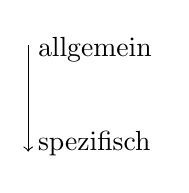
\begin{tikzpicture}
\node[right] at (0,0){spezifisch};
\node[right] at (0,1.2){allgemein};
\draw[<-] (0,-.1)--(0,1.25);
%\draw[<-] (0,.3)--(0,1);
\end{tikzpicture}

\end{minipage}

\begin{itemize}
	\item Notation verschiedener \textbf{Kontexte}:
	\begin{itemize}
		\item Silbengrenze: \$ oder: Silbenanfang: $_\sigma[$ und Silbenende: $]_\sigma$
		\item betonte Silbe: \textprimstress$\sigma$
		\item Koda: \underline{\quad}$_{\textsubscript{K}}$
		\item Morphemgrenze ($=$ Morphemanfang bzw.\ -ende): $+$
		\item Wortgrenze: \#
		\item \{ \dots\ ; \dots\ \} Liste von Kontexten, von denen nur einer gegeben sein muss
	\end{itemize}

\end{itemize}

\end{frame}


%%%%%%%%%%%%%%%%%%%%%%%%%%%%%%%%%
\subsection{Hausaufgabe}
%%%%%%%%%%%%%%%%%%%%%%%%%%%%%%%%%

\begin{frame}
\frametitle{Hausaufgabe}
\begin{itemize}
	\item[1.] Ordnen Sie die Artikulationsorte und -organe (Buchstaben) den entsprechenden Bezeichnungen (Klammern) zu.
	
\begin{minipage}{0.48\textwidth}
	\begin{figure}
		\centering
		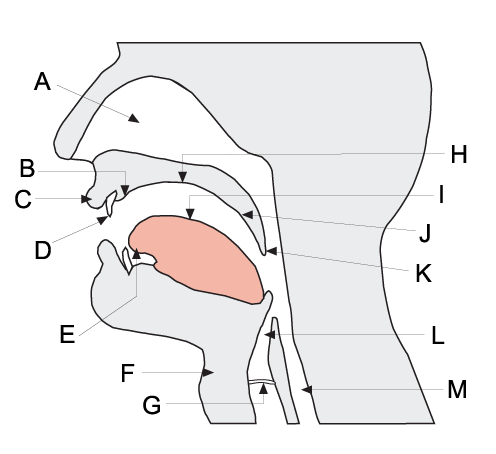
\includegraphics[scale=0.33]{material/04phonoatonomy}
	\end{figure}
\end{minipage}
\hfill
\begin{minipage}{0.4\textwidth}
	
		(~~) Stimmritze (glottal)\\
		(~~) Kehlkopf (laryngal)\\
		(~~) Zahndamm (alveolar)\\
		(~~) Nasenraum (nasal)\\
		(~~) harter Gaumen (palatal)\\
		(~~) Zähne (dental)\\
		(~~) weicher Gaumen (velar)\\
		(~~) Zungenrücken (dorsal)\\
		(~~) Halszäpfchen (uvular)\\
		(~~) Lippen (labial)\\
		(~~) Zungenspitze (apikal)
\end{minipage}

\end{itemize}
\end{frame}


%%%%%%%%%%%%%%%%%%%%%%%%%%%%%%%%
\begin{frame}{Hausaufgabe}
\begin{itemize}
	\item[2.] Welcher Laut passt jeweils nicht in die folgenden Reihen?\\
                  Begründen Sie Ihre Entscheidungen.
	
	\ea \label{ex:03aHA2}
		\ea \textipa{[b]}, \textipa{[z]}, \textipa{[a]}, \textipa{[g]}, \textipa{[v]}, \textipa{[p]}, \textipa{[u]}
		\ex \textipa{[t]}, \textipa{[s]}, \textipa{[n]}, \textipa{[\c{c}]}, \textipa{[l]}, \textipa{[d]}, \textipa{[r]}
		\ex \textipa{[f]}, \textipa{[s]}, \textipa{[x]}, \textipa{[h]}, \textipa{[r]}, \textipa{[z]}
		\ex \textipa{[N]}, \textipa{[m]}, \textipa{[k]}, \textipa{[g]}
		\ex \textipa{[m]}, \textipa{[b]}, \textipa{[N]}, \textipa{[p]}
		\z
	\z
	
	\item[3.] Geben Sie die \textbf{phonologische Repräsentation} der folgenden Wörter und \textbf{verschiedene phonetische Realisierungen} (\zB im Paradigma) an und \textbf{erläutern} Sie anschließend den \textbf{Unterschied} zwischen letzteren.
	
	\ea \label{ex:03aHA3}
		\ea Dieb
		\ex König
		\ex eng
		\z
	\z
	
\end{itemize}

\end{frame}


%%%%%%%%%%%%%%%%%%%%%%%%%%%%%%%%%
\begin{frame}{Hausaufgabe}

\begin{itemize}
	\item[4.] Bestimmen Sie, ob es sich bei den folgenden Lautkombinationen um Affrikaten handeln kann. Begründen Sie Ihre Entscheidungen.
	
	\ea \label{ex:03aHA4}
		\ea \textipa{[kl]}
		\ex \textipa{[pf]}
		\ex \textipa{[st]}
		\ex \textipa{[tr]}
		\ex \textipa{[ts]}
		\z
	\z
	
\end{itemize}

\end{frame}


%%%%%%%%%%%%%%%%%%%%%%%%%%%%%%%%%
\iftoggle{ha-loesung}{
	%%%%%%%%%%%%%%%%%%%%%%%%%%%%%%%%%%
%% HA 1 - 03a Phonologie
%%%%%%%%%%%%%%%%%%%%%%%%%%%%%%%%%%

\begin{frame}
\frametitle{Hausaufgabe -- Lösung}
\begin{itemize}
	\item[1.] Ordnen Sie die Artikulationsorte und -organe (Buchstaben) den entsprechenden Bezeichnungen (Klammern) zu.
	
	\begin{minipage}{0.48\textwidth}
		\begin{figure}
			\centering
			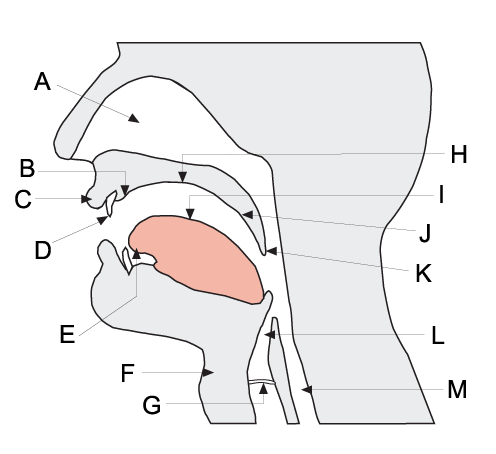
\includegraphics[scale=0.33]{material/04phonoatonomy}
		\end{figure}
	\end{minipage}
	\hfill
	\begin{minipage}{0.4\textwidth}
		
		(\visible<2->{\alertred{G}}) Stimmritze (glottal)\\
		(\visible<3->{\alertred{F}}) Kehlkopf (laryngal)\\
		(\visible<4->{\alertred{B}}) Zahndamm (alveolar)\\
		(\visible<5->{\alertred{A}}) Nasenraum (nasal)\\
		(\visible<6->{\alertred{H}}) harter Gaumen (palatal)\\
		(\visible<7->{\alertred{D}}) Zähne (dental)\\
		(\visible<8->{\alertred{J}}) weicher Gaumen (velar)\\
		(\visible<9->{\alertred{I}}) Zungenrücken (dorsal)\\
		(\visible<10->{\alertred{K}}) Halszäpfchen (uvular)\\
		(\visible<11->{\alertred{C}}) Lippen (labial)\\
		(\visible<12->{\alertred{E}}) Zungenspitze (apikal)
	\end{minipage}
	
\end{itemize}
\end{frame}


%%%%%%%%%%%%%%%%%%%%%%%%%%%%%%%%
\begin{frame}{Hausaufgabe -- Lösung}
\begin{itemize}
	\item[2.] Welcher Laut passt jeweils nicht in die folgenden Reihen?\\Begründen Sie Ihre Entscheidungen.
	
\begin{exe}
	\exr{ex:03aHA2}
\settowidth\jamwidth{XXXXXXXXXXXXXXXXXXXXXXXt}
	\begin{xlist}
		\ex \textipa{[b]}, \textipa{[z]}, \textipa{[a]}, \textipa{[g]}, \textipa{[v]}, \textipa{[p]}, \textipa{[u]} \loesung{2}{\textipa{[p]} (nicht sth., sondern stl.)}
		\ex \textipa{[t]}, \textipa{[s]}, \textipa{[n]}, \textipa{[\c{c}]}, \textipa{[l]}, \textipa{[d]}, \textipa{[r]} \loesung{3}{\textipa{[ç]} (nicht alveolar, sondern palatal)}
		\ex \textipa{[f]}, \textipa{[s]}, \textipa{[x]}, \textipa{[h]}, \textipa{[r]}, \textipa{[z]}
		\loesung{4}{\textipa{[r]} (kein Frikativ, sondern Vibrant)}
		\ex \textipa{[N]}, \textipa{[m]}, \textipa{[k]}, \textipa{[g]}
		\loesung{5}{\textipa{[k]} (nicht sth., sondern stl.)}\loesung{6}{oder: \textipa{[m]} (nicht velar, sondern labial)}
		\ex \textipa{[m]}, \textipa{[b]}, \textipa{[N]}, \textipa{[p]}
		\loesung{7}{\textipa{[N]} (nicht labial, sondern velar)} \loesung{8}{oder: \textipa{[p]} (nicht sth., sondern stl.)}
	\end{xlist}
\end{exe}
	
\end{itemize}
\end{frame}


%%%%%%%%%%%%%%%%%%%%%%%%%%%%%%%%
\begin{frame}{Hausaufgabe -- Lösung}
\begin{itemize}
	\item[3.] Geben Sie die \textbf{phonologische Repräsentation} der folgenden Wörter und \textbf{verschiedene phonetische Realisierungen} (\zB im Paradigma) an und \textbf{erläutern} Sie anschließend den \textbf{Unterschied} zwischen letzteren.
	
\begin{exe}
	\exr{ex:03aHA3}
	\settowidth\jamwidth{XXXXXXXXXXXXXXXXXXXXXXXXXXXXXXXXXXXXXXt}
	\begin{xlist}
		\ex Dieb
		\loesung{2}{\textipa{/di:b/}: \textipa{[di:p], [di:.bə]} -- Auslautverhärtung des \textipa{/b/} in der Koda}
		\ex König
		\loesung{3}{\textipa{/k\o :nıg/}: \textipa{[k\super h\o:.nıç], [k\super h\o:.nı.gə]} --} \loesung{3}{Spirantisierung des \textipa{/g/} in der Koda}
		\ex eng
		\loesung{4}{\textipa{/εng/}: \textipa{[PεN]}, (gegebenenfalls (dialektal) \textipa{[PENk]} -- g-Elision)}
	\end{xlist}
\end{exe}

\end{itemize}

\end{frame}


%%%%%%%%%%%%%%%%%%%%%%%%%%%%%%%%%
\begin{frame}{Hausaufgabe -- Lösung}

\begin{itemize}
	\item[4.] Bestimmen Sie, ob es sich bei den folgenden Lautkombinationen um Affrikaten handeln kann. Begründen Sie Ihre Entscheidungen.

\begin{exe}	
	\exr{ex:03aHA4}
\settowidth\jamwidth{XXXXXXXXXXXXXXXXXXXXXXXXXXXXXXXXXXXXXXX}
	\begin{xlist}
		\ex \textipa{[kl]} \loesung{2}{keine Affrikate (Zweitglied ist kein Frikativ)}
		\ex \textipa{[pf]} \loesung{3}{Affrikate (Verbindung aus Plosiv und homorganem Frikativ)}
		\ex \textipa{[st]} \loesung{4}{keine Affrikate (Plosiv ist Zweitglied)}
		\ex \textipa{[tr]} \loesung{5}{keine Affrikate (Zweitglied ist kein Frikativ)}
		\ex \textipa{[ts]} \loesung{6}{Affrikate (Verbindung aus Plosiv und homorganem Frikativ)}
	\end{xlist}
\end{exe}

\end{itemize}

\end{frame}



}
%%%%%%%%%%%%%%%%%%%%%%%%%%%%%%%%%



%%%%%%%%%%%%%%%%%%%%%%%%%%%%%%%%%%%%%%%%%%%%%%%%
%% Compile the master file!
%% 		Slides: Stefan Müller
%% 		Course: GK Linguistik
%%%%%%%%%%%%%%%%%%%%%%%%%%%%%%%%%%%%%%%%%%%%%%%%

%\exewidth{(35)} im übergeordneten File

% sollte zentral geladen werden. St. Mü. 04.11.2016 (in localcommands?)
%%%%%%%%%%%%%
%%% Forestset Syllables

\newbox\foreststrutbox
\setbox\foreststrutbox=\hbox to 0pt{\phantom{\forestOve{standard node}{content}}}
\def\foreststrut{\copy\foreststrutbox}
\forestset{
GP1/.style 2 args={
for n={1}{baseline},
s sep=0pt, l sep=0pt,
for descendants={
l sep=0pt, l={#1},
anchor=base,calign=first,child anchor=north,
inner xsep=1pt,inner ysep=2pt,outer sep=0pt,s sep=0pt,
},
delay={
if content={}{phantom}{for children={no edge}},
for tree={
if content={O}{tier=OR}{},
if content={R}{tier=OR}{},
if content={N}{tier=N}{},
if content={x}{
tier=x,content={$\times$},outer xsep={#2},
for tree={calign=center},
for descendants={content format={\foreststrut\forestoption{content}}},
before drawing tree={outer xsep=0pt,delay={typeset node}},
s sep=4pt
}{},
},
},
before drawing tree={where content={}{parent anchor=center,child anchor=center}{}},
},
GP1/.default={5ex}{8.0pt},
associate/.style={%
tikz+={\draw(!)--(!#1);}},
spread/.style={
before drawing tree={tikz+={\draw[dotted](!)--(!#1);}}},
govern/.style={
before drawing tree={tikz+={\draw[->](!)--(!#1);}}},
p-govern/.style={
before drawing tree={tikz+={\draw[->](.north) to[out=150,in=30] (!#1.north);}}},
no p-govern/.style={
before drawing tree={tikz+={\draw[->,loosely dashed](.north) to[out=150,in=30] (!#1.north);}}},
encircle/.style={before drawing tree={circle,draw,inner sep=0pt}},
fen/.style={pin={[font=\footnotesize,inner sep=1pt,pin edge=<-]10:\textsc{Fen}}},
el/.style={content=\textsc{\textbf{##1}}},
head/.style={content=\textsc{\textbf{\underline{##1}}}},
llap/.style={
tikz+={%
\edef\forest@temp{\noexpand\node[\option{node options},
anchor=base east,at=(.base east)]}%
\forest@temp{#1\phantom{\option{environment}}};
}
},
rlap/.style={
tikz+={%
\edef\forest@temp{\noexpand\node[\option{node options},
anchor=base west,at=(.base west)]}%
\forest@temp{\phantom{\option{environment}}#1};
}
},
}
%%%%%%%%%%%%%


%%%%%%%%%%%%%%%%%%%%%%%%%%%%%%%%%%%%%%%%%%%%%%%%%%%%
%%%             Metadata                         
%%%%%%%%%%%%%%%%%%%%%%%%%%%%%%%%%%%%%%%%%%%%%%%%%%%% 

\title{Grundkurs Linguistik}

\subtitle{Phonologie II: Silbe}

\author[St. Mü.]{
	{\small Stefan Müller}
	\\
	{\footnotesize \url{https://hpsg.hu-berlin.de/~stefan/}}
	%	\\
	%	\href{mailto:mapriema@hu-berlin.de}{mapriema@hu-berlin.de}}
}

\institute{Institut für deutsche Sprache und Linguistik}


% bitte lassen, sonst kann man nicht sehen, von wann die PDF-Datei ist.
%\date{ }

%\publishers{\textbf{6. linguistischer Methodenworkshop \\ Humboldt-Universität zu Berlin}}

%\hyphenation{nobreak}


%%%%%%%%%%%%%%%%%%%%%%%%%%%%%%%%%%%%%%%%%%%%%%%%%%%%
%%%             Preamble's End                  
%%%%%%%%%%%%%%%%%%%%%%%%%%%%%%%%%%%%%%%%%%%%%%%%%%%%   


%%%%%%%%%%%%%%%%%%%%%%%%%   
\huberlintitlepage[22pt]
\iftoggle{toc}{
\frame{
%\begin{multicols}{2}
	\frametitle{Inhaltsverzeichnis}
	\tableofcontents
	%[pausesections]
%\end{multicols}
}
}

%%%%%%%%%%%%%%%%%%%%%%%%%%%%%%%%%%
%%%%%%%%%%%%%%%%%%%%%%%%%%%%%%%%%%
%%%%%LITERATURE:

%% Allgemein
\nocite{Glueck&Roedel16a}
\nocite{Schierholz&Co18}
\nocite{Luedeling2009a}
\nocite{Meibauer&Co07a} 
\nocite{Repp&Co15a} 

%%% Sprache & Sprachwissenschaft
%\nocite{Fries16c} %Adäquatheit
%\nocite{Fries16a} %Grammatikalität
%\nocite{Fries&MyP16c} %GG
%\nocite{Fries&MyP16b} %Akzeptabilität
%\nocite{Fries&MyP16d} %Kompetenz vs. Performanz

%% Phonetik & Phonologie
\nocite{Altmann&Co07a}
\nocite{DudenAussprache00a}
\nocite{Hall00a} 
\nocite{Kohler99a}
\nocite{Krech&Co09a}
\nocite{Pompino95a}
\nocite{Ramers08a}
\nocite{Ramers&Vater92a}
\nocite{Rues&Co07a}
\nocite{WieseR96a}
\nocite{WieseR11a}


%%%%%%%%%%%%%%%%%%%%%%%%%%%%%%%%%%
%%%%%%%%%%%%%%%%%%%%%%%%%%%%%%%%%%
\section{Phonologie II: Silbe}
%%%%%%%%%%%%%%%%%%%%%%%%%%%%%%%%%%

%@EE: Checken: Struktur -- Reihenfolge der Folien
%@EE: Checken: Inhaltsverzeichnisse usw.
%@EE: Checken: wenn 3b und 3c stehen, kann der auskommentierte Text am Ende von 3b gelöscht werden

%%%%%%%%%%%%%%%%%%%%%%%%%%%%%%%%%%

\begin{frame}
\frametitle{Begleitlektüre}

\begin{itemize}
	\item \textbf{obligatorisch:}
	\begin{itemize}
		\item[] AM S.~18--23
	\end{itemize}
	\item \textbf{optional:}
	\begin{itemize}
		\item[] \citet{Hall00a}: Kapitel~8 (S.~205--230)
	\end{itemize}
\end{itemize}

\end{frame}


%%%%%%%%%%%%%%%%%%%%%%%%%%%%%%%%%%%%
%%%%%%%%%%%%%%%%%%%%%%%%%%%%%%%%%
\subsection{Einführung}

%% MyP: Contents
\iftoggle{sectoc}{
	\frame{
		%\begin{multicols}{2}
		\frametitle{~}
		\tableofcontents[currentsubsection, subsubsectionstyle=hide]
		%\end{multicols}
	}
}

%% StM: Contents
\iftoggle{gliederung}{
	
	\outline{
		\begin{itemize}
			
			\item \blaubf{Einführung}
			\item Silbenbestimmung
			\item Silbenstruktur
			%% Onset
			%% Nukleus
			%% Koda
			\item Phonotaktik
			%% Sonoritätshierarchie
			%% Weitere phonotaktische Beschränkungen
			\item Hausaufgabe
			
		\end{itemize}
	}
}
%%%%%%%%%%%%%%%%%%%%%%%%%%%%%%%%%%%
\begin{frame}
\frametitle{Einführung: Notation}


\begin{itemize}
	\item graphematische Notation in spitzen Klammern: 
	
	  \ea
          \ab{nordwind}, \ab{Nordwind}
          \z
% zwei Varianten, eine phonographisches Prinzip, eine mit syntaktischer Info = Großschreibung
          
	\item[]	
	\item phonetische Notation in eckigen Klammern:
	
	  \ea
          \textipa{[nO5t.vInt]}
	  \z
          
	\item[]
	\item phonologische Notation in Schrägstrichen:
	
	  \ea
          \textipa{/nO\textscr d.vInd/}
	  \z
\end{itemize}

\end{frame}



%%%%%%%%%%%%%%%%%%%%%%%%%%%%%%%%%%%
\begin{frame}
\frametitle{Silben}

Warum nimmt man Silben an?

\begin{itemize}
	\item Die Auslautverhärtung mit Bezug auf das Wort (vorläufig):
	
	\ea {}[$-$son] $\rightarrow$ [$-$sth] /\_\_ \#
             
	{\small (ein nicht-sonoranter Laut -- d.\,h.\ Obstruent -- wird am Wortende nicht-stimmhaft)}
	\z
     
	\item Transkribieren Sie: (\emph{sie}) \emph{siegte}

% Auslautverhärtung auch bei Silben
\pause	

	\ea
	\textipa{[zi:k . t@]} (\gqq{.} steht für Silbengrenze)
	\z

%\pause
%
%	\eal 
%	\ex \textipa{[St\textscr e:p.za:m]} \vs \textipa{[St\textscr e:.b5]}
%	\ex \textipa{[bYnt.nIs]} \vs \textipa{[bUn.d@s]}
%	\ex \textipa{[bi:k.za:m]} \vs \textipa{[bi:.g@n]}
%	\ex \textipa{[le:s.b5]} \vs \textipa{[le:.z@n]}
%    \zl
%        
%	\item Auslautverhärtung mit Bezug auf die \textbf{Silbe}:
%	  \ea
%             {}[$-$son] $\rightarrow$ [$-$sth] /\_\_ $]_{\sigma}$
%	  \z	
\end{itemize}

\end{frame}


%%%%%%%%%%%%%%%%%%%%%%%%%%%%%%%%%%%
\begin{frame}
\frametitle{Silben}

\begin{itemize}
	\item Vergleichen Sie:

\ea 

\begin{tabular}[t]{lllclll}
\only<1->{a. \ab{stre\alertred{b}sam} & \vs & \ab{Stre\alertred{b}er} &} \only<2->{~ & \textipa{[St\textscr e:\alertred{p}.za:m]} & \vs & \textipa{[St\textscr e:.\alertred{b}5]}}\\

\only<1->{b. \ab{Bün\alertred{d}nis} & \vs & \ab{Bun\alertred{d}es} &} \only<3->{~ & \textipa{[bYn\alertred{t}.nIs]} & \vs & \textipa{[bUn.\alertred{d}@s]}}\\

\only<1->{c. \ab{bie\alertred{g}sam} & \vs & \ab{bie\alertred{g}en} &} \only<4->{& \textipa{[bi:\alertred{k}.za:m]} & \vs &  \textipa{[bi:.\alertred{g}@n]}} \\

\only<1->{d. \ab{le\alertred{s}bar} & \vs & \ab{le\alertred{s}en} &} \only<5->{& \textipa{[le:\alertred{s}.b5]} & \vs &  \textipa{[le:.\alertred{z}@n]}} \\

\end{tabular}

\z 

%\begin{columns}
%\begin{column}[t]{.5\linewidth}
%\eal 
%	\ex \ab{stre\alertred{b}sam} \vs \ab{Stre\alertred{b}er}
%	\ex \ab{Bün\alertred{d}nis} \vs \ab{Bun\alertred{d}es} 
%	\ex \ab{bie\alertred{g}sam} \vs \ab{bie\alertred{g}en}
%	\ex \ab{le\alertred{s}bar} \vs \ab{le\alertred{s}en}
%\zl	
%\end{column}
%
%%\pause 
%
%\begin{column}[t]{\linewidth}
%\begin{itemize}
%%\eal 
%%\ex 
%	\item[] \textipa{[St\textscr e:\alertred{p}.za:m]} \vs \textipa{[St\textscr e:.\alertred{b}5]}
%%\ex 
%	\item[] \textipa{[bYn\alertred{t}.nIs]} \vs \textipa{[bUn.\alertred{d}@s]}
%%\ex 
%	\item[] \textipa{[bi:\alertred{k}.za:m]} \vs \textipa{[bi:.\alertred{g}@n]}
%%\ex 
%	\item[] \textipa{[le:\alertred{s}.b5]} \vs \textipa{[le:.\alertred{z}@n]}
%%\zl
%\end{itemize}
%\end{column}
%
%\end{columns}	
\end{itemize}


\begin{itemize}
	\item<6-> Auslautverhärtung mit Bezug auf die \textbf{Silbe}:
	\ea
	{}[$-$son] $\rightarrow$ [$-$sth] /\_\_ $]_{\sigma}$
	\z	
\end{itemize}

\end{frame}


%%%%%%%%%%%%%%%%%%%%%%%%%%%%%%%%%%%
\begin{frame}
\frametitle{Silben}

Warum nimmt man Silben an?

Silbe als \textbf{Domäne} \ldots

\begin{itemize}	
	\item \ldots\ verschiedener \textbf{phonologischer Prozesse}\\
               (\zB Auslautverhärtung, Knacklauteinsetzung, Aspiration, \ldots )
	
	\item[] 
	
	\item \ldots\ von Regularitäten bzgl. der \textbf{Abfolge} von Lauten
	
	\item[]
	
	\item \ldots\ der \textbf{Wortbetonung}, d.\,h. wichtige so genannte prosodische Einheiten (Prosodie $=$ Betonung mit Bezug auf Einheiten über dem Segment)
\end{itemize}

\end{frame}



%%%%%%%%%%%%%%%%%%%%%%%%%%%%%%%%%%%
%
%\begin{frame}
%\frametitle{Prosodische Konstituenten}
%
%
%	\begin{multicols}{2}
%	\begin{itemize*}
%		\item UP = Äußerungsphrase
%		\item IP = Intonationsphrase
%		\item $\phi$ = phonol. Phrase
%\columnbreak
%		\item $\omega$ = phonol. Wort
%		\item F = phonol. Fuß
%		\item \alertred{$\sigma$ = Silbe}
%	\end{itemize*}
%	\end{multicols}
%
%\begin{figure} %%rote Box einfügen
%	\centering
%	\scalebox{.68}{
%	\begin{forest} MyP edges,
%	[IP
%	[$\Phi$
%	[$\omega$[F[\alertred{$\sigma$}[Frau]]]]
%	[$\omega$[F[\alertred{$\sigma$}[Müll, name=mueller]][\alertred{$\sigma$}, name=sigma[er]]]]]
%	[$\Phi$
%	[$\omega$[F[\alertred{$\sigma$}[kauft]]]]
%	[$\omega$[F[\alertred{$\sigma$}[Steck]]]
%			 [F[\alertred{$\sigma$}[rü]]
%			   [\alertred{$\sigma$}[ben]]]]]
%	[$\Phi$
%	[$\omega$[F[\alertred{$\sigma$}[auf]]]
%			 [F[\alertred{$\sigma$}[dem]]]]
%	[$\omega$[F[\alertred{$\sigma$}[Woch, name=woch]]
%			   [\alertred{$\sigma$}, name=sigmab[en]]]
%			 [F[\alertred{$\sigma$}[markt]]]]]
%	]
%	{
%		\draw[black] (mueller.north)--(sigma.south);
%		\draw[black] (woch.north)--(sigmab.south);
%	}
%	\end{forest}
%}
%	\caption{nach C. Féry}
%	\label{Zeichen1}
%\end{figure}
%
%% Doppeltverwendung bei Silbengelenken Mül ler
%
%% betonte Silben bilden Fuß einschließlich allen folgenden unbetonten Silben
%
%%\begin{figure}[b]
%%	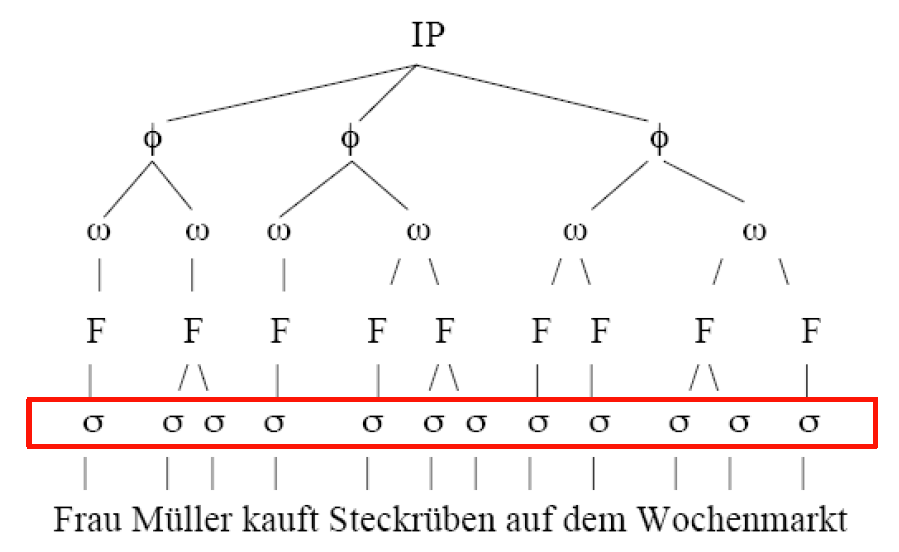
\includegraphics[scale=0.3]{material/03bHierarchieIntonationsphrase}
%%	\caption{Hierarchie in der Intonationsphrase (Darstellung von C. Féry)}
%%	\label{Zeichen1}
%%\end{figure}
%
%\end{frame}

%%%%%%%%%%%%%%%%%%%%%%%%%%%%%%%%%%%
\begin{frame}
\frametitle{Prosodische Konstituenten}

	\begin{multicols}{2}
	\begin{itemize*}
		\item UP = Äußerungsphrase
		\item IP = Intonationsphrase
		\item $\varphi$ = phonol. Phrase
\columnbreak
		\item $\omega$ = phonol. Wort
		\item F = phonol. Fuß
		\item \alertred{$\sigma$ = Silbe}
	\end{itemize*}
	\end{multicols}


	\begin{figure}
	\centering
	\scalebox{.68}{
		\begin{forest} MyP edges,
		[UP, name=up
		[IP, name=IP
		[$\varphi$[$\omega$[F[$\sigma$][$\sigma$]][F[$\sigma$][$\sigma$]]]]
		[$\varphi$, name=Phi[$\omega$[F[$\sigma$][$\sigma$]]][$\omega$, name=omega[F, name=F[$\sigma$][$\sigma$, name=sigma]]]]
		]]
		{\draw[black] (up.east)--(3,0);
			\draw[black] (IP.east)--(3,-1);
			\draw[black] (Phi.east)--(3,-2);
			\draw[black] (omega.east)--(3,-3);
			\draw[black] (F.east)--(3,-4);
			\draw[black] (sigma.east)--(3,-5.3);
			\node[right] at (3,0) {(Mandarinen oder Äpfel)\textsubscript{UP}};
			\node[right] at (3,-1) {(Mandarinen oder Äpfel)\textsubscript{IP}};
			\node[right] at (3,-2) {(Mandarinen)\textsubscript{$\varphi$} (oder Äpfel)\textsubscript{$\varphi$}};
			\node[right] at (3,-3) {(Mandarinen)\textsubscript{$\omega$} (oder)\textsubscript{$\omega$} (Äpfel)\textsubscript{$\omega$}};
			\node[right] at (3,-4) {(Manda)\textsubscript{F} (rinen)\textsubscript{F} (oder)\textsubscript{F} (Äpfel)\textsubscript{F}};
			\node[right] at (3,-5.3) {(Man)\textsubscript{$\sigma$} (da)\textsubscript{$\sigma$} (ri)\textsubscript{$\sigma$} (nen)\textsubscript{$\sigma$} (o)\textsubscript{$\sigma$} (der)\textsubscript{$\sigma$} (Äp)\textsubscript{$\sigma$} (fel)\textsubscript{$\sigma$}};
	}
		\end{forest}
	}
		\caption{\cite{Fuhrhop&Co13a}}
	\end{figure}

%\begin{figure}[b]
%	\centering
%	
%	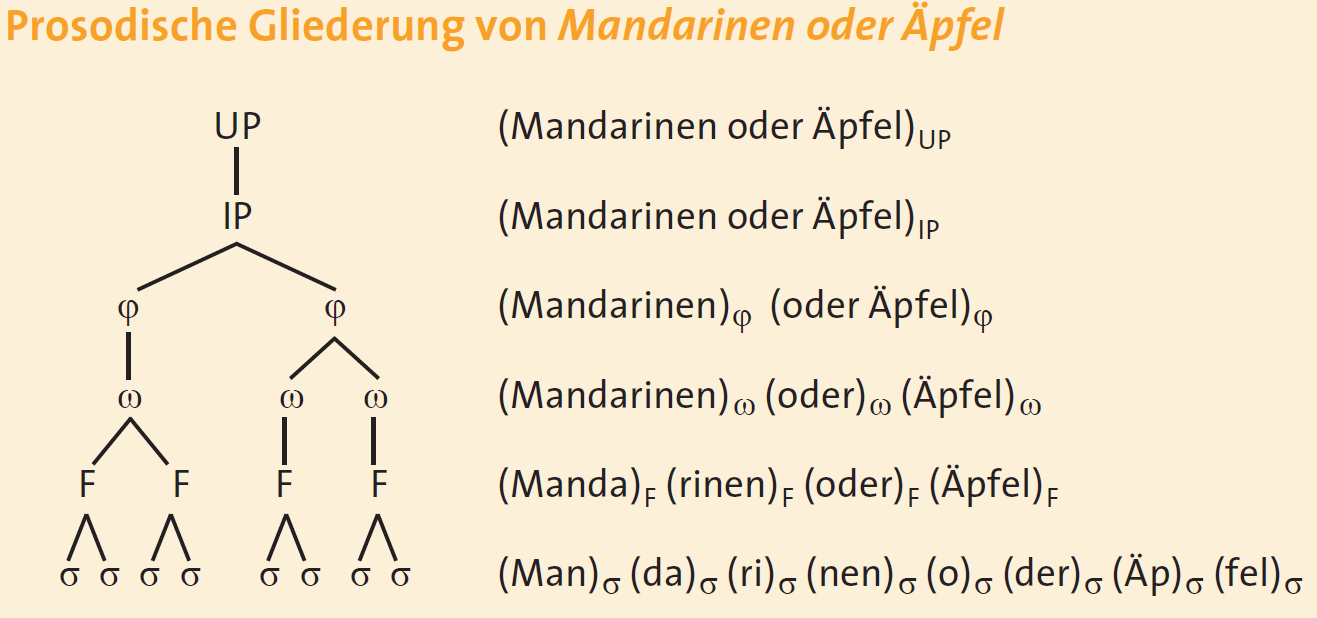
\includegraphics[scale=0.26]{material/03bHierarchieUP}
%	\caption{Hierarchie in der Äußerungsphrase \citep[8]{Fuhrhop&Co13a}}
%	%\label{Zeichen1}
%\end{figure}

\end{frame}


%%%%%%%%%%%%%%%%%%%%%%%%%%%%%%%%%%
%%%%%%%%%%%%%%%%%%%%%%%%%%%%%%%%%%
\subsection{Silbenbestimmung}

%% MyP: Contents
\iftoggle{sectoc}{
	\frame{
		%\begin{multicols}{2}
		\frametitle{~}
		\tableofcontents[currentsubsection, subsubsectionstyle=hide]
		%\end{multicols}
	}
}

%% StM: Contents
\iftoggle{gliederung}{
	
	\outline{
		\begin{itemize}
			
			\item Einführung
			\item \blaubf{Silbenbestimmung}
			\item Silbenstruktur
			%% Onset
			%% Nukleus
			%% Koda
			\item Phonotaktik
			%% Sonoritätshierarchie
			%% Weitere phonotaktische Beschränkungen
			\item Hausaufgabe
			
		\end{itemize}
	}
}
%%%%%%%%%%%%%%%%%%%%%%%%%%%%%%%%%%

\begin{frame}
\frametitle{Silbenbestimmung}

\begin{itemize}
	\item<1-> Wie viele Silben hat das folgende Wort?
	
	\ea Silbenbestimmung
	\z
	
	\item<2-> Woher wissen Sie das?
	
	\begin{itemize}
		\item[]<2-> \gqq{Jeder kompetente Sprachteilhaber verfügt über die \textbf{Fähigkeit},\\
 Silben identifizieren zu können.}  \citep[133]{Staffeldt10a}

		\vspace{.25cm}

		\item[]<2-> \gqq{Silbe: Phonetisch-phonologische \textbf{Grundeinheit} des Wortes
                  bzw.\ der Rede, die zwar \textbf{intuitiv} nachweisbar ist, wissenschaftlich aber \textbf{nicht einheitlich definiert} wird.} \citep[600]{Bussmann02a}
		
	\end{itemize}
 
	\item<3-> Silben können \textbf{betont} werden (tragen Akzent)
	
	\item<4-> \textbf{Silbenspiele} (\zB \only<5->{Sil\alertred{pi}-ben\alertred{pe}-spie\alertred{pi}-le\alertred{pe},} \only<5->{Si\alertred{hi}l-be\alertred{he}n-spie\alertred{hi}-le\alertred{he})}
% Geheimsprache, nach Silben wird immer pi, pa, pe oder so eingesetzt
	
	\item<6-> \textbf{Intuitiv} erkennbare Einheit: 
	
	Kinder können in einem sehr frühen Alter intuitiv Silben klatschen.

\end{itemize}

\end{frame}



%%%%%%%%%%%%%%%%%%%%%%%%%%%%%%%%%%
%%%%%%%%%%%%%%%%%%%%%%%%%%%%%%%%%%
\subsection{Silbenstruktur}

%% MyP: Contents
\iftoggle{sectoc}{
	\frame{
		%\begin{multicols}{2}
		\frametitle{~}
		\tableofcontents[currentsubsection, subsubsectionstyle=hide]
		%\end{multicols}
	}
}

%% StM: Contents
\iftoggle{gliederung}{
	
	\outline{
		\begin{itemize}
			
			\item Einführung
			\item Silbenbestimmung
			\item \blaubf{Silbenstruktur}
			%% Onset
			%% Nukleus
			%% Koda
			\item Phonotaktik
			%% Sonoritätshierarchie
			%% Weitere phonotaktische Beschränkungen
			\item Hausaufgabe
			
		\end{itemize}
	}
}
%%%%%%%%%%%%%%%%%%%%%%%%%%%%%%%%%%
\begin{frame}
\frametitle{Silbenstruktur}

\begin{itemize}
	\item Welche Silben (des Deutschen) sind mit den folgenden Segmenten bildbar?

\ea \textipa{[p]}, \textipa{[a]}, \textipa{[l]}, \textipa{[t]}
\z

\pause	

\begin{multicols}{2}
\ea \textbf{bildbar:}\\
	\textipa{[palt]},\\
	\textipa{[alpt]}, \\
	\textipa{[lapt]}, \\
	\textipa{[talp]}, \\
	\textipa{[plat]}
\z 

\columnbreak

\pause

	\ea \textbf{nicht bildbar:}\\
	*\textipa{[ltap]}, \\
	*\textipa{[lpat]},\\
	*\textipa{[ptla]}, \\
	*\textipa{[tpal]}, 	\ldots 
\z
\end{multicols}

\pause

\item Warum?

\end{itemize}

\end{frame}



%%%%%%%%%%%%%%%%%%%%%%%%%%%%%%%%%%%
%\begin{frame}
%\frametitle{Silbenstruktur}
%
%Die Silbe ist \textbf{intern strukturiert} und besteht aus den folgenden Teilen:
%
%\begin{minipage}{.60\textwidth}
%
%\begin{itemize}
%	\item[]
%	\item Silbenanlaut/Silbenanfangsrand/\alert{Onset},
%	\begin{itemize}
%		\item 0 bis $n$ Konsonanten, wobei in fast allen Sprachen $n < 5$
%	\end{itemize}
%	
%	\item[]
%	\item Silbengipfel/Silbenkern/\alert{Nukleus},
%	\begin{itemize}
%		\item Vokale
%		\item manchmal (vokalische) Nasale oder Liquide
%	\end{itemize}
%	
%	\item[]
%	\item Silbenauslaut/Silbenendrand/\alert{Koda}
%	\begin{itemize}
%		\item 0 bis $n$ Konsonanten, wobei in fast allen Sprachen $n < 5$
%	\end{itemize}
%
%	\item[]
%	\item Nukleus und Koda bilden den \alert{Reim}
%	
%\end{itemize}
%
%
%\end{minipage}
%\begin{minipage}{.39\textwidth}
%
%%%%%%%%%%%%%%
%%% Forestset Syllables

\newbox\foreststrutbox
\setbox\foreststrutbox=\hbox to 0pt{\phantom{\forestOve{standard node}{content}}}
\def\foreststrut{\copy\foreststrutbox}
\forestset{
GP1/.style 2 args={
for n={1}{baseline},
s sep=0pt, l sep=0pt,
for descendants={
l sep=0pt, l={#1},
anchor=base,calign=first,child anchor=north,
inner xsep=1pt,inner ysep=2pt,outer sep=0pt,s sep=0pt,
},
delay={
if content={}{phantom}{for children={no edge}},
for tree={
if content={O}{tier=OR}{},
if content={R}{tier=OR}{},
if content={N}{tier=N}{},
if content={x}{
tier=x,content={$\times$},outer xsep={#2},
for tree={calign=center},
for descendants={content format={\foreststrut\forestoption{content}}},
before drawing tree={outer xsep=0pt,delay={typeset node}},
s sep=4pt
}{},
},
},
before drawing tree={where content={}{parent anchor=center,child anchor=center}{}},
},
GP1/.default={5ex}{8.0pt},
associate/.style={%
tikz+={\draw(!)--(!#1);}},
spread/.style={
before drawing tree={tikz+={\draw[dotted](!)--(!#1);}}},
govern/.style={
before drawing tree={tikz+={\draw[->](!)--(!#1);}}},
p-govern/.style={
before drawing tree={tikz+={\draw[->](.north) to[out=150,in=30] (!#1.north);}}},
no p-govern/.style={
before drawing tree={tikz+={\draw[->,loosely dashed](.north) to[out=150,in=30] (!#1.north);}}},
encircle/.style={before drawing tree={circle,draw,inner sep=0pt}},
fen/.style={pin={[font=\footnotesize,inner sep=1pt,pin edge=<-]10:\textsc{Fen}}},
el/.style={content=\textsc{\textbf{##1}}},
head/.style={content=\textsc{\textbf{\underline{##1}}}},
llap/.style={
tikz+={%
\edef\forest@temp{\noexpand\node[\option{node options},
anchor=base east,at=(.base east)]}%
\forest@temp{#1\phantom{\option{environment}}};
}
},
rlap/.style={
tikz+={%
\edef\forest@temp{\noexpand\node[\option{node options},
anchor=base west,at=(.base west)]}%
\forest@temp{\phantom{\option{environment}}#1};
}
},
}
%%%%%%%%%%%%%

%\begin{figure}
%\centering
%\begin{forest} MyP edges, GP1 [
%  [$\sigma$
%    [O	[ [C$^{n}$]]
%    ]
%    [R	[N
%    		[V$^{n}$]
%    	]
%    	[K
%    		[C$^{n}$]
%    	]
%    ]
%  ]
%]
%\end{forest}
%\caption{Silbenstruktur}
%\end{figure}
%
%\end{minipage}
%
%\end{frame}



%%%%%%%%%%%%%%%%%%%%%%%%%%%%%%%%%%

\begin{frame}
\frametitle{Silbenstruktur: komplexe Silbe}

Die Silbe ist \textbf{intern strukturiert} und besteht aus den folgenden Teilen:

\begin{minipage}{.59\textwidth}

\begin{itemize}
	\item[]
	\item \alertred{Onset} 
	
	\item \alertred{Reim} 
	
	\item \alertred{Nukleus}
	
	\item \alertred{Koda}
	\item[] 
	\item C $:=$ konsonantisch, d.\,h. nicht-silbisch ($\neq$Konsonant)
	
	\item V $:=$ vokalisch, d.\,h. silbisch ($\neq$Vokal)
	
\end{itemize}


\end{minipage}
\begin{minipage}{.40\textwidth}

%%%%%%%%%%%%%%
%%% Forestset Syllables

\newbox\foreststrutbox
\setbox\foreststrutbox=\hbox to 0pt{\phantom{\forestOve{standard node}{content}}}
\def\foreststrut{\copy\foreststrutbox}
\forestset{
GP1/.style 2 args={
for n={1}{baseline},
s sep=0pt, l sep=0pt,
for descendants={
l sep=0pt, l={#1},
anchor=base,calign=first,child anchor=north,
inner xsep=1pt,inner ysep=2pt,outer sep=0pt,s sep=0pt,
},
delay={
if content={}{phantom}{for children={no edge}},
for tree={
if content={O}{tier=OR}{},
if content={R}{tier=OR}{},
if content={N}{tier=N}{},
if content={x}{
tier=x,content={$\times$},outer xsep={#2},
for tree={calign=center},
for descendants={content format={\foreststrut\forestoption{content}}},
before drawing tree={outer xsep=0pt,delay={typeset node}},
s sep=4pt
}{},
},
},
before drawing tree={where content={}{parent anchor=center,child anchor=center}{}},
},
GP1/.default={5ex}{8.0pt},
associate/.style={%
tikz+={\draw(!)--(!#1);}},
spread/.style={
before drawing tree={tikz+={\draw[dotted](!)--(!#1);}}},
govern/.style={
before drawing tree={tikz+={\draw[->](!)--(!#1);}}},
p-govern/.style={
before drawing tree={tikz+={\draw[->](.north) to[out=150,in=30] (!#1.north);}}},
no p-govern/.style={
before drawing tree={tikz+={\draw[->,loosely dashed](.north) to[out=150,in=30] (!#1.north);}}},
encircle/.style={before drawing tree={circle,draw,inner sep=0pt}},
fen/.style={pin={[font=\footnotesize,inner sep=1pt,pin edge=<-]10:\textsc{Fen}}},
el/.style={content=\textsc{\textbf{##1}}},
head/.style={content=\textsc{\textbf{\underline{##1}}}},
llap/.style={
tikz+={%
\edef\forest@temp{\noexpand\node[\option{node options},
anchor=base east,at=(.base east)]}%
\forest@temp{#1\phantom{\option{environment}}};
}
},
rlap/.style={
tikz+={%
\edef\forest@temp{\noexpand\node[\option{node options},
anchor=base west,at=(.base west)]}%
\forest@temp{\phantom{\option{environment}}#1};
}
},
}
%%%%%%%%%%%%%


\begin{figure}
\centering
\begin{forest} MyP edges, GP1 [
  [$\sigma$
    [O
    	[[C[\textipa{S}]]]
    	[[C[\textipa{t}]]]
    	[[C[\textipa{\textscr}]]]
    ]
    [R
    	[N
    		[V[\textipa{U}]]
    	]
    	[K
    		[C[\textipa{m}]]
    		[C[\textipa{\t{pf}}]]
    		[C[\textipa{s}]]
    		[C[\textipa{t}]]
    	]
    ]
  ]
]
\end{forest}
%\caption{Komplexe Silbe}
\end{figure}
% wahrscheinlich komplexeste Koda, die es gibt.
\end{minipage}

\end{frame}


%%%%%%%%%%%%%%%%%%%%%%%%%%%%%%%%%%
\begin{frame}
\frametitle{Silbenstruktur: minimale Silbe}

Die Silbe ist \textbf{intern strukturiert} und besteht aus den folgenden Teilen:

\begin{minipage}{.60\textwidth}

\begin{itemize}
	\item[]
	\item \alertred{Onset}
	
	\item \alertred{Reim}
	
	\item \alertred{Nukleus}
	
	\item \alertred{Koda}
	\item[] 
	\item \textbf{Minimale Silbe} besteht nur aus einem V im  Nukleus
	  \ea
          \ab{gehe} \ras \textipa{[ge:.\alertred{@}]}
          \z
	
\end{itemize}


\end{minipage}
\begin{minipage}{.39\textwidth}

%%%%%%%%%%%%%%
%%% Forestset Syllables

\newbox\foreststrutbox
\setbox\foreststrutbox=\hbox to 0pt{\phantom{\forestOve{standard node}{content}}}
\def\foreststrut{\copy\foreststrutbox}
\forestset{
GP1/.style 2 args={
for n={1}{baseline},
s sep=0pt, l sep=0pt,
for descendants={
l sep=0pt, l={#1},
anchor=base,calign=first,child anchor=north,
inner xsep=1pt,inner ysep=2pt,outer sep=0pt,s sep=0pt,
},
delay={
if content={}{phantom}{for children={no edge}},
for tree={
if content={O}{tier=OR}{},
if content={R}{tier=OR}{},
if content={N}{tier=N}{},
if content={x}{
tier=x,content={$\times$},outer xsep={#2},
for tree={calign=center},
for descendants={content format={\foreststrut\forestoption{content}}},
before drawing tree={outer xsep=0pt,delay={typeset node}},
s sep=4pt
}{},
},
},
before drawing tree={where content={}{parent anchor=center,child anchor=center}{}},
},
GP1/.default={5ex}{8.0pt},
associate/.style={%
tikz+={\draw(!)--(!#1);}},
spread/.style={
before drawing tree={tikz+={\draw[dotted](!)--(!#1);}}},
govern/.style={
before drawing tree={tikz+={\draw[->](!)--(!#1);}}},
p-govern/.style={
before drawing tree={tikz+={\draw[->](.north) to[out=150,in=30] (!#1.north);}}},
no p-govern/.style={
before drawing tree={tikz+={\draw[->,loosely dashed](.north) to[out=150,in=30] (!#1.north);}}},
encircle/.style={before drawing tree={circle,draw,inner sep=0pt}},
fen/.style={pin={[font=\footnotesize,inner sep=1pt,pin edge=<-]10:\textsc{Fen}}},
el/.style={content=\textsc{\textbf{##1}}},
head/.style={content=\textsc{\textbf{\underline{##1}}}},
llap/.style={
tikz+={%
\edef\forest@temp{\noexpand\node[\option{node options},
anchor=base east,at=(.base east)]}%
\forest@temp{#1\phantom{\option{environment}}};
}
},
rlap/.style={
tikz+={%
\edef\forest@temp{\noexpand\node[\option{node options},
anchor=base west,at=(.base west)]}%
\forest@temp{\phantom{\option{environment}}#1};
}
},
}
%%%%%%%%%%%%%


\begin{figure}
\centering
\begin{forest} MyP edges, GP1 [
  [$\sigma$
    [O
    ]
    [R
    	[N
    		[V[\textipa{@}]]
    	]
    	[K
    	]
    ]
  ]
]
\end{forest}
%\caption{Minimale Silbe}
\end{figure}


\end{minipage}

\end{frame}


%%%%%%%%%%%%%%%%%%%%%%%%%%%%%%%%%%
\begin{frame}
\frametitle{Offene/geschlossene/nackte/bedeckte Silben}

\begin{itemize}
	\item Silbenanlaut/Silbenanfangsrand/\alertred{Onset},
	\item Silbengipfel/Silbenkern/\alertred{Nukleus},
	\item Silbenauslaut/Silbenendrand/\alertred{Koda}
	
\end{itemize}

\begin{table}
\centering
\begin{tabular}{lllll}
\textsc{Onset} & \textsc{Nukleus} & \textsc{Koda} & \textsc{Term} & \textsc{Merkmal} \\
\hline
\textipa{z} & \textipa{e:} & & offene Silbe & Koda: leer\\
\hline
\textipa{t} & \textipa{a:} & \textipa{l} & geschlossene Silbe & Koda: besetzt\\
\hline
 & \textipa{@} & \textipa{n} & nackte Silbe & Onset: leer\\
\hline
\textipa{z} & \textipa{e:} & & bedeckte Silbe & Onset: besetzt\\
\end{tabular}
\end{table}

\end{frame}



%%%%%%%%%%%%%%%%%%%%%%%%%%%%%%%%%
%%%%%%%%%%%%%%%%%%%%%%%%%%%%%%%%%
\subsubsection{Onset}
%\frame{
%\begin{multicols}{2}
%\frametitle{~}
%	\tableofcontents[currentsection]
%\end{multicols}
%}
%%%%%%%%%%%%%%%%%%%%%%%%%%%%%%%%%

\begin{frame}
\frametitle{Onset}

Im Deutschen sind
	\begin{itemize}
		\item \textbf{3 Cs} beschränkt: \textipa{/S/} oder \textipa{/s/} $+$ stl. Plosiv $+$ Liquid (\zB \textbf{Spl}itter, \textbf{Skl}ave),
		\item \textbf{2 Cs} oft (\zB \textipa{/bl/}, \textipa{/kn/} \dots\ ) und
		\item \textbf{1 C} immer (bis auf \textipa{[N]}) möglich.
	\end{itemize}
	
	
Maximale Onset-Belegung in verschiedenen Sprachen:


\eal
\ex Deutsch \textipa{[\alertred{St\textscr}aIt]} \gq{Streit}
\ex Tschechisch \textipa{[\alertred{fspl}a.nout]} \gq{aufflammen}
\ex Hawaianisch \textipa{[a.\alertred{l}o.\alertred{h}a]} \gq{Liebe}
\zl

\end{frame}

%%%%%%%%%%%%%%%%%%%%%%%%%%%%%%%%%%
\begin{frame}
\frametitle{Onset: Silbenanlautgesetz}

\begin{itemize}
	\item Bei Betrachtung aller (bekannten) Sprachen kann man die folgende Gesetzmäßigkeit feststellen \citep[cf.][212f.]{Hall00a}:
	
\medskip
	\begin{block}{Silbenanlautgesetz}
	
	\sub{$\sigma$}[CV $>$ \sub{$\sigma$}[V 
	und
	\sub{$\sigma$}[C\MyPup{$n$}V $>$ \sub{$\sigma$}[C\MyPup{$n+1$}V (wobei $n \geq 1$)
	
	$>$ $:=$ \gq{häufiger als} oder \gq{ist weniger markiert als}

% Silbe mit Konsonant und Vokal sind häfiger als solche, die nur mit Vokal beginnen
% Silbe mit n Konsonanten ist weniger markiert als Silbe mit n+1 KOnsonanten.
	
	\end{block}
\medskip
	 
	 \item Man spricht auch von der \textbf{Markiertheit} von Silben,\\
	 wenn sie Präferenzgesetzen widersprechen.

\end{itemize}

\end{frame}


%%%%%%%%%%%%%%%%%%%%%%%%%%%%%%%%%%
%%%%%%%%%%%%%%%%%%%%%%%%%%%%%%%%%%
\subsubsection{Nukleus}
%\frame{
%\begin{multicols}{2}
%\frametitle{~}
%	\tableofcontents[currentsection]
%\end{multicols}
%}
%%%%%%%%%%%%%%%%%%%%%%%%%%%%%%%%%%

\begin{frame}
\frametitle{Nukleus: Silbenkerngesetz}

\begin{itemize}

	\item In \emph{allen} Sprachen werden Nuklei durch \textbf{Vokale} (V) gebildet.
	
	\item In \emph{einigen} Sprachen können Nuklei auch durch \textbf{Liquide} und \textbf{Nasale} (C \vs V) gebildet werden.

	\item Im Deutschen werden bei schnellem Sprechen folgende Wörter mit sogenannten \textbf{silbischen Konsonanten} gesprochen
	
	\begin{multicols}{2}
          \ea
          \ab{lesen} \textipa{[le:.z\alertred{\textsyllabic{n}}]}
          \z
          
          \ea
          \ab{Wandel} \textipa{[van.d\alertred{\textsyllabic{l}}]}
          \z
	\end{multicols}

\pause 

	\item Bei Betrachtung aller (bekannten) Sprachen kann man die folgende Gesetzmäßigkeit feststellen \citep[cf.][217f.]{Hall00a}:

\end{itemize}
	
	\begin{block}{Silbenkerngesetz}
		
	Vokale $>$ Sonoranten $>$ Obstruenten\\
	Silben mit einfachem vokalischem Nukleus sind universell bevorzugt.
	\end{block}
	
\end{frame}



%%%%%%%%%%%%%%%%%%%%%%%%%%%%%%%%%%
%%%%%%%%%%%%%%%%%%%%%%%%%%%%%%%%%%
\subsubsection{Koda}
%\frame{
%\begin{multicols}{2}
%\frametitle{~}
%	\tableofcontents[currentsection]
%\end{multicols}
%}
%%%%%%%%%%%%%%%%%%%%%%%%%%%%%%%%%%

\begin{frame}
\frametitle{Koda: Silbenauslautgesetz}

In der Koda sind/ist \ldots

\begin{itemize}

	\item \ldots\ in \emph{vielen} Sprachen keine Konsonanten erlaubt (\zB Hawaiianisch),
	
	\item \ldots\ in \emph{einigen} Sprachen ein Konsonant erlaubt,
	
	\item \ldots\ in \emph{einigen (wenigen)} Sprachen mehrere Konsonanten erlaubt.
	
	\item[]
	\item Deutsch: \textipa{[hE\alertred{\textscr psts}]} (0 bis 4/5 Konsonanten)
	
	\item Reihenfolge der Konsonanten unterliegt dem  \textbf{Sonoritätsprinzip}
	
	\item Bei Betrachtung aller (bekannten) Sprachen kann man die folgende Gesetzmäßigkeit feststellen \citep[cf.][214]{Hall00a}:

\end{itemize}
	
	\begin{block}{Silbenauslautgesetz}
	
	CVC$^{n}$]$_{\sigma}$ $>$ CVC$^{n+1}$]$_{\sigma}$ (wobei $n \geq 0$)
	
	\end{block}
	
\end{frame}



%%%%%%%%%%%%%%%%%%%%%%%%%%%%%%%%%%%
%%%%%%%%%%%%%%%%%%%%%%%%%%%%%%%%%%%
\subsection{Phonotaktik}

%% MyP: Contents
\iftoggle{sectoc}{
	\frame{
		%\begin{multicols}{2}
		\frametitle{~}
		\tableofcontents[currentsubsection, subsubsectionstyle=hide]
		%\end{multicols}
	}
}

%% StM: Contents
\iftoggle{gliederung}{
	
	\outline{
		\begin{itemize}
			
			\item Einführung
			\item Silbenbestimmung
			\item Silbenstruktur
			%% Onset
			%% Nukleus
			%% Koda
			\item \blaubf{Phonotaktik}
			%% Sonoritätshierarchie
			%% Weitere phonotaktische Beschränkungen
			\item Hausaufgabe			
			
		\end{itemize}
	}
}
%%%%%%%%%%%%%%%%%%%%%%%%%%%%%%%%%%

\begin{frame}
\frametitle{Phonotaktik}

\begin{block}{Phonotaktik}

Die Phonotaktik untersucht die syntagmatischen Beziehungen zwischen Lauten innerhalb der Silbe und anderer prosodischer Einheiten \citep{Fuhrhop&Co13a}.

\end{block}

\begin{itemize}
	\item Mögliche und unmögliche Kombinationen von Segmenten bzgl.
	
	\begin{itemize}
		\item Anzahl der Laute,
		\item Art,
		\item Reihenfolge der Laute.
	\end{itemize}

\end{itemize}

\end{frame}



%%%%%%%%%%%%%%%%%%%%%%%%%%%%%%%%%%
%%%%%%%%%%%%%%%%%%%%%%%%%%%%%%%%%%
\subsubsection{Sonoritätshierarchie}
%\frame{
%\begin{multicols}{2}
%\frametitle{~}
%	\tableofcontents[currentsection]
%\end{multicols}
%}
%%%%%%%%%%%%%%%%%%%%%%%%%%%%%%%%%%

\begin{frame}
\frametitle{Sonoritätshierarchie}

\begin{itemize}
	\item Betrachten Sie die folgenden Beispiele und überlegen Sie \ldots
	
	\begin{enumerate}
		\item \ldots\ welche \textbf{phonotaktischen Beschränkungen} für den Onset in deutschen Silben gelten könnten:

                  \ea
                  \textipa{[\alertred{k\textscr}aNk]}, \textipa{[\alertred{pl}a:n]}, \textipa{[\alertred{f\textscr}E\c{c}]},
                  \textipa{[\alertred{fl}o:]}, \textipa{[\alertred{kn}i:]}, \textipa{[\alertred{gn}a:d@]}
                  \z

                  \ea
                  *\textipa{[\alertred{{\textscr}k}aNk]}, *\textipa{[\alertred{lp}a:n]}, *\textipa{[\alertred{{\textscr}f}E\c{c}]}, *\textipa{[\alertred{lf}o:]}, *\textipa{[\alertred{nk}i:]}, *\textipa{[\alertred{ng}a:d@]}
                  \z
                  
\pause
		\item \ldots\ welche \textbf{phonotaktischen Beschränkungen} für die Koda in deutschen Silben gelten könnten:

                  \ea
                  \textipa{[ka\alertred{lt}]}, \textipa{[ha\alertred{{\textscr}t}]}, \textipa{[la\alertred{nt}]}, \textipa{[k{\textscr}a\alertred{Nk}]}
                  \z

                  \ea
                  *\textipa{[ka\alertred{tl}]}, *\textipa{[ha\alertred{t\textscr}]}, *\textipa{[la\alertred{tn}]},
                  *\textipa{[k\textscr a\alertred{kN}]}
                  \z

	\end{enumerate}
	
\end{itemize}

\end{frame}



%%%%%%%%%%%%%%%%%%%%%%%%%%%%%%%%%%
\begin{frame}
\frametitle{Sonoritätshierarchie}

\begin{enumerate}
	\item phonotaktische Beschränkungen für den Onset
	
          \ea
          \textipa{[\alertred{k\textscr}aNk]}, \textipa{[\alertred{pl}a:n]}, \textipa{[\alertred{f\textscr}E\c{c}]},
          \textipa{[\alertred{fl}o:]}, \textipa{[\alertred{kn}i:]}, \textipa{[\alertred{gn}a:d@]}
          \z

          \ea
          *\textipa{[\alertred{{\textscr}k}aNk]}, *\textipa{[\alertred{lp}a:n]}, *\textipa{[\alertred{{\textscr}f}E\c{c}]}, *\textipa{[\alertred{lf}o:]}, *\textipa{[\alertred{nk}i:]}, *\textipa{[\alertred{ng}a:d@]}
          \z

	\item phonotaktische Beschränkungen für die Koda

          \ea
          \textipa{[ka\alertred{lt}]}, \textipa{[ha\alertred{5t}]}, \textipa{[la\alertred{nt}]}, \textipa{[k\textscr a\alertred{Nk}]}
          \z

          \ea
          *\textipa{[ka\alertred{tl}]}, *\textipa{[ha\alertred{t\textscr}]}, *\textipa{[la\alertred{tn}]}, *\textipa{[k\textscr
              a\alertred{kN}]}
          \z

\end{enumerate}
	

\begin{table}
\centering
\begin{tabular}{c|c|c|c|c} 
 & Sonorant & Obstruent & Vokal & Laryngal \\ 
\hline 
[kon] & $[+]$ & $[+]$ & $[-]$ & $[-]$ \\ 
\hline 
[son] & $[+]$ & $[-]$ & $[+]$ & $[-]$
\end{tabular} 

\end{table}

\begin{itemize}
	\item \textbf{Onset}: Obstruent vor Sonorant
	\item \textbf{Koda}: Sonorant vor Obstruent
\end{itemize}

\end{frame}



%%%%%%%%%%%%%%%%%%%%%%%%%%%%%%%%%%
\begin{frame}
\frametitle{Sonorität}

\begin{itemize}
	\item Eine Silbe ist so aufgebaut, dass die Sonorität in der Silbe zum Nukleus hin steigt und dann abfällt \citep[vgl.][93]{Ramers08a}.

	\item \textbf{Sonorität} $:=$ Schallfülle, Intensität

\end{itemize}

\begin{figure}
	\centering
	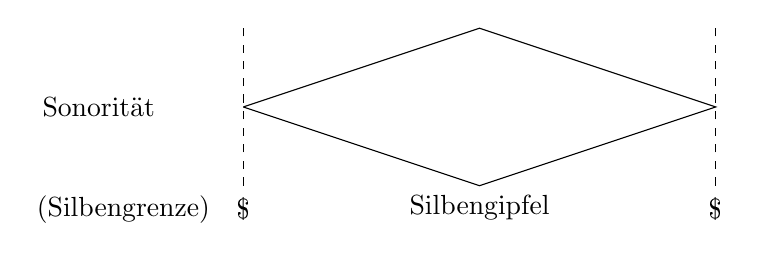
\begin{tikzpicture}
	\draw[dashed] (-3,0)--(-3,2);
	\draw[dashed] (3,0)--(3,2);
	\draw[black] (-3,1)--(0,2)--(3,1)--(0,0)--(-3,1);
	\node at (-3,-0.3){\$};
	\node at (3,-0.3){\$};
	\node[left] at (-3.3,-0.3){(Silbengrenze)};
	\node[left] at (-4,1){Sonorität};
	\node[below] at (0,0){Silbengipfel};
	\end{tikzpicture}
	\caption{Sonoritätsskala in \citet[19]{Lenerz85a}} %\citet[93]{Ramers08a}
\end{figure}
% Vokale sind sonorste Elemente
% m > p
% s > p  (frikativ > plosiv)

\begin{itemize}
	\item Laute können nach der Sonoritätshierarchie auf einer Skala (nach ihrer \textbf{Sonorität}) angeordnet werden.
\end{itemize}

\end{frame}


%%%%%%%%%%%%%%%%%%%%%%%%%%%%%%%%%%
\begin{frame}
\frametitle{Varianten der Sonoritätshierarchie}

Es gibt verschiedene Ausformulierungen der Sonoritätshierachie.


\begin{table}
\centering
\begin{tabular}{l|l|l|l|l} 
	 & einfach 				  	 & Hall 					  & \textbf{Wiese} 				& komplex  \\ 
\hline
\hline 
$[+]$& \multirow{6}{*}{Sonorant} & \multirow{2}{*}{Vokal} 	  & \multirow{2}{*}{Vokal} 		& Vokal  \\ 
	 & 							 & 						 	  &								& Vokal (hoch) \\
\cline{3-5}			
	 &							 & \multirow{3}{*}{Liquide}   &								& Gleitlaut \\
	 &						  	 &	 						  & \textipa{/\textscr /}		& Vibrant \\
\cline{4-5}			
	 &						 	 &							  & \textipa{/l/}				& Lateral \\
\cline{3-5}			
	 &							 & Nasal					  & Nasal						& Nasal \\
\hline			
	 &\multirow{6}{*}{Obstruent} & \multirow{6}{*}{Obstruent} & \multirow{3}{*}{Frikativ}	& $[+$sth$]$ Frikativ \\
	 &						 	 &							  &								& $[+$sth$]$ Affrikat \\		
	 &							 &							  &								& $[+$sth$]$ Plosiv \\
\cline{4-5}			
	 &						  	 &							  & \multirow{3}{*}{Plosiv}		& $[-$sth$]$ Frikativ \\
	 &						 	 &							  &								& $[-$sth$]$ Affrikat \\		
$[-]$&							 &							  &								& $[-$sth$]$ Plosiv \\
		
\end{tabular} 

\end{table}

\end{frame}



%%%%%%%%%%%%%%%%%%%%%%%%%%%%%%%%%%

\begin{frame}
%\frametitle{Sonoritätshierarchie}


\begin{block}{Sonoritätsprinzip (Sonority Sequencing Generalization -- SSG)}
In jeder Silbe gibt es ein Segment, das den \textbf{Silbengipfel} bildet, und dem ein oder mehrere Segmente vorangehen und/oder folgen, deren Sonoritätswerte \textbf{zum Silbengipfel hin zunehmen} und \textbf{danach abnehmen}.\\
\hfill (vgl. \citealt[225]{Hall00a}, \citealt[94]{Ramers08a})
\end{block}

\begin{itemize}
	\item Strikt: monoton steigend oder fallend
	\item Abgeschwächt: auch gleichbleibend \citep[vgl.][]{Hall00a}

\end{itemize}


\begin{figure}
	\centering
	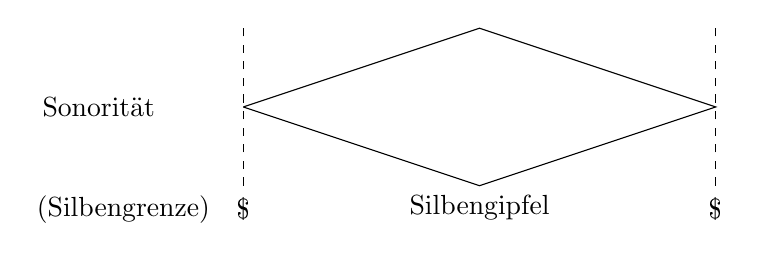
\begin{tikzpicture}
	\draw[dashed] (-3,0)--(-3,2);
	\draw[dashed] (3,0)--(3,2);
	\draw[black] (-3,1)--(0,2)--(3,1)--(0,0)--(-3,1);
	\node at (-3,-0.3){\$};
	\node at (3,-0.3){\$};
	\node[left] at (-3.3,-0.3){(Silbengrenze)};
	\node[left] at (-4,1){Sonorität};
	\node[below] at (0,0){Silbengipfel};
\end{tikzpicture}
	\caption{Sonoritätsskala in \citet[19]{Lenerz85a}} %\citet[93]{Ramers08a}
\end{figure}


\end{frame}


%%%%%%%%%%%%%%%%%%%%%%%%%%%%%%%%%%
\begin{frame}
%\frametitle{Sonoritätshierarchie}

\begin{block}{Sonoritätshierarchie (für uns)}
Vokal $>$ \textipa{/\textscr /} $>$ \textipa{/l/} $>$ Nasal $>$ Frikativ $>$ Plosiv \\
$x > y$ $:=$ $x$ ist sonorer als $y$
\end{block}

\begin{figure}
	\centering
	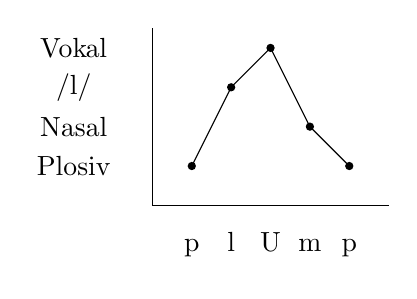
\begin{tikzpicture}[scale=0.5]
	\draw[black] (-1,0) -- (5,0) ; % x axis
	\draw[black] (-1,0) -- (-1,4.5); % y axis
	\node at (-3,1) {Plosiv};
	\node at (-3,2) {Nasal};
	\node at (-3,3) {\textipa{/l/}};
	\node at (-3,4) {Vokal};
	\draw[black] (0,1) -- (1,3) -- (2,4) -- (3,2) -- (4,1);
	\node at (0,-1) {\strut \textipa{p}};
	\node at (1,-1) {\strut \textipa{l}};
	\node at (2,-1) {\strut \textipa{U}};
	\node at (3,-1) {\strut \textipa{m}};
	\node at (4,-1) {\strut \textipa{p}};
	\fill (0,1) circle [radius=3pt];
	\fill (1,3) circle [radius=3pt];
	\fill (2,4) circle [radius=3pt];
	\fill (3,2) circle [radius=3pt];
	\fill (4,1) circle [radius=3pt];
	\end{tikzpicture}
\caption{\citep[225]{Hall00a}}
\end{figure}


%\begin{figure}
%\centering
%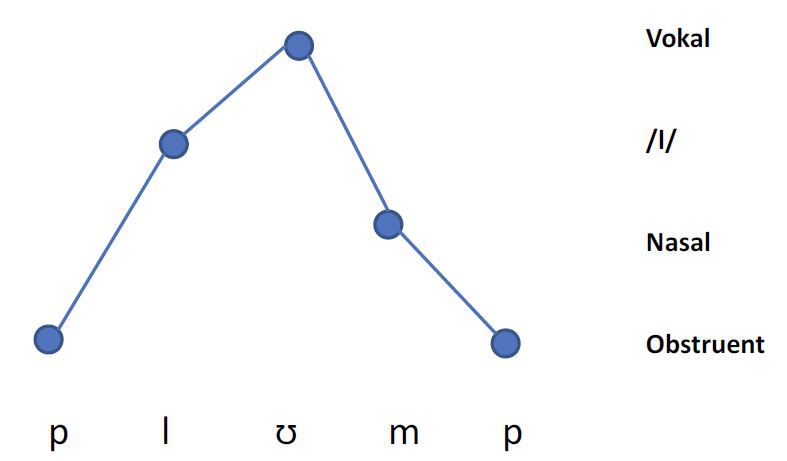
\includegraphics[scale=.3]{material/03bSonoritaetBsp}
%\caption{\citet[225]{Hall00a}}
%\end{figure}

\begin{itemize}
	\item Sonoritätshierarchie wird je nach Sprache leicht anders spezifiziert.
\end{itemize}
\end{frame}


%%%%%%%%%%%%%%%%%%%%%%%%%%%%%%%%%%
\begin{frame}
\frametitle{Übung}

\begin{itemize}
	\item Geben Sie die Sonoritätsprofile der folgenden Silben an.
	
	\ea Spatz, Dachs, Clown, Milch
	\z
	
	% bei Spatz geht es von Frikativ s auf Plosiv p runter = Ausnahme
	% bei Dachs geht es auf k runter und dann auf s hoch   = Ausnahme
	% clown k = plosiv, l = /l/ au = Vokal, n = , keine Ausnahme
	
	% Glottal stop gehört zu den Plosiven
	
	\item Erklären Sie die Ungrammatikalität der folgenden Silben:
	
	\begin{exe}
	\ex \label{ex:lbat}
	\begin{xlist}
		\ex [*]{\textipa{[lbat]}}
		\ex [*]{\textipa{[blabl]}}
		\ex [*]{\textipa{[ki:l\textscr]}}
		\ex [*]{\textipa{[ngang]}}
		\ex [*]{\textipa{[krafm]}}
		\ex [*]{\textipa{[elat]}}
		\ex [*]{\textipa{[plaml]}}
		\ex [*]{\textipa{[nfatl]}}
	\end{xlist}
\end{exe}
	
\end{itemize}

\end{frame}


%%%%%%%%%%%%%%%%%%%%%%%%%%%%%%%%%%%
\iftoggle{ue-loesung}{
	%%%%%%%%%%%%%%%%%%%%%%%%%%%%%%%%%%
%% UE 1 - 03b Phonologie
%%%%%%%%%%%%%%%%%%%%%%%%%%%%%%%%%%

\begin{frame}
\frametitle{Übung: Sonoritätsprofile -- Lösung}

\vfill
\hfill
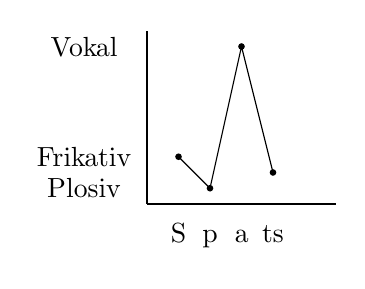
\begin{tikzpicture}[scale=0.4]
\draw[black] (-1,0) -- (5,0) ; % x axis
\draw[black] (-1,0) -- (-1,5.5); % y axis
\node at (-3,0.5) {Plosiv};
\node at (-3,1.5) {Frikativ};
\node at (-3,5) {Vokal};
\draw[black] (0,1.5) -- (1,0.5) -- (2,5) -- (3,1);
\node at (0,-1) {\strut \textipa{S}};
\node at (1,-1) {\strut \textipa{p}};
\node at (2,-1) {\strut \textipa{a}};
\node at (3,-1) {\strut \textipa{\texttoptiebar{ts}}};
\fill (0,1.5) circle [radius=3pt];
\fill (1,0.5) circle [radius=3pt];
\fill (2,5) circle [radius=3pt];
\fill (3,1) circle [radius=3pt];
\end{tikzpicture}
\pause
\hfill
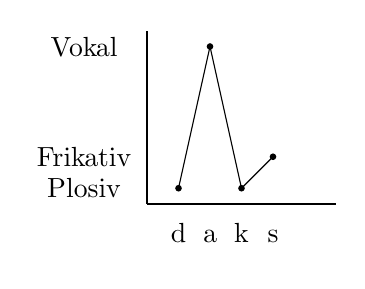
\begin{tikzpicture}[scale=0.4]
\draw[black] (-1,0) -- (5,0) ; % x axis
\draw[black] (-1,0) -- (-1,5.5); % y axis
\node at (-3,0.5) {Plosiv};
\node at (-3,1.5) {Frikativ};
\node at (-3,5) {Vokal};
\draw[black] (0,0.5) -- (1,5) -- (2,0.5) -- (3,1.5);
\node at (0,-1) {\strut \textipa{d}};
\node at (1,-1) {\strut \textipa{a}};
\node at (2,-1) {\strut \textipa{k}};
\node at (3,-1) {\strut \textipa{s}};
\fill (0,0.5) circle [radius=3pt];
\fill (1,5) circle [radius=3pt];
\fill (2,0.5) circle [radius=3pt];
\fill (3,1.5) circle [radius=3pt];
\end{tikzpicture}
\hfill\mbox{}
\vfill
\pause
\hfill
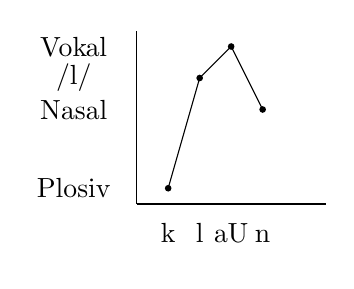
\begin{tikzpicture}[scale=0.4]
\draw[black] (-1,0) -- (5,0) ; % x axis
\draw[black] (-1,0) -- (-1,5.5); % y axis
\node at (-3,0.5) {Plosiv};
\node at (-3,3) {Nasal};
\node at (-3,4) {\textipa{/l/}};
\node at (-3,5) {Vokal};
\draw[black] (0,0.5) -- (1,4) -- (2,5) -- (3,3);
\node at (0,-1) {\strut \textipa{k}};
\node at (1,-1) {\strut \textipa{l}};
\node at (2,-1) {\strut \textipa{\texttoptiebar{aU}}};
\node at (3,-1) {\strut \textipa{n}};
\fill (0,0.5) circle [radius=3pt];
\fill (1,4) circle [radius=3pt];
\fill (2,5) circle [radius=3pt];
\fill (3,3) circle [radius=3pt];
\end{tikzpicture}
\hfill
\pause
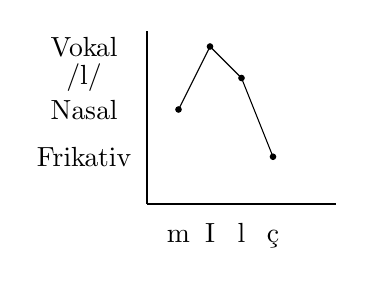
\begin{tikzpicture}[scale=0.4]
\draw[black] (-1,0) -- (5,0) ; % x axis
\draw[black] (-1,0) -- (-1,5.5); % y axis
\node at (-3,1.5) {Frikativ};
\node at (-3,3) {Nasal};
\node at (-3,4) {\textipa{/l/}};
\node at (-3,5) {Vokal};
\draw[black] (0,3) -- (1,5) -- (2,4) -- (3,1.5);
\node at (0,-1) {\strut \textipa{m}};
\node at (1,-1) {\strut \textipa{I}};
\node at (2,-1) {\strut \textipa{l}};
\node at (3,-1) {\strut \textipa{\c{c}}};
\fill (0,3) circle [radius=3pt];
\fill (1,5) circle [radius=3pt];
\fill (2,4) circle [radius=3pt];
\fill (3,1.5) circle [radius=3pt];
\end{tikzpicture}
\hfill\mbox{}
\vfill
\end{frame}


%%%%%%%%%%%%%%%%%%%%%%%%%%%%%%%%%%
\begin{frame}
\frametitle{Übung -- Lösung}

\begin{itemize}
\item Erklären Sie die Ungrammatikalität der folgenden Silben:\\
(Vokal $>$ \textipa{/\textscr /} $>$ \textipa{/l/} $>$ Nasal $>$ Frikativ $>$ Plosiv)
\begin{exe}
	\exr{ex:lbat}
	\settowidth\jamwidth{XXXXXXXXXXXXXXXXXXXXXXXXXXXXXXXXXX}
	\begin{xlist}
		\ex[*]{ \textipa{[lbat]}\loesung{2}{\textipa{[l]} vor \textipa{[b]} im Onset} }
		\ex[*]{ \textipa{[blabl]}\loesung{3}{\textipa{[b]} vor \textipa{[l]} in der Koda $+$ Auslautverhärtung} }
		\ex[*]{ \textipa{[{\textscr}mapt]}\loesung{4}{\textipa{[\textscr ]}vor \textipa{[m]} im Onset } }
		\ex[*]{ \textipa{[ki:l\textscr]}\loesung{5}{\textipa{[l]} vor \textipa{[\textscr ]} in der Koda} }
		\ex[*]{ \textipa{[ngang]}\loesung{6}{\textipa{[n]} vor \textipa{[g]} im Onset $+$ reg. velare Nasalassimiliation } \loesung{6}{$+$ g-Tilgung}}
		\ex[*]{ \textipa{[krafm]}\loesung{7}{\textipa{[f]} vor \textipa{[m]} in der Koda} }
		\ex[*]{ \textipa{[elat]}\loesung{8}{2 Silben (2 Nuklei) $+$ Knacklauteinsetzung} }
		\ex[*]{ \textipa{[plaml]}\loesung{9}{\textipa{[m]} vor \textipa{[l]} in der Koda} }
		\ex[*]{ \textipa{[nfatl]}\loesung{10}{\textipa{[n]} vor \textipa{[f]} im Onset $+$ \textipa{[t]} vor \textipa{[l]} in der Koda} }
	\end{xlist}
\end{exe}

\end{itemize}

\end{frame}


}
%%%%%%%%%%%%%%%%%%%%%%%%%%%%%%%%%%

\subsubsection{Weitere phonotaktische Beschränkungen}

%%%%%%%%%%%%%%%%%%%%%%%%%%%%%%%%%%

\begin{frame}
\frametitle{Weitere phonotaktische Beschränkungen}

\begin{columns}
	
	\column{.6\textwidth}	
\begin{itemize}
	\item Im \textbf{Onset} in deutschen Silben können stehen:
	
	\begin{itemize}
		\item alle Einzelkonsonanten des Deutschen 
		
		(\textbf{außer} \textipa{[N]} und \textipa{[s]} vor Vokal am Wortanfang)

		\item bestimmte zwei- und dreigliedrige Konsonantencluster nach Sonoritätshierarchie
		
		\item bestimmte zweigliedrige Konsonantencluster\\
		 (s. Tabelle: von links nach oben im Onset, in der Koda umgekehrt, \citealp[vgl.][231-235]{Hall00a})
	\end{itemize}

	\ea *\textipa{[fma]} \vs \textipa{[fla]}
	\ex *\textipa{[lpa]} \vs \textipa{[pla]}
	\ex *\textipa{[mSa]} \vs \textipa{[Sma]}
	\ex *\textipa{[m\;Ra]}
	\z
\end{itemize}
	
	\column{.35\textwidth}
\begin{table}
	\centering
	
	\begin{tabular}{c|c|c|c|c}
		& \textipa{m} & \textipa{n} & \textipa{l} & \textipa{\textscr} \\ 
		\hline 
		\textipa{p} &  &  & $+$ & $+$ \\ 
		\hline 
		\textipa{b} &  &  & $+$ & $+$ \\ 
		\hline 
		\textipa{t} &  &  &  & $+$ \\ 
		\hline 
		\textipa{d} &  &  &  & $+$ \\ 
		\hline 
		\textipa{k} &  & $+$ & $+$ & $+$ \\ 
		\hline 
		\textipa{g} &  & $+$ & $+$ & $+$ \\ 
		\hline 
		\textipa{f} &  &  & $+$ & $+$ \\
		\hline 
		\textipa{v} &  &  &  & $+$ \\ 
		\hline 
		\textipa{S} & $+$ & $+$ & $+$ & $+$ \\ 
	\end{tabular} 
	
	\caption{Kombinatorik von Sonoranten mit Obstruenten im Deutschen}
\end{table}

\end{columns}	

\end{frame}	
%%%%%%%%%%%%%%%%%%%%%%%%%%%%%%%%%

\begin{frame}{Weitere phonotaktische Beschränkungen}
	
\begin{itemize}	
	\item Silben können auch \textbf{mit unbetontem Vokal} beginnen (\ras leerer Onset).
	\ea \ab{Eier}: \textipa{[\textprimstress P\t{aɪ}.\alertred{5}]}
	\z
	
	\ea \ab{etwaig}: \textipa{[PEt.\textprimstress va:.\alertred{I}\c{c}]} 
	\z

\pause 
	
	\item Vor betontem Vokal steht immer ein Konsonant (\textbf{Glottisschlag}).
	
	\ea
	\textipa{[ka.\alertred{\textprimstress Po:}.tIS]}
	\z

\end{itemize}

\end{frame}


%%%%%%%%%%%%%%%%%%%%%%%%%%%%%%%%%%
\subsection{Hausaufgabe}
%%%%%%%%%%%%%%%%%%%%%%%%%%%%%%%%%%

\begin{frame}
\frametitle{Hausaufgabe}

\begin{itemize}
	\item[1.]{Geben Sie die standarddeutsche \textbf{phonetische Transkription} für folgende Wörter an:}
	
	\eal \label{ex:03bHA1}
	\ex Spitzenschuhe
	\ex Endausscheidung
	\ex Platzanweiser
	\ex verzweifeln
	\ex abverlangen
	\ex Überarbeitung
	\ex Zugeständnis
	\zl
\end{itemize}

\end{frame}
%%%%%%%%%%%%%%%%%%%%%%%%%%%%%%%%%

\begin{frame}{Hausaufgabe}

\begin{itemize}
\item[2.]{Erläutern Sie anhand der folgenden Beispiele, unter welchen Bedingungen die \textbf{Auslautverhärtung} im Deutschen stattfindet.}

\eal \label{ex:03bHA2}
\ex Wand -- Wände
\ex lesen -- lesbar
\ex sagen -- sagst
\ex Roggen
\zl

\end{itemize}

\end{frame}
%%%%%%%%%%%%%%%%%%%%%%%%%%%%%%%%%%

\begin{frame}{Hausaufgabe}

\begin{itemize}
\item[3.]{Geben Sie fünf verschiedene \textbf{phonetische oder phonologische Prozesse} an, die in dem folgenden Satz -- teilweise nur bei schnellerem Sprechen -- beobachtet werden können.} 

\ea \label{ex:03bHA3}
\begin{quote}
Um die fünf Haken in regelmäßigen Abständen an die Wand schrauben zu können, sollten Sie sich Bohrmaschine, Wasserwaage, Zollstock und Dübel bereitgelegt haben und auf keinen Fall die Nerven verlieren, bevor Sie nicht befestigt sind.
\end{quote}
\z

\end{itemize}

\end{frame}
%%%%%%%%%%%%%%%%%%%%%%%%%%%%%%%%%%%

\begin{frame}{Hausaufgabe}

\begin{itemize}	
\item[4.]{Illustrieren Sie den deutschen phonemischen Kontrast der folgenden Phoneme durch
  \textbf{Minimalpaare}, wobei der Kontrast (wenn möglich) ein Mal initial,\\
ein Mal final vorkommen soll.

Beispiel: \textipa{[p]} -- \textipa{[f]} Paul -- faul (Initialposition), Laub -- Lauf (Finalposition)}

\eal \label{ex:03bHA4}
\ex \textipa{[m]} -- \textipa{[n]}
\ex \textipa{[p]} -- \textipa{[b]}
\ex \textipa{[h]} -- \textipa{[v]}
\ex \textipa{[n]} -- \textipa{[N]}
\ex \textipa{[f]} -- \textipa{[v]}
\zl

\end{itemize}
\end{frame}


%%%%%%%%%%%%%%%%%%%%%%%%%%%%%%%%%%%
\iftoggle{ha-loesung}{
	%%%%%%%%%%%%%%%%%%%%%%%%%%%%%%%%%%
%% HA 1 - 03b Phonologie
%%%%%%%%%%%%%%%%%%%%%%%%%%%%%%%%%%

\begin{frame}
\frametitle{Hausaufgabe -- Lösung}

\begin{itemize}
	\item[1.]{Geben Sie die standarddeutsche \textbf{phonetische Transkription} für folgende Wörter an:}
	
	\begin{exe}
		\exr{ex:03bHA1}
		\begin{xlist}
		\settowidth\jamwidth{XXXXXXXXXXXXXXXXXXXXXXXXXXXXXX}
			\ex Spitzenschuhe \loesung{2}{\textipa{['SpI\textsubdot{\t{ts}}@n.Su:.@]}}
			\ex Endausscheidung \loesung{3}{\textipa{['PEnt.P\texttoptiebar{aU}s.S\texttoptiebar{aI}.dUN]}}
			\ex Platzanweiser \loesung{4}{\textipa{['pla\texttoptiebar{ts}.Pan.v\texttoptiebar{aI}.z5]}}
			\ex verzweifeln \loesung{5}{\textipa{[fE5.'\texttoptiebar{ts}v\texttoptiebar{aI}.f@ln]}}
			\ex abverlangen \loesung{6}{\textipa{['Pap.fE5.la\.N@n]}}
			\ex Überarbeitung \loesung{7}{\textipa{[Py:.b5.'Pa\;R.b\texttoptiebar{aI}.tUN]}}
			\ex Zugeständnis \loesung{8}{\textipa{['\texttoptiebar{ts}u:.g@.StEnt.nIs]}}
		\end{xlist}
	\end{exe}

\end{itemize}

\end{frame}
%%%%%%%%%%%%%%%%%%%%%%%%%%%%%%%%%

\begin{frame}{Hausaufgabe -- Lösung}

\begin{itemize}
	\item[2.]{Erläutern Sie anhand der folgenden Beispiele, unter welchen Bedingungen die \textbf{Auslautverhärtung} im Deutschen stattfindet.}

	\begin{exe}
		\exr{ex:03bHA2}
		\begin{xlist}
		\settowidth\jamwidth{XXXXXXXXXXXXXXXXXXXXXXXXXXXXXXX}
			\ex Wand -- Wände \loesung{2}{sth. Plosive am Wortende}
			\ex lesen -- lesbar \loesung{3}{generell am Silbenende}
			\ex sagen -- sagst \loesung{4}{betrifft \emph{alle} sth. Plosive in der Koda}
			\ex Roggen \loesung{5}{jedoch keine Silbengelenke}
		\end{xlist}
	\end{exe}

\end{itemize}

\end{frame}


%%%%%%%%%%%%%%%%%%%%%%%%%%%%%%%%%%
\begin{frame}{Hausaufgabe -- Lösung}

\begin{itemize}
\item[3.]{Geben Sie fünf verschiedene \textbf{phonetische oder phonologische Prozesse} an, die in dem folgenden Satz -- teilweise nur bei schnellerem Sprechen -- beobachtet werden können.} 

\begin{exe}
	\exr{ex:03bHA3}
	\begin{quote}
	Um die fünf Haken in regelmäßigen Abständen an die Wand schrauben zu können, sollten Sie sich Bohrmaschine, Wasserwaage, Zollstock und Dübel bereitgelegt haben und auf keinen Fall die Nerven verlieren, bevor Sie nicht befestigt sind.
	\end{quote}
\end{exe}


\begin{description}
	\item[\alertgreen{\textbf{Beispiele:}}] ~

\alertgreen{
	regressive Nasalassimilation in \emph{fünf}: \textipa{[fY\textbf{m}f]}\\
	progressive Nasalassimilation nach Schwa-Elision (feeding) in \emph{Haken}: \textipa{[hak\textbf{N}]}\\
	Auslautverhärtung in \emph{Wand}: \textipa{[van\textbf{t}]}\\
	progressive Nasalassimilation nach Schwa-Elision (feeding) in \emph{schrauben}: \textipa{[S\;R\t{aU}b\textbf{m}]}\\
	g-Spirantisierung in \emph{befestigt}: \textipa{[b@fEstI\textbf{\c{c}}t]}\\
	r-Vokalisierung in \emph{Bohrmaschine}: \textipa{[bo\textbf{5}maSi:n@]}
}						
		\end{description}

\end{itemize}

\end{frame}


%%%%%%%%%%%%%%%%%%%%%%%%%%%%%%%%%%%
\begin{frame}{Hausaufgabe -- Lösung}

\begin{itemize}	
\item[4.]{Illustrieren Sie den deutschen phonemischen Kontrast der folgenden Phoneme durch \textbf{Minimalpaare}, wobei der Kontrast (wenn möglich) ein Mal initial, ein Mal final vorkommen soll.

Beispiel: \textipa{[p]} -- \textipa{[f]} Paul -- faul (Initialposition), Laub -- Lauf (Finalposition)}

\begin{exe}
	\exr{ex:03bHA4}
	\settowidth\jamwidth{XXXXXXXXXXXXXXXXXXXXXXXXXXXXXXXXXXXX}
	\begin{xlist}
		\ex \textipa{[m]} -- \textipa{[n]} \loesung{2}{muss -- Nuss, beim -- Bein}
		\ex \textipa{[p]} -- \textipa{[b]} \loesung{3}{Pass -- Bass}
			\loesung{3}{(wegen Auslautverhärtung kein finaler Kontrast möglich)}
		\ex \textipa{[h]} -- \textipa{[v]} \loesung{4}{heiß -- weiß (\textipa{[h]} kommt nicht final vor)}
		\ex \textipa{[n]} -- \textipa{[N]} \loesung{5}{Sinn -- sing (\textipa{[N]} kommt nicht initial vor)}
		\ex \textipa{[f]} -- \textipa{[v]} \loesung{6}{Fass -- was}
			\loesung{6}{(wegen Auslautverhärtung kein finaler Kontrast möglich)}
	\end{xlist}
\end{exe}
		
\end{itemize}

\end{frame}
}
%%%%%%%%%%%%%%%%%%%%%%%%%%%%%




%@EE: Checken: Keine Abbildungen und elektronischen Quellen?



%%%%%%%%%%%%%%%%%%%%%%%%%%%%%%%%%%%%%%%%%%%%%%%%
%% Compile the master file!
%% 		Include: Stefan Müller
%% 		Course: GK Linguistik
%%%%%%%%%%%%%%%%%%%%%%%%%%%%%%%%%%%%%%%%%%%%%%%%

%\exewidth{(35)} im übergeordneten File

% sollte zentral geladen werden. St. Mü. 04.11.2016 (in localcommands?)
%%%%%%%%%%%%%
%%% Forestset Syllables

\newbox\foreststrutbox
\setbox\foreststrutbox=\hbox to 0pt{\phantom{\forestOve{standard node}{content}}}
\def\foreststrut{\copy\foreststrutbox}
\forestset{
GP1/.style 2 args={
for n={1}{baseline},
s sep=0pt, l sep=0pt,
for descendants={
l sep=0pt, l={#1},
anchor=base,calign=first,child anchor=north,
inner xsep=1pt,inner ysep=2pt,outer sep=0pt,s sep=0pt,
},
delay={
if content={}{phantom}{for children={no edge}},
for tree={
if content={O}{tier=OR}{},
if content={R}{tier=OR}{},
if content={N}{tier=N}{},
if content={x}{
tier=x,content={$\times$},outer xsep={#2},
for tree={calign=center},
for descendants={content format={\foreststrut\forestoption{content}}},
before drawing tree={outer xsep=0pt,delay={typeset node}},
s sep=4pt
}{},
},
},
before drawing tree={where content={}{parent anchor=center,child anchor=center}{}},
},
GP1/.default={5ex}{8.0pt},
associate/.style={%
tikz+={\draw(!)--(!#1);}},
spread/.style={
before drawing tree={tikz+={\draw[dotted](!)--(!#1);}}},
govern/.style={
before drawing tree={tikz+={\draw[->](!)--(!#1);}}},
p-govern/.style={
before drawing tree={tikz+={\draw[->](.north) to[out=150,in=30] (!#1.north);}}},
no p-govern/.style={
before drawing tree={tikz+={\draw[->,loosely dashed](.north) to[out=150,in=30] (!#1.north);}}},
encircle/.style={before drawing tree={circle,draw,inner sep=0pt}},
fen/.style={pin={[font=\footnotesize,inner sep=1pt,pin edge=<-]10:\textsc{Fen}}},
el/.style={content=\textsc{\textbf{##1}}},
head/.style={content=\textsc{\textbf{\underline{##1}}}},
llap/.style={
tikz+={%
\edef\forest@temp{\noexpand\node[\option{node options},
anchor=base east,at=(.base east)]}%
\forest@temp{#1\phantom{\option{environment}}};
}
},
rlap/.style={
tikz+={%
\edef\forest@temp{\noexpand\node[\option{node options},
anchor=base west,at=(.base west)]}%
\forest@temp{\phantom{\option{environment}}#1};
}
},
}
%%%%%%%%%%%%%


%%%%%%%%%%%%%%%%%%%%%%%%%%%%%%%%%%%%%%%%%%%%%%%%%%%%
%%%             Metadata                         
%%%%%%%%%%%%%%%%%%%%%%%%%%%%%%%%%%%%%%%%%%%%%%%%%%%% 

\title{Grundkurs Linguistik}

\subtitle{Phonologie III: Silbenmodelle}

\author[St. Mü.]{
	{\small Stefan Müller}
	\\
	{\footnotesize \url{http://www.linguistik.hu-berlin.de/staff/amyp}}
	%	\\
	%	{\small\href{mailto:mapriema@hu-berlin.de}{mapriema@hu-berlin.de}}
}

\institute{Institut für deutsche Sprache und Linguistik}

% bitte lassen, sonst kann man nicht sehen, von wann die PDF-Datei ist.
%\date{ }

%\publishers{\textbf{6. linguistischer Methodenworkshop \\ Humboldt-Universität zu Berlin}}

%\hyphenation{nobreak}


%%%%%%%%%%%%%%%%%%%%%%%%%%%%%%%%%%%%%%%%%%%%%%%%%%%%
%%%             Preamble's End                  
%%%%%%%%%%%%%%%%%%%%%%%%%%%%%%%%%%%%%%%%%%%%%%%%%%%%   


%%%%%%%%%%%%%%%%%%%%%%%%%   
\huberlintitlepage[22pt]
\iftoggle{toc}{
\frame{
%\begin{multicols}{2}
	\frametitle{Inhaltsverzeichnis}
	\tableofcontents
	%[pausesections]
%\end{multicols}
}
}

%%%%%%%%%%%%%%%%%%%%%%%%%%%%%%%%%%
%%%%%%%%%%%%%%%%%%%%%%%%%%%%%%%%%%
%%%%%LITERATURE:

%% Allgemein
\nocite{Glueck&Roedel16a}
\nocite{Schierholz&Co18}
\nocite{Luedeling2009a}
\nocite{Meibauer&Co07a} 
\nocite{Repp&Co15a} 

%%% Sprache & Sprachwissenschaft
%\nocite{Fries16c} %Adäquatheit
%\nocite{Fries16a} %Grammatikalität
%\nocite{Fries&MyP16c} %GG
%\nocite{Fries&MyP16b} %Akzeptabilität
%\nocite{Fries&MyP16d} %Kompetenz vs. Performanz

%% Phonetik & Phonologie
\nocite{Altmann&Co07a}
\nocite{DudenAussprache00a}
\nocite{Hall00a} 
\nocite{Kohler99a}
\nocite{Krech&Co09a}
\nocite{Pompino95a}
\nocite{Ramers08a}
\nocite{Ramers&Vater92a}
\nocite{Rues&Co07a}
\nocite{WieseR96a}
\nocite{WieseR11a}


%%%%%%%%%%%%%%%%%%%%%%%%%%%%%%%%%%
%%%%%%%%%%%%%%%%%%%%%%%%%%%%%%%%%%
\section{Phonologie III: Silbenmodelle}
%%%%%%%%%%%%%%%%%%%%%%%%%%%%%%%%%%
\begin{frame}
\frametitle{Begleitlektüre}

\begin{itemize}
	\item \textbf{obligatorisch:}
	\begin{itemize}
		\item[] AM S.~24--30
		\item[] \citet{Hall00a}: Kapitel~2 (S.~47--62)
	\end{itemize}
	\item \textbf{optional:}
	\begin{itemize}
		\item[] \citet{Hall00a}: Kapitel~8 (S.~238--254)
	\end{itemize}
\end{itemize}

\end{frame}


%%%%%%%%%%%%%%%%%%%%%%%%%%%%%%%%%%
%%%%%%%%%%%%%%%%%%%%%%%%%%%%%%%%%%
\subsection{Silbenmodelle}

%% MyP: Contents
\iftoggle{sectoc}{
	\frame{
		%\begin{multicols}{2}
		\frametitle{~}
		\tableofcontents[currentsubsection, subsubsectionstyle=hide]
		%\end{multicols}
	}
}

%% StM: Contents
\iftoggle{gliederung}{
	
	\outline{
		\begin{itemize}
			
			\item \blaubf{Silbenmodelle}
			%% CV-Modell
			%% Konstituentenmodell
			\item Silbengelenk
			\item Silbifizierung
			\item Exkurs: Akzent
			\item Hausaufgabe
			
		\end{itemize}
	}
}
%%%%%%%%%%%%%%%%%%%%%%%%%%%%%%%%%%

\begin{frame}
\frametitle{Silbenmodelle}

\begin{itemize}
	\item Bisher (hauptsächlich) nur \textbf{lineare Betrachtung} mit allen Segmenten auf einer Schicht
	\ea
	\textipa{/pe:.t@\textscr /} (Peter)
	\z
	
	\ea
	\textipa{/vE\.t@\textscr /} (Vetter)
	\z
	
	\item \textbf{Nicht-lineare Phonologie} (Autosegmentale Phonologie)
	
	\begin{itemize}
		\item verschiedene Repräsentationsebenen bzw. Schichten
		
		\item hierarchische Strukturierung
		
		\item Vorteil: 
		
		Beschreibung von \textbf{Merkmalsausbreitung} und \textbf{segmentunabhängigen Prozessen}
		
	\end{itemize}
\end{itemize}

\end{frame}


%%%%%%%%%%%%%%%%%%%%%%%%%%%%%%%%%%
%%%%%%%%%%%%%%%%%%%%%%%%%%%%%%%%%%
\subsubsection{CV-Modell}
%\frame{
%\frametitle{~}
%	\tableofcontents[currentsection]
%}
%%%%%%%%%%%%%%%%%%%%%%%%%%%%%%%%%%

\begin{frame}%[shrink]
\frametitle{CV-Modell (einfaches Modell)}

\begin{itemize}
\item Silben und Segmente auf unterschiedlichen Schichten

\item verbunden durch Assoziationslinien

\item Charakterisierung der Silbenstruktur durch C und V 
\end{itemize}

\begin{columns}
	
\column[c]{.45\textwidth}
\begin{figure}
	\centering
	\begin{forest}
		MyP edges,
		[$\sigma$
		[C [\textipa{b}]]
		[C [\textipa{l}]]
		[V [\textipa{I}]]
		[C [\textipa{n}]]
		[C [\textipa{t}]]
		]
	\end{forest}
	\caption{CV-Modell}
\end{figure}


\column[c]{.5\textwidth}
$\sigma :=$ Silbe

C $:=$ nicht-silbisch, \gqq{konsonantisch}

V $:=$ silbisch, \gqq{vokalisch}

\end{columns}

\end{frame}


%%%%%%%%%%%%%%%%%%%%%%%%%%%%%%%%%%
\begin{frame}
\frametitle{Verteilung von Segmenten in der Silbe}

\begin{itemize}
\item Wie ist die Verteilung von Segmenten in der deutschen Silbe?
\end{itemize}

\begin{minipage}{.59\textwidth}
	\begin{itemize}
	\item C $\neq$ Konsonant, sondern \alertred{nicht-silbisch}
	
	\item V $\neq$ Vokal, sondern \alertblue{silbisch}
	
	\item Jede Silbe enthält \alertgreen{einen Kern} (V).
	\end{itemize}
\end{minipage}
%
\begin{minipage}{.4\textwidth}

\begin{figure}
%\tiny
\small
\centering
\begin{forest}
	MyP edges,
	[$\sigma$
	[C [\textipa{g}]]
	[C [\textipa{l}]]
	[\alertgreen{V} [\textipa{a}]]	
	[C [\alertred{\textipa{U}}]]
	[C [\textipa{p}]]
	[C [\textipa{t}]]
	]
\end{forest}

\begin{forest}
	MyP edges,
	[,phantom
	[$\sigma$
	[C [\textipa{k}]]
	[\alertgreen{V} [\textipa{U}]]
	[C [\textipa{m}]]
	]
	[$\sigma$	
	[C [\textipa{p}]]
	[\alertgreen{V} [\alertblue{\textipa{\textsyllabic{l}}}]]
	]
	]
\end{forest}

\end{figure}

\end{minipage}

% u bei glaubt ist ein C, weil nur a der Silbengipfel ist, u ist weniger sonor, und Diphtonge gelten
% als zwei Zeiteinheiten, bei langen Vokalen wird auch auf zwei geteilt. Der Doppelpunkt ist dann
% ein C

% Bei Beirisch guot geht der Sonoritätsgipfel aufs o und dann ist das o V und davor ein C

\end{frame}


%%%%%%%%%%%%%%%%%%%%%%%%%%%%%%%%%%
\begin{frame}
\frametitle{Verteilung von Segmenten in der Silbe}


\begin{minipage}{.59\textwidth}
	\begin{itemize}
	\item \textbf{maximale Anzahl an Cs} vor und nach V
	
	% Aber strumpfst. Es kommt ein weiteres verbessertes Modell
	
	\item Korrelation zwischen Anzahl an Cs nach V und der \textbf{Länge}/(Un-)Gespanntheit des
          Vokals:\\
              normalerweise nach Lnagvokal kein Konsonantencluster
	\end{itemize}
\end{minipage}
%
\begin{minipage}{.4\textwidth}

\begin{figure}
	%\tiny
	\small
	\centering
	\begin{forest}
	MyP edges,
	[$\sigma$
	[C [\textipa{g}]]
	[C [\textipa{l}]]
	[V [\textipa{a}]]	
	[\alertred{C} [\textipa{U}]]
	[\alertred{C} [\textipa{p}]]
	[\alertred{C} [\textipa{t}]]
	]
	\end{forest}
	
	\begin{forest}
	MyP edges,
	[$\sigma$
	[C [\textipa{k}]]
	[C [\textipa{\textscr }]]
	[V [\textipa{a}]]
	[C [\textipa{N}]]
	[C [\textipa{k}]]	
	]
	\end{forest}

\end{figure}

\end{minipage}

% Kopf pf ist ein C
% Kumpel fällt das e weg und wir haben einen vokalischen Konsonant l

\end{frame}



%%%%%%%%%%%%%%%%%%%%%%%%%%%%%%%%%%
\begin{frame}
\frametitle{Verteilung von Segmenten in der Silbe}


\begin{columns}

\column[t]{.49\textwidth}	
	\begin{itemize}
		\item Diphthonge: \textbf{VC} (bzw. CV \textipa{[g\textsubarch{U}Ot]})
	
		\item lange Vokale: \textbf{VC}
	\end{itemize}

\column[t]{.49\textwidth}
	\begin{itemize}
		\item Affrikate: \textbf{C}
	
		\item silbische Konsonanten: \textbf{V}
	\end{itemize}
\end{columns}


\begin{minipage}{.49\textwidth}

	\begin{figure}
%	\tiny
%	\scriptsize
	\small
	\centering
	\begin{forest}
		MyP edges,
		[$\sigma$
		[C [\textipa{g}]]
		[C [\textipa{l}]]
		[V [\alertred{\textipa{a}}]]	
		[C [\alertred{\textipa{U}}]]
		[C [\textipa{p}]]
		[C [\textipa{t}]]
		]
	\end{forest}
	
	\begin{forest}
		MyP edges,
		[$\sigma$
		[C [\textipa{k}]]
		[V [\alertred{\textipa{a}}]]
		[C [\alertred{\textipa{:}}]]	
		[C [\textipa{l}]]
		]
	\end{forest}
	\end{figure}	

\end{minipage}
%
\begin{minipage}{.49\textwidth}

	\begin{figure}
%	\tiny
%	\scriptsize
	\small
	\centering

	\begin{forest}
	MyP edges,
	[$\sigma$
	[C [\textipa{k}]]
	[V [\textipa{O}]]
	[C [\alertred{\textipa{\t{pf}}}]]	
	[C [\textipa{s}]]
	]
	\end{forest}
	
	\begin{forest}
	MyP edges,
	[,phantom
	[$\sigma$
	[C [\textipa{k}]]
	[V [\textipa{U}]]
	[C [\textipa{m}]]	
	]
	[$\sigma$
	[C [\textipa{p}]]
	[V [\alertred{\textipa{\textsyllabic{l}}}]]
	]
	]
	\end{forest}

\end{figure}

\end{minipage}

\end{frame}



%%%%%%%%%%%%%%%%%%%%%%%%%%%%%%%%%%
%%%%%%%%%%%%%%%%%%%%%%%%%%%%%%%%%%
\subsubsection{Konstituentenmodell}
%\frame{
%\begin{multicols}{2}
%\frametitle{~}
%	\tableofcontents[currentsection]
%\end{multicols}
%}
%%%%%%%%%%%%%%%%%%%%%%%%%%%%%%%%%%

\begin{frame}
\frametitle{Konstituentenmodell}

\begin{itemize}
\item Zerlegung in \textbf{silbische Konstituenten}
\item Silbe ($\sigma$) $=$ Onset (O) $+$ Reim (R)
\item Reim (R) $=$ Nukleus (N) $+$ Koda (K)
\item $+$ Skelettschicht (X)
\end{itemize}

% nur x, C und V braucht man nicht mehr, weil N das V (vokalische Element) ist
% x sind die Zeiteinheiten

\begin{figure}
%%%%%%%%%%%%%%
%%% Forestset Syllables

\newbox\foreststrutbox
\setbox\foreststrutbox=\hbox to 0pt{\phantom{\forestOve{standard node}{content}}}
\def\foreststrut{\copy\foreststrutbox}
\forestset{
GP1/.style 2 args={
for n={1}{baseline},
s sep=0pt, l sep=0pt,
for descendants={
l sep=0pt, l={#1},
anchor=base,calign=first,child anchor=north,
inner xsep=1pt,inner ysep=2pt,outer sep=0pt,s sep=0pt,
},
delay={
if content={}{phantom}{for children={no edge}},
for tree={
if content={O}{tier=OR}{},
if content={R}{tier=OR}{},
if content={N}{tier=N}{},
if content={x}{
tier=x,content={$\times$},outer xsep={#2},
for tree={calign=center},
for descendants={content format={\foreststrut\forestoption{content}}},
before drawing tree={outer xsep=0pt,delay={typeset node}},
s sep=4pt
}{},
},
},
before drawing tree={where content={}{parent anchor=center,child anchor=center}{}},
},
GP1/.default={5ex}{8.0pt},
associate/.style={%
tikz+={\draw(!)--(!#1);}},
spread/.style={
before drawing tree={tikz+={\draw[dotted](!)--(!#1);}}},
govern/.style={
before drawing tree={tikz+={\draw[->](!)--(!#1);}}},
p-govern/.style={
before drawing tree={tikz+={\draw[->](.north) to[out=150,in=30] (!#1.north);}}},
no p-govern/.style={
before drawing tree={tikz+={\draw[->,loosely dashed](.north) to[out=150,in=30] (!#1.north);}}},
encircle/.style={before drawing tree={circle,draw,inner sep=0pt}},
fen/.style={pin={[font=\footnotesize,inner sep=1pt,pin edge=<-]10:\textsc{Fen}}},
el/.style={content=\textsc{\textbf{##1}}},
head/.style={content=\textsc{\textbf{\underline{##1}}}},
llap/.style={
tikz+={%
\edef\forest@temp{\noexpand\node[\option{node options},
anchor=base east,at=(.base east)]}%
\forest@temp{#1\phantom{\option{environment}}};
}
},
rlap/.style={
tikz+={%
\edef\forest@temp{\noexpand\node[\option{node options},
anchor=base west,at=(.base west)]}%
\forest@temp{\phantom{\option{environment}}#1};
}
},
}
%%%%%%%%%%%%%

\centering
\scalebox{.8}{
\begin{forest} MyP edges, [,phantom
[$\sigma$
[O[x, tier=word[\textipa{f}]][x, tier=word[\textipa{K}]]]
[R[N[x, tier=word[\textipa{\textopeno}]]][K[x[\textipa{s}]]]]
]
[$\sigma$
[O[x, tier=word[\textipa{t}]]]
[R[N[x[\textipa{I}]]][K[x[\c{c}]]]]
]  
]
\end{forest}}

% frostig
%\caption{Konstituentenmodell}
\end{figure}

\end{frame}



%%%%%%%%%%%%%%%%%%%%%%%%%%%%%%%%%%

\begin{frame}
\frametitle{Silbe, Onset und Reim}

\textbf{Silbe} ($\sigma$) = Onset (O) + Reim (R)

\begin{itemize}
\item \textbf{Onset}: 

	\begin{itemize}
		\item Evidenz aus Versprecherforschung: Onset ist betroffen, nicht der Rest
		
		\ea
		\textipa{\alertred{k}Il\c{c}.\alertblue{m}a\.fe:} vs. \textipa{\alertblue{m}Il\c{c}.\alertred{k}a\.fe:} (nicht \textipa{k\textbf{a}l\c{c}.m\textbf{I}\.fe:})
		\z
		% Versprecher: Kilchmafee für   Milchkafee
		% Aber keinen Versprecher * Kalchmifee
	\end{itemize}	

\pause 

\item \textbf{Reim}: 
	\begin{itemize}
		\item Silbengewicht: Längenausgleich zwischen Nukleus und Koda 		
		% Onset ist für den Längenausgleich irrelevant. wenn Koda lang, dann Nukleus kurz. Findet alles
		% innerhalb des Reims statt
		
		% Auch Auslautverhärtung findet in der Koda statt:
		% sagst -> sakst, d.h. g ist in der Koda
		
		\item Gedichte
		\item typischerweise VCC (auch als VVC kodiert)
	\end{itemize}

\end{itemize}

\textbf{Reim} (R) = Nukleus (N) + Koda (K)

	\begin{itemize}
		\item \textbf{Nukleus}: obligatorischer Bestandteil der Silbe
		
		\item \textbf{Koda}: Regeln, die sich nur auf die Konsonanten in der Koda beziehen
	\end{itemize}

\end{frame}


%%%%%%%%%%%%%%%%%%%%%%%%%%%%%%%%%
\begin{frame}[shrink]
\frametitle{Skelettschicht}

\begin{itemize}
\item Ebene zwischen den Segmenten und den Silbenkonstituenten

\item X $:=$ abstrakte Zeiteinheit (\zB für Darstellung des Längenausgleichs)

\item X \ras vergleichbar mit C und V

\item \textbf{Nukleus}:

\begin{itemize}
\item 1 X: Kurzvokal, silbischer Konsonant
\item 2 X: Langvokal, Diphthong
\item (3 X: Langvokal + vokalisiertes \textipa{/\textscr /} \ras umstritten)
\end{itemize}

\end{itemize}


\begin{minipage}{.325\textwidth}

%%%%%%%%%%%%%%
%%% Forestset Syllables

\newbox\foreststrutbox
\setbox\foreststrutbox=\hbox to 0pt{\phantom{\forestOve{standard node}{content}}}
\def\foreststrut{\copy\foreststrutbox}
\forestset{
GP1/.style 2 args={
for n={1}{baseline},
s sep=0pt, l sep=0pt,
for descendants={
l sep=0pt, l={#1},
anchor=base,calign=first,child anchor=north,
inner xsep=1pt,inner ysep=2pt,outer sep=0pt,s sep=0pt,
},
delay={
if content={}{phantom}{for children={no edge}},
for tree={
if content={O}{tier=OR}{},
if content={R}{tier=OR}{},
if content={N}{tier=N}{},
if content={x}{
tier=x,content={$\times$},outer xsep={#2},
for tree={calign=center},
for descendants={content format={\foreststrut\forestoption{content}}},
before drawing tree={outer xsep=0pt,delay={typeset node}},
s sep=4pt
}{},
},
},
before drawing tree={where content={}{parent anchor=center,child anchor=center}{}},
},
GP1/.default={5ex}{8.0pt},
associate/.style={%
tikz+={\draw(!)--(!#1);}},
spread/.style={
before drawing tree={tikz+={\draw[dotted](!)--(!#1);}}},
govern/.style={
before drawing tree={tikz+={\draw[->](!)--(!#1);}}},
p-govern/.style={
before drawing tree={tikz+={\draw[->](.north) to[out=150,in=30] (!#1.north);}}},
no p-govern/.style={
before drawing tree={tikz+={\draw[->,loosely dashed](.north) to[out=150,in=30] (!#1.north);}}},
encircle/.style={before drawing tree={circle,draw,inner sep=0pt}},
fen/.style={pin={[font=\footnotesize,inner sep=1pt,pin edge=<-]10:\textsc{Fen}}},
el/.style={content=\textsc{\textbf{##1}}},
head/.style={content=\textsc{\textbf{\underline{##1}}}},
llap/.style={
tikz+={%
\edef\forest@temp{\noexpand\node[\option{node options},
anchor=base east,at=(.base east)]}%
\forest@temp{#1\phantom{\option{environment}}};
}
},
rlap/.style={
tikz+={%
\edef\forest@temp{\noexpand\node[\option{node options},
anchor=base west,at=(.base west)]}%
\forest@temp{\phantom{\option{environment}}#1};
}
},
}
%%%%%%%%%%%%%

\centering
\scalebox{.65}{
\begin{forest} MyP edges, [,phantom 
[$\sigma$
[O
[x, tier=word[\textipa{m}]]
]
[R
[N
[x[\textipa{I}]]
]
[K[x, tier=word[t]]
]
]
]]
\end{forest}}

\end{minipage}
%
\begin{minipage}{.325\textwidth}
%%%%%%%%%%%%%%
%%% Forestset Syllables

\newbox\foreststrutbox
\setbox\foreststrutbox=\hbox to 0pt{\phantom{\forestOve{standard node}{content}}}
\def\foreststrut{\copy\foreststrutbox}
\forestset{
GP1/.style 2 args={
for n={1}{baseline},
s sep=0pt, l sep=0pt,
for descendants={
l sep=0pt, l={#1},
anchor=base,calign=first,child anchor=north,
inner xsep=1pt,inner ysep=2pt,outer sep=0pt,s sep=0pt,
},
delay={
if content={}{phantom}{for children={no edge}},
for tree={
if content={O}{tier=OR}{},
if content={R}{tier=OR}{},
if content={N}{tier=N}{},
if content={x}{
tier=x,content={$\times$},outer xsep={#2},
for tree={calign=center},
for descendants={content format={\foreststrut\forestoption{content}}},
before drawing tree={outer xsep=0pt,delay={typeset node}},
s sep=4pt
}{},
},
},
before drawing tree={where content={}{parent anchor=center,child anchor=center}{}},
},
GP1/.default={5ex}{8.0pt},
associate/.style={%
tikz+={\draw(!)--(!#1);}},
spread/.style={
before drawing tree={tikz+={\draw[dotted](!)--(!#1);}}},
govern/.style={
before drawing tree={tikz+={\draw[->](!)--(!#1);}}},
p-govern/.style={
before drawing tree={tikz+={\draw[->](.north) to[out=150,in=30] (!#1.north);}}},
no p-govern/.style={
before drawing tree={tikz+={\draw[->,loosely dashed](.north) to[out=150,in=30] (!#1.north);}}},
encircle/.style={before drawing tree={circle,draw,inner sep=0pt}},
fen/.style={pin={[font=\footnotesize,inner sep=1pt,pin edge=<-]10:\textsc{Fen}}},
el/.style={content=\textsc{\textbf{##1}}},
head/.style={content=\textsc{\textbf{\underline{##1}}}},
llap/.style={
tikz+={%
\edef\forest@temp{\noexpand\node[\option{node options},
anchor=base east,at=(.base east)]}%
\forest@temp{#1\phantom{\option{environment}}};
}
},
rlap/.style={
tikz+={%
\edef\forest@temp{\noexpand\node[\option{node options},
anchor=base west,at=(.base west)]}%
\forest@temp{\phantom{\option{environment}}#1};
}
},
}
%%%%%%%%%%%%%

\centering
\scalebox{.65}{
\begin{forest} MyP edges, [,phantom
[$\sigma$
[O[x, tier=word[\textipa{z}]]]
[R
[N
[x, tier=word
[\textipa{e:}, name=e]
]
[x, name=x]
] ]
] ]
{
\draw[black] (e.north)--(x.south);
}
\end{forest}}

\end{minipage}
%
\begin{minipage}{.325\textwidth}
%%%%%%%%%%%%%%
%%% Forestset Syllables

\newbox\foreststrutbox
\setbox\foreststrutbox=\hbox to 0pt{\phantom{\forestOve{standard node}{content}}}
\def\foreststrut{\copy\foreststrutbox}
\forestset{
GP1/.style 2 args={
for n={1}{baseline},
s sep=0pt, l sep=0pt,
for descendants={
l sep=0pt, l={#1},
anchor=base,calign=first,child anchor=north,
inner xsep=1pt,inner ysep=2pt,outer sep=0pt,s sep=0pt,
},
delay={
if content={}{phantom}{for children={no edge}},
for tree={
if content={O}{tier=OR}{},
if content={R}{tier=OR}{},
if content={N}{tier=N}{},
if content={x}{
tier=x,content={$\times$},outer xsep={#2},
for tree={calign=center},
for descendants={content format={\foreststrut\forestoption{content}}},
before drawing tree={outer xsep=0pt,delay={typeset node}},
s sep=4pt
}{},
},
},
before drawing tree={where content={}{parent anchor=center,child anchor=center}{}},
},
GP1/.default={5ex}{8.0pt},
associate/.style={%
tikz+={\draw(!)--(!#1);}},
spread/.style={
before drawing tree={tikz+={\draw[dotted](!)--(!#1);}}},
govern/.style={
before drawing tree={tikz+={\draw[->](!)--(!#1);}}},
p-govern/.style={
before drawing tree={tikz+={\draw[->](.north) to[out=150,in=30] (!#1.north);}}},
no p-govern/.style={
before drawing tree={tikz+={\draw[->,loosely dashed](.north) to[out=150,in=30] (!#1.north);}}},
encircle/.style={before drawing tree={circle,draw,inner sep=0pt}},
fen/.style={pin={[font=\footnotesize,inner sep=1pt,pin edge=<-]10:\textsc{Fen}}},
el/.style={content=\textsc{\textbf{##1}}},
head/.style={content=\textsc{\textbf{\underline{##1}}}},
llap/.style={
tikz+={%
\edef\forest@temp{\noexpand\node[\option{node options},
anchor=base east,at=(.base east)]}%
\forest@temp{#1\phantom{\option{environment}}};
}
},
rlap/.style={
tikz+={%
\edef\forest@temp{\noexpand\node[\option{node options},
anchor=base west,at=(.base west)]}%
\forest@temp{\phantom{\option{environment}}#1};
}
},
}
%%%%%%%%%%%%%

\centering
\scalebox{.65}{\begin{forest} MyP edges, [,phantom 
[$\sigma$
[O[x, tier=word[\textipa{P}]]]
[R
[N
[x, tier=word
[\textipa{\t{aU}}, name=aU]
]
[x, name=x]
]
[K[x[\textipa{x}]]]]
] ]
{
\draw[black] (aU.north)--(x.south);
}
\end{forest}}

\end{minipage}

% Bei bar kann nach dem langen a das r noch zum Nukleus gerechnet werden, als drittes x. Oder in
% eben in der Koda.

\end{frame}



%%%%%%%%%%%%%%%%%%%%%%%%%%%%%%%%%

\begin{frame}
\frametitle{Skelettschicht}

\begin{itemize}

\item \textbf{Onset} und \textbf{Koda}:

\begin{itemize}
\item pro C ein X
\item<2-> Achtung: \alertred{Affrikate} \ras 1 X (eine Zeiteinheit!)
\item<3-> Ausnahme: \alertblue{Silbengelenk} (s.u.)

\end{itemize}
\end{itemize}

\hfill
\footnotesize
\visible<1->{
\begin{forest} MyP edges, [,phantom
[$\sigma$
[O
[x, tier=word[\textipa{f}]]
[x, tier=word[\textipa{\textscr }]]
]
[R
[N
[x, tier=word
[\textipa{E}]
]
]
[K [x[\textipa{\c{c}}]]]]
]  
]
\end{forest}
}
\hfill
\visible<2->{%
\begin{forest} MyP edges, [,phantom
[$\sigma$
[O
[x, tier=word[\textipa{k}]]
]
[R
[N
[x, tier=word[\textipa{O}]]
]
[K
[\alertred{x}[\alertred{\textipa{\t{pf}}}]]
]
]
]]
\end{forest}}
\hfill
\visible<3->{\begin{forest} MyP edges, [,phantom
[$\sigma$
[O
[x, tier=word
[\textipa{m}]
]
]
[R
[N
[x, tier=word
[\textipa{I}]
]
]  		
[K 
[\alertblue{x}, name=x
[\alertblue{\textipa{t}}]
]
]
]
]
[$\sigma$
[O, name=O
]
[R
[N
[x
[\textipa{@}]
]
]
[K [x[\textipa{n}]]]]
]  
]
{
\draw[black] (x.north)--(O.south);
}
\end{forest}}
\hfill\mbox{}

\end{frame}


%%%%%%%%%%%%%%%%%%%%%%%%%%%%%%%%%%%
\begin{frame}
\frametitle{Reim: Vokallänge und Besetzung der Koda}

%Zusammenhang zwischen Vokallänge und Besetzung der Koda \ras Reim

\begin{columns}

\column[t]{.5\textwidth}	
\begin{block}{Langvokalregel}
Nach einem langen Vokal oder einem Diphthong steht in monomorphemischen Silben \textbf{kein Konsonantencluster}.

\medskip

Wenige Ausnahmen: \emph{Mo\textbf{nd}}, \emph{O\textbf{bst}}
\end{block}


\column[t]{.5\textwidth}
\begin{block}{Kurzvokalregel}
In betonten Silben folgt auf ungespannten (kurzen) Vokal \textbf{meistens ein Konsonant}.

\medskip

Ausnahmen in Fremdwörtern: \emph{\textbf{a}.sozial}
\end{block}	

\end{columns}


\begin{minipage}{.325\textwidth}
	\footnotesize
	\centering
	\begin{forest} MyP edges, [,phantom
	[$\sigma$
	[O[x, tier=word[\textipa{z}]]]
	[R
	[N
	[x, tier=word
	[\textipa{e:}, name=e]
	]
	[x, name=x]
	]
	]
	]  
	]
	{
	\draw[black] (e.north)--(x.south);
	}
	\end{forest}
\end{minipage}
%
\begin{minipage}{.325\textwidth}
	\footnotesize
	\centering
	\begin{forest} MyP edges, [,phantom
	[$\sigma$
	[O[x, tier=word[\textipa{P}]]]
	[R
	[N
	[x, tier=word
	[\textipa{\t{aU}}, name=aU]
	]
	[x, name=x]
	]
	[K[x[\textipa{x}]]]]
	]  
	]
	{
	\draw[black] (aU.north)--(x.south);
	}
	\end{forest}
\end{minipage}
%
\begin{minipage}{.325\textwidth}
	\footnotesize
	\centering
	\begin{forest} MyP edges, [,phantom
	[$\sigma$
	[O
	[x, tier=word[\textipa{m}]]
	]
	[R
	[N
	[x, tier=word[\textipa{I}]]]
	[K
	[x[t]]
	]
	]
	]]
	\end{forest}
\end{minipage}

\end{frame}


%%%%%%%%%%%%%%%%%%%%%%%%%%%%%%%%%%%
%%%%%%%%%%%%%%%%%%%%%%%%%%%%%%%%%%%
\subsection{Silbengelenk}

%% MyP: Contents
\iftoggle{sectoc}{
	\frame{
		%\begin{multicols}{2}
		\frametitle{~}
		\tableofcontents[currentsubsection, subsubsectionstyle=hide]
		%\end{multicols}
	}
}

%% StM: Contents
\iftoggle{gliederung}{
	
	\outline{
		\begin{itemize}
			
			\item Silbenmodelle
			%% CV-Modell
			%% Konstituentenmodell
			\item \blaubf{Silbengelenk}
			\item Silbifizierung
			\item Exkurs: Akzent
			\item Hausaufgabe
			
		\end{itemize}
	}
}
%%%%%%%%%%%%%%%%%%%%%%%%%%%%%%%%%%

\begin{frame}
\frametitle{Silbengelenk}

\begin{minipage}{.63\textwidth}

\begin{itemize}
	\item \textbf{ambisyllabischer Konsonant}
	
	\item[]
	\item Ein Konsonant,\\
	der zugleich \textbf{zu zwei Silben} gehört
	
	\item[]
	\item Nur \textbf{eine X Position} (nur eine Zeiteinheit, vgl. echte Geminaten)

\end{itemize}
\end{minipage}
%
\begin{minipage}{.35\textwidth}
	\footnotesize
	\centering
	\begin{forest} MyP edges, [,phantom
	[$\sigma$
	[O
	[x, tier=word
	[\textipa{t}]
	]
	]
	[R
	[N
	[x, tier=word
	[\textipa{I}]
	]
	]  		
	[\alertred{K} 
	[\alertred{x}, name=x
	[\alertred{\textipa{k}}]
	]
	]
	]
	]
	[$\sigma$
	[\alertred{O}, name=onset 
	]
	[R
	[N
	[x
	[\textipa{@}]
	]
	]
	[K [x[\textipa{n}]]]]
	]  
	]
	{
	\draw[black] (x.north)--(onset.south);
	}
	\end{forest}
\end{minipage}

\end{frame}


%%%%%%%%%%%%%%%%%%%%%%%%%%%%%%%%%%
\begin{frame}
\frametitle{Silbengelenk}

\begin{minipage}{.35\textwidth}
	\footnotesize
	\centering
	\begin{forest} MyP edges, [, phantom
	[$\sigma$
	[O
	[x, tier=word
	[\textipa{k}]
	]
	[x, tier=word	[\textipa{l}]]
	]
	[R
	[N
	[x, tier=word
	[\textipa{I}]
	]
	]  		
	[K 
	[x, name=x
	[\textipa{N}]
	]
	]
	]
	]
	[$\sigma$
	[O, name=onset
	]
	[R
	[N
	[x
	[\textipa{@}]
	]
	]
	[K [x[\textipa{n}]]]]
	]  
	]
	{
	\draw[black] (x.north)--(onset.south);
	}
	\end{forest}
\end{minipage}
%
\begin{minipage}{.63\textwidth}

\begin{itemize}
	\item \textbf{In der Schreibung} werden Silbengelenke häufig mit \textbf{Doppelkonsonanten} markiert (aber nicht immer!).
	
	\ea der \textipa{[\t{tS}Et]} \vs ich \textipa{[\t{tS}Et@]}\\
	\pause der Cha\alertred{t} \vs ich cha\alertred{tt}e
	\z
	\ea
	abkli\alertred{ng}en, zwi\alertred{sch}en
	\z
	% abklingngen, zwischschen durch ästhetisches Prinzip verboten
	
	\pause
	
	\item Silbengelenke kommen \textbf{nach betonten ungespannten Vokalen} vor.
	
	Ungespannte betonte Vokale kommen nicht in offenen Silben vor.
	
	\item Linear: \textbf{Markierung} durch Punkt
	
	\ea
	\textipa{[Pap.klI\alertred{\.N}@n]}
	\z

\end{itemize}

\end{minipage}

\end{frame}


%%%%%%%%%%%%%%%%%%%%%%%%%%%%%%%%%%

%\subsection{Übung}
%
%%% MyP: Contents
%\iftoggle{sectoc}{
%	\frame{
%		%\begin{multicols}{2}
%		\frametitle{~}
%		\tableofcontents[currentsubsection, subsubsectionstyle=hide]
%		%\end{multicols}
%	}
%}


%%%%%%%%%%%%%%%%%%%%%%%%%%%%%%%%%%
\begin{frame}
\frametitle{Übung}

Geben Sie eine \textbf{phonetische Transkription} der folgenden Wörter nach der
\gqq{Standardaussprache} an, zeichnen Sie dabei die \textbf{Silbenstruktur} nach dem
Konstituentenmodell mit der \textbf{Skelettschicht} und geben Sie die \textbf{Sonoritätsprofile} an.

\begin{block}{Sonoritätshierarchie (zur Erinnerung)}
Vokal $>$ \textipa{/\textscr /} $>$ \textipa{/l/} $>$ Nasal $>$ Frikativ $>$ Plosiv \\
$x > y :=$ $x$ ist sonorer als $y$
\end{block}

\begin{multicols}{2}
\eal 
\ex sprechen
\ex Obst
\ex Brandschutz
%\ex Stimmenfang
\ex Abstandshalter
%\ex Mittagessen
%\ex Bierdeckel
\zl
\end{multicols}

\end{frame}


%%%%%%%%%%%%%%%%%%%%%%%%%%%%%%%%%%
\iftoggle{ue-loesung}{
	%%%%%%%%%%%%%%%%%%%%%%%%%%%%%%%%%%
%% UE 1 - 03c Phonologie
%%%%%%%%%%%%%%%%%%%%%%%%%%%%%%%%%%

\begin{frame}
\frametitle{Übung -- Lösung}

\begin{minipage}{.45\textwidth}
\centering
\scalebox{.75}{	
\begin{forest} MyP edges, [,phantom
[$\sigma$
[O	[x, tier=word [\textipa{S}]
]
[x, tier=word [\textipa{p}]
]
[x, tier=word[\textipa{\textscr}]
]
]
[R
[N	[x, tier=word [\textipa{E}]
]
]
[K, name=K	[x,name=x  [\textipa{\c{c}}]
]
]
]  
]
[$\sigma$
[O, name=O]
[R
[N	[x[\textipa{@}]
]
]
[K	[x[\textipa{n}]
]
]
]
]
]
\draw[black] (O.south)--(x.north);
\end{forest}
}
\end{minipage}
\pause
%
\begin{minipage}{.05\textwidth}
\hfill
\end{minipage}
%
\begin{minipage}{.45\textwidth}
%%%%%%%%%%%%%%%
%%% Forestset Syllables

\newbox\foreststrutbox
\setbox\foreststrutbox=\hbox to 0pt{\phantom{\forestOve{standard node}{content}}}
\def\foreststrut{\copy\foreststrutbox}
\forestset{
GP1/.style 2 args={
for n={1}{baseline},
s sep=0pt, l sep=0pt,
for descendants={
l sep=0pt, l={#1},
anchor=base,calign=first,child anchor=north,
inner xsep=1pt,inner ysep=2pt,outer sep=0pt,s sep=0pt,
},
delay={
if content={}{phantom}{for children={no edge}},
for tree={
if content={O}{tier=OR}{},
if content={R}{tier=OR}{},
if content={N}{tier=N}{},
if content={x}{
tier=x,content={$\times$},outer xsep={#2},
for tree={calign=center},
for descendants={content format={\foreststrut\forestoption{content}}},
before drawing tree={outer xsep=0pt,delay={typeset node}},
s sep=4pt
}{},
},
},
before drawing tree={where content={}{parent anchor=center,child anchor=center}{}},
},
GP1/.default={5ex}{8.0pt},
associate/.style={%
tikz+={\draw(!)--(!#1);}},
spread/.style={
before drawing tree={tikz+={\draw[dotted](!)--(!#1);}}},
govern/.style={
before drawing tree={tikz+={\draw[->](!)--(!#1);}}},
p-govern/.style={
before drawing tree={tikz+={\draw[->](.north) to[out=150,in=30] (!#1.north);}}},
no p-govern/.style={
before drawing tree={tikz+={\draw[->,loosely dashed](.north) to[out=150,in=30] (!#1.north);}}},
encircle/.style={before drawing tree={circle,draw,inner sep=0pt}},
fen/.style={pin={[font=\footnotesize,inner sep=1pt,pin edge=<-]10:\textsc{Fen}}},
el/.style={content=\textsc{\textbf{##1}}},
head/.style={content=\textsc{\textbf{\underline{##1}}}},
llap/.style={
tikz+={%
\edef\forest@temp{\noexpand\node[\option{node options},
anchor=base east,at=(.base east)]}%
\forest@temp{#1\phantom{\option{environment}}};
}
},
rlap/.style={
tikz+={%
\edef\forest@temp{\noexpand\node[\option{node options},
anchor=base west,at=(.base west)]}%
\forest@temp{\phantom{\option{environment}}#1};
}
},
}
%%%%%%%%%%%%%

\centering
%\visible<3->
{\scalebox{.75}{\begin{forest} MyP edges, [,phantom
[$\sigma$
[O	[x, tier=word[\textipa{P}]
]
]
[R
[N
[x, tier=word[\textipa{o:}, name=o]
]
[x, name=x]
%    		{\draw[black] (.south)--++(-2.38em,-1.7ex);}
]
[K
[x[\textipa{p}]
]
[x[\textipa{s}]
]
[x[\textipa{t}]
]
]
]  
] ]
\draw[black](x.south)--(o.north);
\end{forest}}}
\end{minipage}
\pause
\begin{minipage}{.45\textwidth}
\begin{figure}
\centering
%		\visible<2->
{\scalebox{.75}{
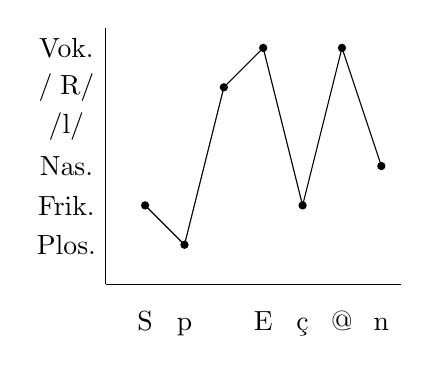
\begin{tikzpicture}[scale=0.5]
\draw[black] (-1,0) -- (6.5,0) ; % x axis
\draw[black] (-1,0) -- (-1,6.5); % y axis
\node at (-2,1) {Plos.};
\node at (-2,2) {Frik.};
\node at (-2,3) {Nas.};
\node at (-2,4) {\textipa{/l/}};
\node at (-2,5) {\textipa{/\;R/}};
\node at (-2,6) {Vok.};
\draw[black] (0,2) -- (1,1) -- (2,5) -- (3,6) -- (4,2) -- (5,6) -- (6,3);
\node at (0,-1) {\strut \textipa{S}};
\node at (1,-1) {\strut \textipa{p}};
\node at (2,-1) {\strut \textipa{\textscr}};
\node at (3,-1) {\strut \textipa{E}};
\node at (4,-1) {\strut \textipa{\c{c}}};
\node at (5,-1) {\strut \textipa{@}};
\node at (6,-1) {\strut \textipa{n}};
\fill (0,2) circle [radius=3pt];
\fill (1,1) circle [radius=3pt];
\fill (2,5) circle [radius=3pt];
\fill (3,6) circle [radius=3pt];
\fill (4,2) circle [radius=3pt];
\fill (5,6) circle [radius=3pt];
\fill (6,3) circle [radius=3pt];
\end{tikzpicture}}}
\end{figure}
\end{minipage}
\pause
\begin{minipage}{.05\textwidth}
\hfill
\end{minipage}
\begin{minipage}{.45\textwidth}
\begin{figure}
\centering
%\visible<4->
{\scalebox{.75}{
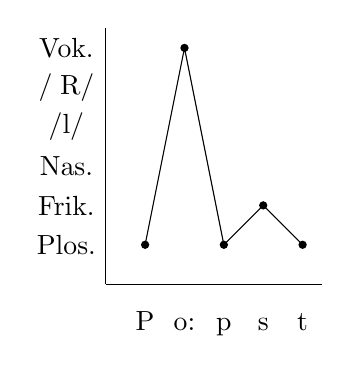
\begin{tikzpicture}[scale=0.5]
\draw[black] (-1,0) -- (4.5,0) ; % x axis
\draw[black] (-1,0) -- (-1,6.5); % y axis
\node at (-2,1) {Plos.};
\node at (-2,2) {Frik.};
\node at (-2,3) {Nas.};
\node at (-2,4) {\textipa{/l/}};
\node at (-2,5) {\textipa{/\;R/}};
\node at (-2,6) {Vok.};
\draw[black] (0,1) -- (1,6) -- (2,1) -- (3,2) -- (4,1);
\node at (0,-1) {\strut \textipa{P}};
\node at (1,-1) {\strut \textipa{o:}};
\node at (2,-1) {\strut \textipa{p}};
\node at (3,-1) {\strut \textipa{s}};
\node at (4,-1) {\strut \textipa{t}};
\fill (0,1) circle [radius=3pt];
\fill (1,6) circle [radius=3pt];
\fill (2,1) circle [radius=3pt];
\fill (3,2) circle [radius=3pt];
\fill (4,1) circle [radius=3pt];
\end{tikzpicture}}}
\end{figure}
\end{minipage}

\end{frame}
%%%%%%%%%%%%%%%%%%%%%%%%%%%%%%%%%

\begin{frame}
\frametitle{Übung -- Lösung}
%
\begin{minipage}{.3\textwidth}
\centering
\scalebox{.75}{\begin{forest} MyP edges, [,phantom
[$\sigma$
[O
[x, tier=word[\textipa{b}]]
[x, tier=word[\textipa{\textscr}]]
]
[R
[N	[x, tier=word[\textipa{a}]]
]
[K
[x[\textipa{n}]]
[x[\textipa{t}]]
]
]  
]
[$\sigma$
[O	[x, tier=word[\textipa{S}]]
]
[R	
[N	
[x[\textipa{U}]]
]
[K	
[x[\textipa{\t{ts}}]]
]
]
]]
\end{forest}}

\end{minipage}
\pause
%
\begin{minipage}{.02\textwidth}
\hfill
\end{minipage}
%
\begin{minipage}{.65\textwidth}
\centering
\scalebox{.75}{
\begin{forest}
MyP edges, [, phantom
[$ \sigma $
[O
[x, tier=word[\textipa{P}]]
]
[R
[N
[x, tier=word[\textipa{a}]]
]
[K
[x[\textipa{p}]]
]
]
]
[$ \sigma $
[O
[x, tier=word[\textipa{S}]]
[x, tier=word[\textipa{t}]]
]
[R
[N
[x[\textipa{a}]]
]
[K
[x[\textipa{n}]]
[x[\textipa{t}]]
[x[\textipa{s}]]
]
]
]
[$ \sigma $
[O
[x, tier=word[\textipa{h}]]
]
[R
[N
[x[\textipa{a}]]
]
[K
[x[\textipa{l}]]
]
]
]
[$ \sigma $
[O
[x, tier=word[t]]
]
[R	
[N
[x[\textipa{\textturna}]]
]
]
]]
\end{forest}}
\end{minipage}
\pause
\begin{minipage}{.3\textwidth}
\begin{figure}
\centering
\scalebox{.75}{
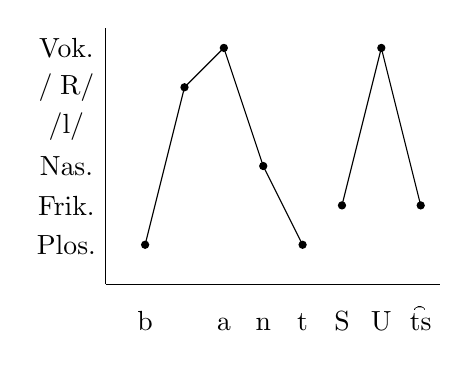
\begin{tikzpicture}[scale=0.5]
\draw[black] (-1,0) -- (7.5,0) ; % x axis
\draw[black] (-1,0) -- (-1,6.5); % y axis
\node at (-2,1) {Plos.};
\node at (-2,2) {Frik.};
\node at (-2,3) {Nas.};
\node at (-2,4) {\textipa{/l/}};
\node at (-2,5) {\textipa{/\;R/}};
\node at (-2,6) {Vok.};
\draw[black] (0,1) -- (1,5) -- (2,6) -- (3,3) -- (4,1);
\draw[black] (5,2) -- (6,6) -- (7,2);
\node at (0,-1) {\strut \textipa{b}};
\node at (1,-1) {\strut \textipa{\textscr}};
\node at (2,-1) {\strut \textipa{a}};
\node at (3,-1) {\strut \textipa{n}};
\node at (4,-1) {\strut \textipa{t}};
\node at (5,-1) {\strut \textipa{S}};
\node at (6,-1) {\strut \textipa{U}};
\node at (7,-1) {\strut \textipa{\t{ts}}};
\fill (0,1) circle [radius=3pt];
\fill (1,5) circle [radius=3pt];
\fill (2,6) circle [radius=3pt];
\fill (3,3) circle [radius=3pt];
\fill (4,1) circle [radius=3pt];
\fill (5,2) circle [radius=3pt];
\fill (6,6) circle [radius=3pt];
\fill (7,2) circle [radius=3pt];
\end{tikzpicture}}
\end{figure}
\end{minipage}
\pause
\begin{minipage}{.05\textwidth}
\hfill
\end{minipage}
\begin{minipage}{.6\textwidth}
\begin{figure}
\centering
\scalebox{.75}{
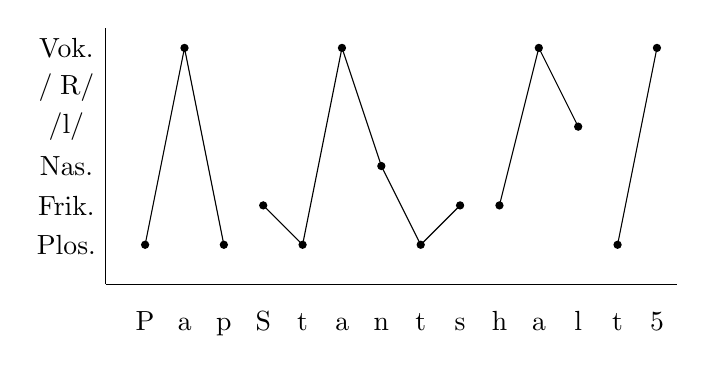
\begin{tikzpicture}[scale=0.5]
\draw[black] (-1,0) -- (13.5,0) ; % x axis
\draw[black] (-1,0) -- (-1,6.5); % y axis
\node at (-2,1) {Plos.};
\node at (-2,2) {Frik.};
\node at (-2,3) {Nas.};
\node at (-2,4) {\textipa{/l/}};
\node at (-2,5) {\textipa{/\;R/}};
\node at (-2,6) {Vok.};
\draw[black] (0,1)--(1,6)--(2,1);
\draw[black](3,2)--(4,1)--(5,6)--(6,3)--(7,1)--(8,2);
\draw[black](9,2)--(10,6)--(11,4);
\draw[black](12,1)--(13,6);
\fill (0,1) circle [radius=3pt];
\fill (1,6) circle [radius=3pt];
\fill (2,1) circle [radius=3pt];
\fill (3,2) circle [radius=3pt];
\fill (4,1) circle [radius=3pt];
\fill (5,6) circle [radius=3pt];
\fill (6,3) circle [radius=3pt];
\fill (7,1) circle [radius=3pt];
\fill (8,2) circle [radius=3pt];
\fill (9,2) circle [radius=3pt];
\fill (10,6) circle [radius=3pt];
\fill (11,4) circle [radius=3pt];
\fill (12,1) circle [radius=3pt];
\fill (13,6) circle [radius=3pt];
\node at (0,-1){\strut \textipa{P}};
\node at (1,-1){\strut \textipa{a}};
\node at (2,-1){\strut \textipa{p}};
\node at (3,-1){\strut \textipa{S}};
\node at (4,-1){\strut \textipa{t}};
\node at (5,-1){\strut \textipa{a}};
\node at (6,-1){\strut \textipa{n}};
\node at (7,-1){\strut \textipa{t}};
\node at (8,-1){\strut \textipa{s}};
\node at (9,-1){\strut \textipa{h}};
\node at (10,-1){\strut \textipa{a}};
\node at (11,-1){\strut \textipa{l}};
\node at (12,-1){\strut \textipa{t}};
\node at (13,-1){\strut \textipa{5}};
\end{tikzpicture}}
\end{figure}
\end{minipage}


\end{frame}

}

%%%%%%%%%%%%%%%%%%%%%%%%%%%%%%%%%%


%%%%%%%%%%%%%%%%%%%%%%%%%%%%%%%%%%
\subsection{Silbifizierung}

%% MyP: Contents
\iftoggle{sectoc}{
	\frame{
		%\begin{multicols}{2}
		\frametitle{~}
		\tableofcontents[currentsubsection, subsubsectionstyle=hide]
		%\end{multicols}
	}
}

%% StM: Contents
\iftoggle{gliederung}{
	
	\outline{
		\begin{itemize}
			
			\item Silbenmodelle
			%% CV-Modell
			%% Konstituentenmodell
			\item Silbengelenk
			\item \blaubf{Silbifizierung}
			\item Exkurs: Akzent
			\item Hausaufgabe
			
		\end{itemize}
	}
}
%%%%%%%%%%%%%%%%%%%%%%%%%%%%%%%%%%

\begin{frame}
\frametitle{Silbifizierung}

\begin{block}{Silbifizierung (auch Syllabierung)}
	Wörter in Silben einteilen
\end{block}

\begin{itemize}
	\item Wie würden Sie folgende Lautsequenzen silbifizieren?
	
	\ea ata, odo, eke
	\z
	
	\pause
	
	\item Ein einziger intervokalischer Konsonant wird immer als Silbenanlaut silbifiziert (universelles Prinzip: \textbf{Onset-Maximierung}).


\end{itemize}

\begin{block}{Onset-Maximierung}
Bilde zuerst den größtmöglichen Silbenanlaut;\\
dann bilde den Silbenauslaut \citep[218]{Hall00a}.
\end{block}

\end{frame}


%%%%%%%%%%%%%%%%%%%%%%%%%%%%%%%%%%
\begin{frame}
\frametitle{Onset-Maximierung}

\begin{block}{Onset-Maximierung}
Bilde zuerst den größtmöglichen Silbenanlaut;\\
dann bilde den Silbenauslaut \citep[218]{Hall00a}.
\end{block}


\begin{itemize}
\item Onset-Maximierung herleitbar aus:
\begin{enumerate}
\item Silbenanlautgesetz (CV häufiger als V), und
\item Silbenauslautgesetz (CVC$^{n} >$ CVC$^{n+1}$, wobei $n \geq 0$)
\end{enumerate}

\pause
\item Silbifizierung nicht über Morphemgrenzen hinweg! (grob: Morphem = kleinste bedeutungstragende Einheit)
\item Ausnahme: Suffixe mit vokalischem Onset:

\ea
kind\#isch: \textipa{[kIn.dIS]}

\ex
kind\#lich: \textipa{[kInt.lI\c{c}]}
\z

\item \# := Morphemgrenze

% Wenn man Morphmgrenzenbedingung weglassen würde, ergäbe sich Bra. ndschutz

% rek.nen vs. re.gnen

\end{itemize}

\end{frame}


%%%%%%%%%%%%%%%%%%%%%%%%%%%%%%%%%%
%\subsection{Übung}
%
%%% MyP: Contents
%\iftoggle{sectoc}{
%	\frame{
%		%\begin{multicols}{2}
%		\frametitle{~}
%		\tableofcontents[currentsubsection, subsubsectionstyle=hide]
%		%\end{multicols}
%	}
%}
%%%%%%%%%%%%%%%%%%%%%%%%%%%%%%%%%%
\begin{frame}
\frametitle{Übung}

\begin{itemize}
	\item Was bedeutet die Annahme des Sonoritätsprinzips und der Onset-Maximierung für die folgenden Beispielwörter?
	
	\eal\label{ex:fabrik}
	\ex Fabrik
	\ex Imker
	\ex neblig
	\ex Falter
	\ex regnen
	\zl
\end{itemize}

\end{frame}


%%%%%%%%%%%%%%%%%%%%%%%%%%%%%%%%
\iftoggle{ue-loesung}{
	%%%%%%%%%%%%%%%%%%%%%%%%%%%%%%%%%%
%% UE 1 - 03c Phonologie
%%%%%%%%%%%%%%%%%%%%%%%%%%%%%%%%%%


\begin{frame}
\frametitle{Übung -- Lösung}

\begin{itemize}
	\item Was bedeutet die Annahme des Sonoritätsprinzips und der Onset-Maximierung für die folgenden Beispielwörter:
	
	\begin{exe}
	\exr{ex:fabrik}
	\settowidth\jamwidth{XXXXXXXXXXXXXXXXXXXXXXXXXXXXXXXXXXXX}
	\begin{xlist}
		\ex Fabrik\loesung{1}{\textipa{[fa.b\textscr ik]} (auch: \textipa{[fa.b\;Ri:k]} oder \textipa{[fa.b\;RIk]})}
		\ex Imker\loesung{2}{\textipa{[PIm.k5]}}
		\ex neblig\loesung{3}{\textipa{[ne:.blI\c{c}]}}
		\ex Falter\loesung{4}{\textipa{[fal.t5]}}
		\ex regnen\loesung{5}{\textipa{[\textscr e:.gn@n]}}
		
	\loesung{6}{Koda: *Obstruent vor Sonorant}
	\loesung{7}{Onset: *Sonorant vor Obstruent}
	
	\end{xlist}
\end{exe}
	
	\alertred{Onset-Maximierung ist nicht strikt. Alternativ ginge auch \textipa{[ne:p.lI\c{c}]}, \textipa{[\textscr e:k.n@n]}.}
	
\end{itemize}

\end{frame}	

}

%%%%%%%%%%%%%%%%%%%%%%%%%%%%%%%
\begin{frame}{Übung}

\begin{itemize}
	\item Welche Prinzipien bzw. Regularitäten werden verletzt bei:


	\eal\label{ex:ebbe}
	\ex \textipa{[PE.b@]}
	\ex \textipa{[PEb.@]}
	\ex \textipa{[PEp.@]}
	\ex \textipa{[PEp.b@]}
	\zl
	
\end{itemize}

\end{frame}


%%%%%%%%%%%%%%%%%%%%%%%%%%%%%%%%
\iftoggle{ue-loesung}{
	%%%%%%%%%%%%%%%%%%%%%%%%%%%%%%%%%%
%% UE 2 - 03c Phonologie
%%%%%%%%%%%%%%%%%%%%%%%%%%%%%%%%%%

\begin{frame}
\frametitle{Übung -- Lösung}
	\begin{itemize}

	\item Welche Prinzipien bzw. Regularitäten werden verletzt bei:


	\eal
	\settowidth\jamwidth{XXXXXXXXXXXXXXXXXXXXXXXXXXXXXXXXXXXX}
	
		\ex \textipa{[PE.b@]}\jambox{\only<1->{\textcolor{red}{
			\ras Kurzvokal} Lösung \zb Silbengelenk \textipa{[PE\.b@]}
		}}
		\ex \textipa{[PEb.@]}\loesung{2}{\ras Auslautverhärtung}
		\ex \textipa{[PEp.@]}\loesung{3}{\ras Onset-Maximierung}
		\ex \textipa{[PEp.b@]}\loesung{4}{\ras keine Regelverletzung}
	\zl

	\end{itemize}

\end{frame}

}

%%%%%%%%%%%%%%%%%%%%%%%%%%%%%%%
\begin{frame}
\frametitle{Übung}

\begin{itemize}
	\item Silbifizieren Sie folgende Segmentsequenzen \textbf{in zwei Schritten}:
	\begin{itemize}
		\item Onset-Maximierungsprinzip
		\item Sonoritätsprinzip
	\end{itemize}
	
	\item Stellen Sie fest, ob alle Silben wohlgeformt sind.\\
	Falls nicht, benennen Sie die Verletzungen.
	
	\ea\label{ex:otling}
	\textipa{[o:tlIN5mSplag\textscr e:hOn]}
	\z
	
	% Otlingamsplagrehon
	
	\ea\label{ex:blumen}
	Blumentopferde
	\z
	
\end{itemize}

% blu.men.to.pfer.de

%\ea
%Urinstinkt
%\z	

\end{frame}


%%%%%%%%%%%%%%%%%%%%%%%%%%%%%%%%%%
\iftoggle{ue-loesung}{
	%%%%%%%%%%%%%%%%%%%%%%%%%%%%%%%%%%
%% UE 3 - 03c Phonologie
%%%%%%%%%%%%%%%%%%%%%%%%%%%%%%%%%%

\begin{frame}
\frametitle{Übung -- Lösung}

\begin{itemize}
\item Silbifizieren Sie folgende Segmentsequenzen \textbf{in zwei Schritten}:
\begin{itemize}
	\item Onsetmaximierungsprinzip
	\item Sonoritätsprinzip
\end{itemize}

\item Stellen Sie fest, ob alle Silben wohlgeformt sind.\\
Falls nicht, benennen Sie die Verletzungen.

\begin{exe}
	\exr{ex:otling}
	\textipa{[o:tlIN5mSplag\textscr e:hOn]}\\
	\alertred{zuerst Onset"=Maximierung: \textipa{o: . tlI . \ng {\textturna} . mSpla . g\textscr e: . hOn}\\
	dann Anwendung des Sonoritätsprinzips: \textipa{o: . tlI\. \ng \textturna mS . pla . g\textscr e: . hOn}}
\end{exe}

% Otlingamsplagrehon

\begin{exe}
	\exr{ex:blumen}
	Blumentopferde\\ \pause
	\alertred{zuerst Onset-Maximierung: \textipa{blu: . m@ . ntO . pfE . {\textscr}d@}\\
	dann Awendung des Sonoritätsprinzips: \textipa{blu: . m@n . tO . pfE{\textscr} . d@}}
\end{exe}

\end{itemize}

% blu.men.to.pfer.de

%\ea
%Urinstinkt
%\z	

\end{frame}


% ' Stahl , tische     Hauptbetonung auf Stahl, Nebenbetonung auf Tische


}

%%%%%%%%%%%%%%%%%%%%%%%%%%%%%%%%%%


%%%%%%%%%%%%%%%%%%%%%%%%%%%%%%%%%%
\subsection{Exkurs: Akzent}
%%%%%%%%%%%%%%%%%%%%%%%%%%%%%%%%%%

%% MyP: Contents
\iftoggle{sectoc}{
	\frame{
		%\begin{multicols}{2}
		\frametitle{~}
		\tableofcontents[currentsubsection, subsubsectionstyle=hide]
		%\end{multicols}
	}
}

%% StM: Contents
\iftoggle{gliederung}{
	
	\outline{
		\begin{itemize}
			
			\item Silbenmodelle
			%% CV-Modell
			%% Konstituentenmodell
			\item Silbengelenk
			\item Silbifizierung
			\item \blaubf{Exkurs: Akzent}
			\item Hausaufgabe
			
		\end{itemize}
	}
}
%%%%%%%%%%%%%%%%%%%%%%%%%%%%%%%%%%

\begin{frame}
\frametitle{Exkurs: Akzent}

\begin{itemize}
\item Silben können \textbf{betont} oder \textbf{unbetont} sein, d.\,h. sie können einen Akzent tragen oder nicht.
\item[]

\begin{block}{Akzent}
\textbf{Auditiver Eindruck der Prominenz eines Vokals} gegenüber einem anderen durch (relational, nicht absolut!):
\begin{itemize}
\item Lautstärke
\item Dauer
\item Höhere Tonlage
\item Ausgeprägtere Artikulationsbewegungen
\end{itemize}
\end{block}	 

\item[]
\item Man unterscheidet zwischen \textbf{Wort-} und \textbf{Satzakzent} (engl. \emph{stress} und \emph{accent}).

\end{itemize}

\end{frame}



%%%%%%%%%%%%%%%%%%%%%%%%%%%%%%%%%%%
%%%%%%%%%%%%%%%%%%%%%%%%%%%%%%%%%%
%\subsubsection{Exkurs: Wortakzent}
%\frame{
%\begin{multicols}{2}
%\frametitle{~}
%	\tableofcontents[currentsection]
%\end{multicols}
%}
%%%%%%%%%%%%%%%%%%%%%%%%%%%%%%%%%%

\begin{frame}
\frametitle{Exkurs: Wortakzent}

\begin{itemize}
\item Was scheint die häufigste Betonung im Deutschen zu sein?

\ea
Mutter, Männer, Autos, Hühner, Lehrer, Kinder, alle, \ldots
\z

\pause
\textbf{betont-unbetont (Trochäus)}

\item Ausnahmen (die je nach Theorie verschieden erklärt werden):

\end{itemize}

\begin{minipage}{.4\textwidth}

\eal 
\ex \textipa{['f\textscr aU]}
\ex \textipa{[mu.'zi:k]}
\ex \textipa{['le:.b@n.d@]}
\ex \textipa{[pa.pa.'g\t{aɪ}]}
\ex \textipa{[f\t{ɛɐ}.'Pa\textscr .b\t{aɪ}.t@n]}
\zl

\end{minipage}
\begin{minipage}{.5\textwidth}

%	\iftoggle{loesung}{
\begin{itemize}
\item[] \alertred{\ras nur eine Silbe }
\item[] \alertred{\ras Fremdwort}
\item[] \alertred{\ras flektierte Elemente \ab{-de}}
\item[] \alertred{\ras Fremdwort}
\item[] \alertred{\ras Derivation \ab{ver-}}
\end{itemize}
%}

\end{minipage}

\end{frame}



%%%%%%%%%%%%%%%%%%%%%%%%%%%%%%%%%%%
%%%%%%%%%%%%%%%%%%%%%%%%%%%%%%%%%%
%\subsubsection{Exkurs: Satzakzent}
%\frame{
%\begin{multicols}{2}
%\frametitle{~}
%	\tableofcontents[currentsection]
%\end{multicols}
%}
%%%%%%%%%%%%%%%%%%%%%%%%%%%%%%%%%%

\begin{frame}
\frametitle{Exkurs: Satzakzent}

\begin{itemize}
\item In einem Satz können betonte Silben \textbf{noch weiter hervorgehoben} werden (dabei meist durch die Tonhöhe):

\eal 
\ex Géstern hat BÁyern gewónnen.
\ex GÉStern hat Báyern gewónnen.
\ex Géstern hat Báyern geWÓNnen.
\zl
\item Die prominenteste Silbe im Satz wird meist mit \textbf{Großbuchstaben} dargestellt, sie trägt den Satzakzent.

\item Durch diese Akzentuierung wird das gesamte Wort
hervorgehoben.\\
\ras \textbf{Fokus des Satzes} (\gqq{Informationsstruktur})

\end{itemize}

\end{frame}



%%%%%%%%%%%%%%%%%%%%%%%%%%%%%%%%%%%
%%%%%%%%%%%%%%%%%%%%%%%%%%%%%%%%%%
%\subsubsection{Exkurs: Intonation}
%\frame{
%\begin{multicols}{2}
%\frametitle{~}
%	\tableofcontents[currentsection]
%\end{multicols}
%}
%%%%%%%%%%%%%%%%%%%%%%%%%%%%%%%%%%

\begin{frame}
\frametitle{Exkurs: Intonation}

\begin{block}{Intonation}
Tonhöhenverlauf (\gqq{Melodie}) einer Äußerung
\end{block}

\begin{itemize}
\item \textbf{Satztypen} können mittels Intonation unterschieden werden.

\item Sprechen Sie die folgenden Äußerungen mit fallender und steigender Intonation.
\eal 
\ex Heute gewinnen die Bayern.
\ex Schon Schluss.
\zl
\pause
\textbf{Aussage-} \vs \textbf{Interrogativsatz}	

\end{itemize}

\end{frame}



%%%%%%%%%%%%%%%%%%%%%%%%%%%%%%%%%%

\begin{frame}
\frametitle{Disambiguierung}

Ambige ($\approx$ mehrdeutige) Sätze können mittels Intonation \gs{durch die sog. Hutkontur} \textbf{disambiguiert} werden: 

\begin{exe}
\ex  \label{exe:nicht}Alle Studenten haben die Klausur nicht bestanden.

	\begin{xlist}
	\ex Es ist nicht der Fall, dass alle Studenten die Klausur bestanden haben. \hfill $\lsem \neg \forall \rsem$
	\ex Für alle Studenten gilt, dass sie die Klausur nicht bestanden haben. \hfill $\lsem \forall \neg \rsem$
	\end{xlist}

\pause 

\ex /ALle Studenten haben die Klausur  NICHT\textbackslash\ bestanden.
\exr{exe:nicht}
	\begin{xlist}
	\ex Es ist nicht der Fall, dass alle Studenten die Klausur bestanden haben. \hfill $\lsem \neg \forall \rsem$
	\end{xlist}
\end{exe}


\end{frame}


%%%%%%%%%%%%%%%%%%%%%%%%%%%%%%%%%%
\subsection{Hausaufgabe}
%%%%%%%%%%%%%%%%%%%%%%%%%%%%%%%%%%

%%% MyP: Contents
%\iftoggle{sectoc}{
%	\frame{
%		%\begin{multicols}{2}
%		\frametitle{~}
%		\tableofcontents[currentsubsection, subsubsectionstyle=hide]
%		%\end{multicols}
%	}
%}

%%% StM: Contents
%\iftoggle{gliederung}{
%	
%	\outline{
%		\begin{itemize}
%			
%			\item Silbenmodelle
%			%% CV-Modell
%			%% Konstituentenmodell
%			\item Silbengelenk
%			\item Silbifizierung
%			\item Exkurs: Akzent
%			\item \blaubf{Hausaufgabe}
%			
%		\end{itemize}
%	}
%}


%%%%%%%%%%%%%%%%%%%%%%%%%%%%%%%%%%
\begin{frame}%[allowframebreaks]
\frametitle{Hausaufgabe}
\begin{itemize}

\item[1.] Geben Sie eine \textbf{phonetische Transkription} der folgenden Wörter nach der \gqq{Standardaussprache} an, zeichnen Sie dabei die \textbf{Silbenstruktur} nach dem \textbf{Konstituentenmodell} und mit der \textbf{Skelettschicht} und geben Sie die \textbf{Sonoritätsprofile} an.

\eal\label{ex:03cHA1}
\ex Stimmenfang \label{ex:03cHA1a}
\ex Mittagessen\label{ex:03cHA1b}
\ex Bierdeckel\label{ex:03cHA1c}
\zl
\end{itemize}

\begin{block}{Sonoritätshierarchie (Zur Erinnerung)}
Vokal $>$ \textipa{/\textscr /} $>$ \textipa{/l/} $>$ Nasal $>$ Frikativ $>$ Plosiv \\
$x > y$ := $x$ ist sonorer als $y$
\end{block}

\end{frame}

%%%%%%%%%%%%%%%%%%%%%%%%%%%%%%%%%%%%%%%%%%%%%%%%%%%%%

\begin{frame}
\begin{itemize}
\item[2.] Silbifizieren Sie folgende Segmentsequenzen \textbf{in zwei Schritten}:
\begin{itemize}
\item Onset-Maximierungsprinzip
\item Sonoritätsprinzip
\end{itemize}

Stellen Sie fest, ob alle Silben wohlgeformt sind. Falls nicht, benennen Sie die Verletzungen.
\ea\label{ex:03cHA2}
Urinstinkt
\z	
\item[3.] Geben Sie die standarddeutsche \textbf{phonetische Transkription} des Wortes \ab{Stahltische} inklusive der \textbf{Silbenstruktur} (mit X-Skelettschicht) an.\\Ermitteln Sie die \textbf{Kriterien}, die bei der Silbifizierung wirken.

\item[4.] Geben Sie die Gründe an, warum die folgenden Wörter aus phonetisch"=phonologischen Gründen im Deutschen nicht möglich sind:

\eal\label{ex:03cHA3}
\ex[*]{\textipa{['Napl.O:t]}}
\ex[*]{\textipa{[a\;R.'tUng]}}
\zl

\end{itemize}

\end{frame}

%%%%%%%%%%%%%%%%%%%%%%%%%%%%%%%%%%%
\iftoggle{ha-loesung}{
	%%%%%%%%%%%%%%%%%%%%%%%%%%%%%%%%%%
%% HA 1 - 03c Phonologie
%%%%%%%%%%%%%%%%%%%%%%%%%%%%%%%%%%

\begin{frame}%[allowframebreaks]
\frametitle{Hausaufgabe -- Lösung}
\begin{itemize}

\item[1.] Geben Sie eine \textbf{phonetische Transkription} der folgenden Wörter nach der \gqq{Standardaussprache} an, zeichnen Sie dabei die \textbf{Silbestruktur} nach dem \textbf{Konstituentenmodell} und mit der \textbf{Skelettschicht} und geben Sie die \textbf{Sonoritätsprofile} an.

\begin{exe}
\exi{(\ref{ex:03cHA1})}
\begin{xlist}
\ex Stimmenfang
\ex Mittagessen
\ex Bierdeckel
\end{xlist}
\end{exe}

\begin{block}{Sonoritätshierarchie (Zur Erinnerung)}
Vokal $>$ \textipa{/\textscr /} $>$ \textipa{/l/} $>$ Nasal $>$ Frikativ $>$ Plosiv \\
$x > y :=$ $x$ ist sonorer als $y$
\end{block}

\end{itemize}
\end{frame}
%%%%%%%%%%%%%%%%%%%%%%%%%%%%%%%%%%

\begin{frame}{Hausaufgabe -- Lösung}

Zu (\ref{ex:03cHA1a}):

\begin{columns}	
	
\column[b]{.5\textwidth}

\begin{figure}
%	\footnotesize
	\centering
	\begin{forest} MyP edges, [, phantom
		[$\sigma$
		[O [x, tier=word [\textipa{S}]] [x, tier=word [\textipa{t}]]]
		[R [N [x, tier=word [\textipa{I}]]] [K [x, name=x [\textipa{m}]]]]
		]
		[$\sigma$
		[O, name=onset]
		[R [N [x [\textipa{@}]]] [K [x [\textipa{n}]]]]
		]
		[$\sigma$
		[O [x, tier=word [\textipa{f}]]]
		[R [N [x [\textipa{a}]]] [K [x [\textipa{N}]]]]
		]
		]				
		{
		\draw[black] (x.north)--(onset.south);
		}
	\end{forest}
\end{figure}

\pause

\column[b]{.5\textwidth}

\begin{figure}
%	\footnotesize
	\centering	
	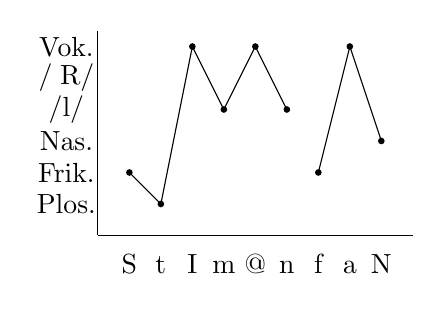
\begin{tikzpicture}[scale=0.4]
		\draw[black] (-1,0) -- (9,0) ; % x axis
		\draw[black] (-1,0) -- (-1,6.5); % y axis
		\node at (-2,1) {Plos.};
		\node at (-2,2) {Frik.};
		\node at (-2,3) {Nas.};
		\node at (-2,4) {\textipa{/l/}};
		\node at (-2,5) {\textipa{/\;R/}};
		\node at (-2,6) {Vok.};
		\draw[black] (0,2) -- (1,1) -- (2,6) -- (3,4) -- (4,6) -- (5,4);
		\draw[black] (6,2) -- (7,6) -- (8,3);
		\node at (0,-1) {\strut \textipa{S}};
		\node at (1,-1) {\strut \textipa{t}};
		\node at (2,-1) {\strut \textipa{I}};
		\node at (3,-1) {\strut \textipa{m}};
		\node at (4,-1) {\strut \textipa{@}};
		\node at (5,-1) {\strut \textipa{n}};
		\node at (6,-1) {\strut \textipa{f}};
		\node at (7,-1) {\strut \textipa{a}};
		\node at (8,-1) {\strut \textipa{N}};
		\fill (0,2) circle [radius=3pt];
		\fill (1,1) circle [radius=3pt];
		\fill (2,6) circle [radius=3pt];
		\fill (3,4) circle [radius=3pt];
		\fill (4,6) circle [radius=3pt];
		\fill (5,4) circle [radius=3pt];
		\fill (6,2) circle [radius=3pt];
		\fill (7,6) circle [radius=3pt];
		\fill (8,3) circle [radius=3pt];
	\end{tikzpicture}
\end{figure}

\end{columns}

\end{frame}


%%%%%%%%%%%%%%%%%%%%%%%%%%%%%%%%%%%%%%%%%%%%%%%
\begin{frame}{Hausaufgabe -- Lösung}


Zu (\ref{ex:03cHA1b})

\begin{columns}
	\column[b]{.5\textwidth}
	
\begin{figure}
\footnotesize
\centering
	\begin{forest} MyP edges, [, phantom
		[$\sigma$
		[O [x, tier=word [\textipa{m}]]] 
		[R [N [x, tier=word [\textipa{I}]]] [K [x, name=x1 [\textipa{t}]]]]
		]
		[$\sigma$
		[O, name=onset1]
		[R [N [x [\textipa{a:}, name=a]]
		[x, name=ax]] [K [x [\textipa{k}]]]]
		]
		[$\sigma$
		[O [x, tier=word [\textipa{P}]]]
		[R [N [x [\textipa{E}]]] [K [x, name=x2 [\textipa{s}]]]]
		]
		[$\sigma$
		[O, name=onset2]
		[R [N [x [\textipa{\textsyllabic{n}}]]]
		]
		]]
		{
		\draw[black] (x1.north)--(onset1.south);
		\draw[black] (x2.north)--(onset2.south);
		\draw[black] (a.north)--(ax.south);
		}
	\end{forest}
\end{figure}

\pause
\column[b]{.5\textwidth}

\begin{figure}
	\footnotesize
	\centering
	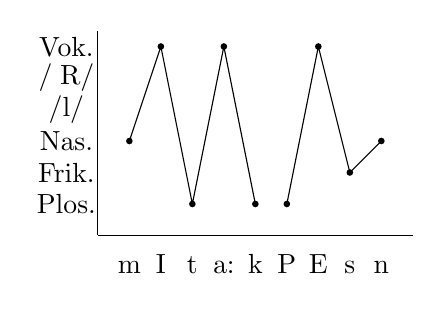
\begin{tikzpicture}[scale=0.4]
		\draw[black] (-1,0) -- (9,0) ; % x axis
		\draw[black] (-1,0) -- (-1,6.5); % y axis
		\node at (-2,1) {Plos.};
		\node at (-2,2) {Frik.};
		\node at (-2,3) {Nas.};
		\node at (-2,4) {\textipa{/l/}};
		\node at (-2,5) {\textipa{/\;R/}};
		\node at (-2,6) {Vok.};
		\draw[black] (0,3) -- (1,6) -- (2,1) -- (3,6) -- (4,1);
		\draw[black] (5,1) -- (6,6) -- (7,2) -- (8,3);
		\node at (0,-1) {\strut \textipa{m}};
		\node at (1,-1) {\strut \textipa{I}};
		\node at (2,-1) {\strut \textipa{t}};
		\node at (3,-1) {\strut \textipa{a:}};
		\node at (4,-1) {\strut \textipa{k}};
		\node at (5,-1) {\strut \textipa{P}};
		\node at (6,-1) {\strut \textipa{E}};
		\node at (7,-1) {\strut \textipa{s}};
		\node at (8,-1) {\strut \textipa{\textsyllabic{n}}};
		\fill (0,3) circle [radius=3pt];
		\fill (1,6) circle [radius=3pt];
		\fill (2,1) circle [radius=3pt];
		\fill (3,6) circle [radius=3pt];
		\fill (4,1) circle [radius=3pt];
		\fill (5,1) circle [radius=3pt];
		\fill (6,6) circle [radius=3pt];
		\fill (7,2) circle [radius=3pt];
		\fill (8,3) circle [radius=3pt];
	\end{tikzpicture}
\end{figure}

\end{columns}

\end{frame}


%%%%%%%%%%%%%%%%%%%%%%%%%%%%%%%%%%%%%%%%%%%%
\begin{frame}{Hausaufgabe -- Lösung}

Zu (\ref{ex:03cHA1b})  (alternative Lösung):

\begin{columns}
	\column[b]{.5\textwidth}
	
	
\begin{figure}
\footnotesize
\centering

	\begin{forest} MyP edges, [, phantom
		[$\sigma$
		[O [x, tier=word [\textipa{m}]]] 
		[R [N [x, tier=word [\textipa{I}]]] [K [x, name=x1 [\textipa{t}]]]]
		]
		[$\sigma$
		[O, name=onset1]
		[R [N [x [\textipa{a:}, name=a]]
		[x, name=ax]] [K [x [\textipa{k}]]]]
		]
		[$\sigma$
		[O [x, tier=word [\textipa{P}]]]
		[R [N [x [\textipa{E}]]] [K [x, name=x2 [\textipa{s}]]]]
		]
		[$\sigma$
		[O, name=onset2]
		[R [N [x [\textipa{@}]]] [K [x [\textipa{n}]]]]
		]
		]
		{
		\draw[black] (x1.north)--(onset1.south);
		\draw[black] (x2.north)--(onset2.south);
		\draw[black] (a.north)--(ax.south);
		}
	\end{forest}

\end{figure}

\pause

\column[b]{.5\textwidth}

\begin{figure}
\footnotesize
\centering
	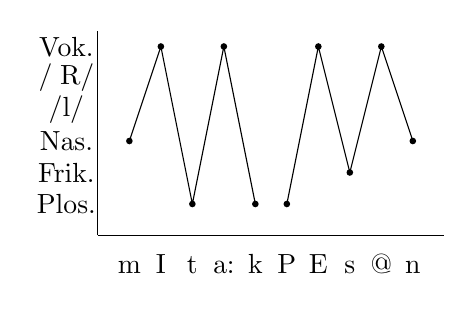
\begin{tikzpicture}[scale=0.4]
		\draw[black] (-1,0) -- (10,0) ; % x axis
		\draw[black] (-1,0) -- (-1,6.5); % y axis
		\node at (-2,1) {Plos.};
		\node at (-2,2) {Frik.};
		\node at (-2,3) {Nas.};
		\node at (-2,4) {\textipa{/l/}};
		\node at (-2,5) {\textipa{/\;R/}};
		\node at (-2,6) {Vok.};
		\draw[black] (0,3) -- (1,6) -- (2,1) -- (3,6) -- (4,1);
		\draw[black] (5,1) -- (6,6) -- (7,2) -- (8,6) -- (9,3);
		\node at (0,-1) {\strut \textipa{m}};
		\node at (1,-1) {\strut \textipa{I}};
		\node at (2,-1) {\strut \textipa{t}};
		\node at (3,-1) {\strut \textipa{a:}};
		\node at (4,-1) {\strut \textipa{k}};
		\node at (5,-1) {\strut \textipa{P}};
		\node at (6,-1) {\strut \textipa{E}};
		\node at (7,-1) {\strut \textipa{s}};
		\node at (8,-1) {\strut \textipa{@}};
		\node at (9,-1) {\strut \textipa{n}};
		\fill (0,3) circle [radius=3pt];
		\fill (1,6) circle [radius=3pt];
		\fill (2,1) circle [radius=3pt];
		\fill (3,6) circle [radius=3pt];
		\fill (4,1) circle [radius=3pt];
		\fill (5,1) circle [radius=3pt];
		\fill (6,6) circle [radius=3pt];
		\fill (7,2) circle [radius=3pt];
		\fill (8,6) circle [radius=3pt];
		\fill (9,3) circle [radius=3pt];
	\end{tikzpicture}
\end{figure}

\end{columns}

\end{frame}


%%%%%%%%%%%%%%%%%%%%%%%%%%%%%%%%%%%%%%%%%%%%%%%
\begin{frame}{Hausaufgabe -- Lösung}

Zu (\ref{ex:03cHA1c}):

\begin{columns}
	\column[b]{.5\textwidth}
	
\begin{figure}
\centering
	\begin{forest} MyP edges, [, phantom
		[$\sigma$
		[O [x,tier=word [\textipa{b}]]]
		[R [N [x, tier=word [\textipa{i:}, name=i]] [x,name=x1]] [K [x [\textipa{5}]]]]
		]
		[$\sigma$
		[O [x, tier=word [\textipa{d}]]]
		[R [N [x [\textipa{E}]]] [K [x, name=x [\textipa{k}]]]]
		]
		[$\sigma$
		[O, name=onset]
		[R [N [x, tier=word [\textipa{@}]]] [K [x [\textipa{l}]]]]
		]
		]
		{
		\draw[black] (x1.south)--(i.north);
		\draw[black] (x.north)--(onset.south);
		}
	\end{forest}
\end{figure}

\pause

\column[b]{.5\textwidth}

\begin{figure}
\centering
	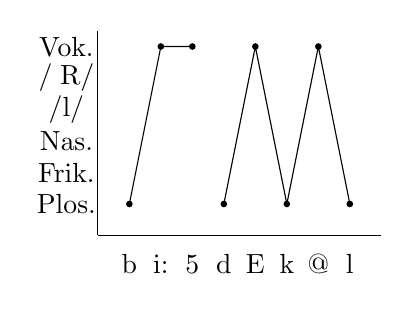
\begin{tikzpicture}[scale=0.4]
		\draw[black] (-1,0) -- (8,0) ; % x axis
		\draw[black] (-1,0) -- (-1,6.5); % y axis
		\node at (-2,1) {Plos.};
		\node at (-2,2) {Frik.};
		\node at (-2,3) {Nas.};
		\node at (-2,4) {\textipa{/l/}};
		\node at (-2,5) {\textipa{/\;R/}};
		\node at (-2,6) {Vok.};
		\draw[black] (0,1) -- (1,6) -- (2,6);
		\draw[black] (3,1) -- (4,6) -- (5,1) -- (6,6) -- (7,1);
		\node at (0,-1) {\strut \textipa{b}};
		\node at (1,-1) {\strut \textipa{i:}};
		\node at (2,-1) {\strut \textipa{5}};
		\node at (3,-1) {\strut \textipa{d}};
		\node at (4,-1) {\strut \textipa{E}};
		\node at (5,-1) {\strut \textipa{k}};
		\node at (6,-1) {\strut \textipa{@}};
		\node at (7,-1) {\strut \textipa{l}};
		\fill (0,1) circle [radius=3pt];
		\fill (1,6) circle [radius=3pt];
		\fill (2,6) circle [radius=3pt];
		\fill (3,1) circle [radius=3pt];
		\fill (4,6) circle [radius=3pt];
		\fill (5,1) circle [radius=3pt];
		\fill (6,6) circle [radius=3pt];
		\fill (7,1) circle [radius=3pt];
	\end{tikzpicture}
\end{figure}

\end{columns}

\end{frame}


%%%%%%%%%%%%%%%%%%%%%%%%%%%%%%%%%%%%%%%%%%%%%%%%%%%
\begin{frame}{Hausaufgabe -- Lösung}
\begin{itemize}
\item[2.] Silbifizieren Sie folgende Segmentsequenzen \textbf{in zwei Schritten}:
\begin{itemize}
\item Onsetmaximierungsprinzip
\item Sonoritätsprinzip
\end{itemize}

Stellen Sie fest, ob alle Silben wohlgeformt sind.\\
Falls nicht, benennen Sie die Verletzungen.

\begin{exe}
\exr{ex:03cHA2} Urinstinkt
\pause
\begin{xlist}
	\ex \alertred{\textipa{[Pu.\;RI.nStInkt]} (Onsetmaximierung)} \pause
	\ex  \alertred{\textipa{[Pu.\;RIn.(\,S\,)tInkt]} (Sonoritätsprinzip, \textipa{S} ist extrasilbisch)} \pause
	\ex  \alertred{\textipa{[Pu5.PIn.stinkt]} (Silbifizierung)}
\end{xlist}
\end{exe}
\pause

\item (\ref{ex:03cHA2}a) und (\ref{ex:03cHA2}b) sind einfach nach der Lautfolge silbifiziert.\\
Silbifizierung erfolgt jedoch auf der Ebene des phonologischen Wortes.\\
Daher werden die phonologischen Wörter \ab{ur-} und \ab{Instinkt} einzeln silbifiziert.
\end{itemize}
\end{frame}

%%%%%%%%%%%%%%%%%%%%%%%%%%%%%%%%%%%%%%%%%%%%%%%%

\begin{frame}{Hausaufgabe -- Lösung}
\begin{itemize}	
\item[3.] Geben Sie die standarddeutsche \textbf{phonetische Transkription} des Wortes \ab{Stahltische} inklusive der \textbf{Silbenstruktur} (mit X-Skelettschicht) an. Ermitteln Sie die \textbf{Kriterien}, die bei der Silbifizierung wirken.
\end{itemize}

\pause

\begin{minipage}{.5\textwidth}
\begin{figure}
\scalebox{.8}{\begin{forest}
MyP edges [, phantom
[$\sigma$
[O 
[x, tier=word[\textipa{S}]]
[x, tier=word[\textipa{t}]]
]
[R
[N
[x, tier=word[\textipa{a:}, name=a]]
[x, name=x]
]
[K[x[\textipa{l}]]]
]
]
[$\sigma$
[O [x, tier=word[\textipa{t}]]]
[R
[N
[x[\textipa{I}]]
]
[K
[x,name=S[\textipa{S}] ]
]
]
]
[$\sigma$
[O, name=o]
[R
[N
[x[\textipa{@}]]
]
]
]
]
\draw[black](o.south)--(S.north);
\draw[black](a.north)--(x.south);
\end{forest}}
\end{figure}
\end{minipage}
\begin{minipage}{.45\textwidth}
	
\pause	
	
\begin{itemize}
\item Onset-Maximierung \pause
\item Sonoritätshierarchie im Onset: *Sonorant vor Obstruent (*[\textipa{lt}]) \pause
\item Silbengelenk nach ungespanntem, betontem Vokal
\end{itemize}
\end{minipage}

\end{frame}

%%%%%%%%%%%%%%%%%%%%%%%%%%%%%%%%%%%%%

\begin{frame}{Hausaufgabe -- Lösung}
\begin{itemize}

\item[4.] Geben Sie die Gründe an, warum die folgenden Wörter aus phonetisch/""phonologischen Gründen im Deutschen nicht möglich sind:

\begin{exe}
	\exr{ex:03cHA3}
	\settowidth\jamwidth{XXXXXXXXXXXXXXXXXXXXXXXXXXXXXXXXXXX}
	\begin{xlist}
		\ex[*]{ \textipa{['Napl.O:t]}
			\loesung{2}{Onset-Maximierung \textipa{[pl]}, \textipa{[N]} steht am Wortanfang,} 
			\loesung{2}{\textipa{[O]} ist ungespannt und lang} }
		\ex[*]{ \textipa{[a\;R.'tUng]}
			\loesung{3}{Auslautverhärtung, regressive velare nasale Assimilation,}\loesung{3}{Knacklaut} }
	\end{xlist}

\end{exe}

\end{itemize}

\end{frame}

}

%%%%%%%%%%%%%%%%%%%%%%%%%%%%%%%%%%



%% -*- coding:utf-8 -*-

%%%%%%%%%%%%%%%%%%%%%%%%%%%%%%%%%%%%%%%%%%%%%%%%%%%%%%%%%


\def\insertsectionhead{\refname}
\def\insertsubsectionhead{}

\huberlinjustbarfootline


\ifpdf
\else
\ifxetex
\else
\let\url=\burl
\fi
\fi
\begin{multicols}{2}
{\tiny
%\beamertemplatearticlebibitems

\bibliography{gkbib,bib-abbr,biblio}
\bibliographystyle{unified}
}
\end{multicols}





%% \section{Literatur}
%% \begin{frame}[allowframebreaks]
%% \frametitle{Literatur}
%% 	\footnotesize

%% \bibliographystyle{unified}

%% 	%German
%% %	\bibliographystyle{deChicagoMyP}

%% %	%English
%% %	\bibliographystyle{chicago} 

%% 	\bibliography{gkbib,bib-abbr,biblio}
	
%% \end{frame}


\end{document}
